% ******************************* PhD Thesis Template **************************
% Please have a look at the README.md file for info on how to use the template

\documentclass[b5paper,11pt,times,custombib,print,index]{classes/PhDThesisPSnPDF}

% ******************************************************************************
% ******************************* Class Options ********************************
% *********************** See README for more details **************************
% ******************************************************************************

% `a4paper'(The University of Cambridge PhD thesis guidelines recommends a page
% size a4 - default option) or `a5paper': A5 Paper size is also allowed as per
% the Cambridge University Engineering Deparment guidelines for PhD thesis
%
% `11pt' or `12pt'(default): Font Size 10pt is NOT recommended by the University
% guidelines
%
% `oneside' or `twoside'(default): Printing double side (twoside) or single
% side.
%
% `print': Use `print' for print version with appropriate margins and page
% layout. Leaving the options field blank will activate Online version.
%
% `index': For index at the end of the thesis
%
% `draftclassic': For draft mode without loading any images (same as draft in book)
%
% `draft': Special draft mode with line numbers, images, and water mark with
% timestamp and custom text. Position of the text can also be modified.
%
% `abstract': To generate only the title page and abstract page with
% dissertation title and name, to submit to the Student Registry
%
% `chapter`: This option enables only the specified chapter and it's references
%  Useful for review and corrections.
%
% ************************* Custom Page Margins ********************************
%
% `custommargin`: Use `custommargin' in options to activate custom page margins,
% which can be defined in the preamble.tex. Custom margin will override
% print/online margin setup.
%
% *********************** Choosing the Fonts in Class Options ******************
%
% `times' : Times font with math support. (The Cambridge University guidelines
% recommend using times)
%
% `fourier': Utopia Font with Fourier Math font (Font has to be installed)
%            It's a free font.
%
% `customfont': Use `customfont' option in the document class and load the
% package in the preamble.tex
%
% default or leave empty: `Latin Modern' font will be loaded.
%
% ********************** Choosing the Bibliography style ***********************
%
% `authoryear': For author-year citation eg., Krishna (2013)
%
% `numbered': (Default Option) For numbered and sorted citation e.g., [1,5,2]
%
% `custombib': Define your own bibliography style in the `preamble.tex' file.
%              `\RequirePackage[square, sort, numbers, authoryear]{natbib}'.
%              This can be also used to load biblatex instead of natbib
%              (See Preamble)
%
% **************************** Choosing the Page Style *************************
%
% `default (leave empty)': For Page Numbers in Header (Left Even, Right Odd) and
% Chapter Name in Header (Right Even) and Section Name (Left Odd). Blank Footer.
%
% `PageStyleI': Chapter Name next & Page Number on Even Side (Left Even).
% Section Name & Page Number in Header on Odd Side (Right Odd). Footer is empty.
%
% `PageStyleII': Chapter Name on Even Side (Left Even) in Header. Section Number
% and Section Name in Header on Odd Side (Right Odd). Page numbering in footer

% Uncomment to change page style
%\pagestyle{PageStyleII}

% ********************************** Preamble **********************************
% Preamble: Contains packages and user-defined commands and settings
% ******************************************************************************
% ****************************** Custom Margin *********************************

% Add `custommargin' in the document class options to use this section
% Set {innerside margin / outerside margin / topmargin / bottom margin}  and
% other page dimensions
\ifsetCustomMargin
  \RequirePackage[left=37mm,right=30mm,top=35mm,bottom=30mm]{geometry}
  \setFancyHdr % To apply fancy header after geometry package is loaded
\fi

% Add spaces between paragraphs
%\setlength{\parskip}{0.5em}
% Ragged bottom avoids extra whitespaces between paragraphs
\raggedbottom
% To remove the excess top spacing for enumeration, list and description
%\usepackage{enumitem}
%\setlist[enumerate,itemize,description]{topsep=0em}

% *****************************************************************************
% ******************* Fonts (like different typewriter fonts etc.)*************

% Add `customfont' in the document class option to use this section

\ifsetCustomFont
  % Set your custom font here and use `customfont' in options. Leave empty to
  % load computer modern font (default LaTeX font).
  %\RequirePackage{helvet}

  % For use with XeLaTeX
  %  \setmainfont[
  %    Path              = ./libertine/opentype/,
  %    Extension         = .otf,
  %    UprightFont = LinLibertine_R,
  %    BoldFont = LinLibertine_RZ, % Linux Libertine O Regular Semibold
  %    ItalicFont = LinLibertine_RI,
  %    BoldItalicFont = LinLibertine_RZI, % Linux Libertine O Regular Semibold Italic
  %  ]
  %  {libertine}
  %  % load font from system font
  %  \newfontfamily\libertinesystemfont{Linux Libertine O}
\fi

% *****************************************************************************
% **************************** Custom Packages ********************************

% ************************* Algorithms and Pseudocode **************************

%\usepackage{algpseudocode}


% ********************Captions and Hyperreferencing / URL **********************

% Captions: This makes captions of figures use a boldfaced small font.
%\RequirePackage[small,bf]{caption}

\RequirePackage[labelsep=space,tableposition=top]{caption}
\renewcommand{\figurename}{Fig.} %to support older versions of captions.sty


% *************************** Graphics and figures *****************************

%\usepackage{rotating}
%\usepackage{wrapfig}

% Uncomment the following two lines to force Latex to place the figure.
% Use [H] when including graphics. Note 'H' instead of 'h'
%\usepackage{float}
%\restylefloat{figure}

% Subcaption package is also available in the sty folder you can use that by
% uncommenting the following line
% This is for people stuck with older versions of texlive
%\usepackage{sty/caption/subcaption}
\usepackage{subcaption}

% ********************************** Tables ************************************
\usepackage{booktabs} % For professional looking tables
\usepackage{multirow}

%\usepackage{multicol}
%\usepackage{longtable}
%\usepackage{tabularx}


% *********************************** SI Units *********************************
\usepackage{siunitx} % use this package module for SI units


% ******************************* Line Spacing *********************************

% Choose linespacing as appropriate. Default is one-half line spacing as per the
% University guidelines

% \doublespacing
% \onehalfspacing
% \singlespacing


% ************************ Formatting / Footnote *******************************

% Don't break enumeration (etc.) across pages in an ugly manner (default 10000)
%\clubpenalty=500
%\widowpenalty=500

%\usepackage[perpage]{footmisc} %Range of footnote options


% *****************************************************************************
% *************************** Bibliography  and References ********************

%\usepackage{cleveref} %Referencing without need to explicitly state fig /table

% Add `custombib' in the document class option to use this section
\ifuseCustomBib
   \RequirePackage[square, sort, numbers]{natbib} % CustomBib

% If you would like to use biblatex for your reference management, as opposed to the default `natbibpackage` pass the option `custombib` in the document class. Comment out the previous line to make sure you don't load the natbib package. Uncomment the following lines and specify the location of references.bib file

%\RequirePackage[backend=biber, style=numeric-comp, citestyle=numeric, sorting=nty, natbib=true]{biblatex}
%\bibliography{References/references} %Location of references.bib only for biblatex

\fi

% changes the default name `Bibliography` -> `References'
\renewcommand{\bibname}{References}


% ******************************************************************************
% ************************* User Defined Commands ******************************
% ******************************************************************************

% *********** To change the name of Table of Contents / LOF and LOT ************

%\renewcommand{\contentsname}{My Table of Contents}
%\renewcommand{\listfigurename}{My List of Figures}
%\renewcommand{\listtablename}{My List of Tables}


% ********************** TOC depth and numbering depth *************************

\setcounter{secnumdepth}{2}
\setcounter{tocdepth}{2}


% ******************************* Nomenclature *********************************

% To change the name of the Nomenclature section, uncomment the following line

%\renewcommand{\nomname}{Symbols}


% ********************************* Appendix ***********************************

% The default value of both \appendixtocname and \appendixpagename is `Appendices'. These names can all be changed via:

%\renewcommand{\appendixtocname}{List of appendices}
%\renewcommand{\appendixname}{Appndx}

% *********************** Configure Draft Mode **********************************

% Uncomment to disable figures in `draft'
%\setkeys{Gin}{draft=true}  % set draft to false to enable figures in `draft'

% These options are active only during the draft mode
% Default text is "Draft"
%\SetDraftText{DRAFT}

% Default Watermark location is top. Location (top/bottom)
%\SetDraftWMPosition{bottom}

% Draft Version - default is v1.0
%\SetDraftVersion{v1.1}

% Draft Text grayscale value (should be between 0-black and 1-white)
% Default value is 0.75
%\SetDraftGrayScale{0.8}


% ******************************** Todo Notes **********************************
%% Uncomment the following lines to have todonotes.

%\ifsetDraft
%	\usepackage[colorinlistoftodos]{todonotes}
%	\newcommand{\mynote}[1]{\todo[author=kks32,size=\small,inline,color=green!40]{#1}}
%\else
%	\newcommand{\mynote}[1]{}
%	\newcommand{\listoftodos}{}
%\fi

% Example todo: \mynote{Hey! I have a note}

\usepackage{epigraph}
\usepackage{savesym}
\usepackage{amsmath}
\usepackage{array}
\usepackage{listings}
\usepackage{epsfig}
\usepackage{float}
\usepackage{subcaption}
\captionsetup{compatibility=false}
\usepackage{epstopdf}
\usepackage{enumitem}
\usepackage{graphicx}
\usepackage{url}
\usepackage{amssymb}
\usepackage{pifont}% http://ctan.org/pkg/pifont
%\usepackage{acro}
\savesymbol{printindex}
\usepackage[acronym, toc]{glossaries}
\restoresymbol{GLOS}{printindex}
%\usepackage{biblatex}
%\usepackage[square,numbers]{natbib}
%\usepackage{cite}
%\usepackage[sorting=none]{biblatex}
\usepackage{bibentry}
\nobibliography*
%\usepackage[citestyle=verbose]{biblatex} 
\usepackage{pdfpages}
\usepackage{algorithm}
\usepackage{algpseudocode}
\usepackage{xcolor}
\usepackage{bytefield}
\usepackage{mathtools}
\usepackage{float}
\usepackage{setspace}
\usepackage{textcomp}
\usepackage{caption}
\usepackage{multirow}
\usepackage{soul}
\usepackage{balance}
\usepackage{array}
\usepackage[bottom]{footmisc}
\newcolumntype{P}[1]{>{\centering\arraybackslash}p{#1}}

\lstset{ %
  basicstyle=\scriptsize,        % the size of the fonts that are used for the code
  breakatwhitespace=false,         % sets if automatic breaks should only happen at whitespace
  breaklines=true,                 % sets automatic line breaking
  %commentstyle=\color{mygreen},    % comment style
  %escapeinside={\%*}{*)},          % if you want to add LaTeX within your code
  %frame=single,                    % adds a frame around the code
  keepspaces=true,                 % keeps spaces in text, useful for keeping indentation of code (possibly needs columns=flexible)
  keywordstyle=\color{blue},       % keyword style
  language=C,                 % the language of the code
  morekeywords={pragma, omp, task, in, out, taskwait},            % if you want to add more keywords to the set
  numbers=none,                    % where to put the line-numbers; possible values are (none, left, right)
  %numbersep=5pt,                   % how far the line-numbers are from the code
  %numberstyle=\tiny\color{mygray}, % the style that is used for the line-numbers
  %rulecolor=\color{black},         % if not set, the frame-color may be changed on line-breaks within not-black text (e.g. comments (green here))
  showspaces=false,                % show spaces everywhere adding particular underscores; it overrides 'showstringspaces'
  showstringspaces=false,          % underline spaces within strings only
  showtabs=false,                  % show tabs within strings adding particular underscores
  %stepnumber=2,                    % the step between two line-numbers. If it's 1, each line will be numbered
  %stringstyle=\color{mymauve},     % string literal style
  tabsize=2,                       % sets default tabsize to 2 spaces
  %title=\lstname                   % show the filename of files included with \lstinputlisting; also try caption instead of title
}

\usepackage{hyperref}
\hypersetup{
    colorlinks,
    citecolor=black,
    filecolor=black,
    linkcolor=black,
    urlcolor=blue
}

\renewcommand*\listfigurename{List of Figures}
\renewcommand*\listtablename{List of Tables}
\renewcommand{\bibname}{Bibliography}

\newcommand{\comment}{\textcolor{red}{}\textcolor{red}}

\newcommand{\cmark}{\ding{51}}%
\newcommand{\xmark}{\ding{55}}%

\newcommand{\OMPSS}{OmpSs}
\newcommand{\PARSEC}{PARSEC}

\newcommand{\ARCH}{Broadwell}

\newcommand{\DefaultSched}{\textit{SLURM extended}}
\newcommand{\PESched}{\textit{SLURM+PE}}
\newcommand{\PEVASched}{\textit{SLURM+PEVA}}
\newcommand{\PRVSSched}{\textit{SLURM+PRVP}}
\newcommand{\PMCVSSched}{\textit{SLURM+PMCVP}}
\newcommand{\IVSSched}{\textit{SLURM+IVP}}
\newcommand{\AvgJTT}{\textcolor{black}{24}}
\newcommand{\MaxJTT}{\textcolor{black}{30}}
\newcommand{\AvgEnergy}{\textcolor{black}{4}}
\newcommand{\MaxEnergy}{\textcolor{black}{8}}
\newcommand{\EstMaxJTT}{\textcolor{black}{12}}
\newcommand{\EstMinJTT}{\textcolor{black}{33}}

\renewcommand{\glsnamefont}[1]{\textbf{#1}}
\makeglossaries
 
\newacronym{hpc}{HPC}{High Performance Computing}
\newacronym{mpi}{MPI}{Message Passing Interface}
\newacronym{rapl}{RAPL}{Running Average Power Limit}
\newacronym{msr}{MSR}{Model-Specific Register}
\newacronym{pthreads}{Pthreads}{Posix Threads}
\newacronym{posix}{POXIS}{Portable Operating System Interface, Unix}
\newacronym{pmc}{PMC}{Performance Monitoring Counters}
\newacronym{ilp}{ILP}{Instruction Level Parallelism}
\newacronym{tlp}{TLP}{Thread Level Parallelism}
\newacronym{numa}{NUMA}{Non-Uniform Memory Access}
\newacronym{cpu}{CPU}{Central Processing Unit}
\newacronym{gpu}{GPU}{Graphics Processing Unit}
\newacronym{llc}{LLC}{Last Level Cache}
%\newacronym{ipc}{IPC}{Instruction Per Cycle}
\newacronym{uma}{UMA}{Uniform Memory Access}
\newacronym{amc}{AMC}{Assymetric Multi-Core}
\newacronym{tdg}{TDG}{Task Dependency Graph}
\newacronym{cuda}{CUDA}{Compute Unified Device Architecture}
\newacronym{dvfs}{DVFS}{Dynamic Voltage and Frequency Scaling}
\newacronym{ddr3}{DDR3}{Double Data Rate}
\newacronym{dimm}{DIMM}{Dual Inline Memory Module}
\newacronym{spmd}{SPMD}{Single Program Multiple Data}
\newacronym{doe}{DOE}{Department of Energy}
\newacronym{llnl}{LLNL}{Lawrence Livermore National Laboratory}
\newacronym{fe}{FE}{Fetch Unit}
\newacronym{bpu}{BPU}{Branch Prediction Unit}
\newacronym{alu}{ALU}{Arithmetic Logic Unit}
\newacronym{fpu}{FPU}{Floating Point Unit}
\newacronym{pe}{PE}{Power Estimation}
\newacronym{peva}{PEVA}{Power Estimation Variability Aware}
\newacronym{prvp}{PRVP}{Power Ratio Variability Prediction}
\newacronym{vtvp}{VTVP}{Variability Trained Variability Prediction}
\newacronym{ivp}{IVP}{Ideal Variability Prediction}
\newacronym{pr}{PR}{Power Ratio}
\newacronym{pr-mb}{PR-MB}{Power Ratio - Memory Bound}
\newacronym{pr-cb}{PR-CB}{Power Ratio - Computational Bound}
\newacronym{vt}{VT}{Variability Trained}
\newacronym{pmcvp}{PMCVP}{Program Monitoring Counter-based Variability Prediction}
\newacronym{vth}{V\pmb{$_{th}$}}{Voltage Threshold}
\newacronym{leff}{L\pmb{$_{eff}$}}{Effective Gate Length}
\newacronym{nas-mz}{NAS-MZ}{NASA Multi-Zone}
\newacronym{nasa}{NASA}{National Aeronautics and Space Agency}
\newacronym{tdp}{TDP}{Thermal Design Power}

\makeatletter
\renewcommand{\@chapapp}{}% Not necessary...
\newenvironment{chapquote}[2][2em]
  {\setlength{\@tempdima}{#1}%
   \def\chapquote@author{#2}%
   \parshape 1 \@tempdima \dimexpr\textwidth-2\@tempdima\relax%
   \itshape}
  {\par\normalfont\hfill--\ \chapquote@author\hspace*{\@tempdima}\par\bigskip}
\makeatother

\setlength \epigraphwidth {\textwidth}
\setlength \epigraphrule {0pt}
%\AtBeginDocument{\renewcommand {\epigraphflush}{center}}
%\renewcommand {\sourceflush} {center}


%\input{thesis-header}

% ************************ Thesis Information & Meta-data **********************
% Thesis title and author information, refernce file for biblatex
% ************************ Thesis Information & Meta-data **********************
%% The title of the thesis
\title{Communication Reduction Techniques on Numerical Methods and Deep Learning}
%\texorpdfstring is used for PDF metadata. Usage:
%\texorpdfstring{LaTeX_Version}{PDF Version (non-latex)} eg.,
%\texorpdfstring{$sigma$}{sigma}

%% Subtitle (Optional)
%\subtitle{}

%% The full name of the author
\author{Sicong Zhuang}

%% Department (eg. Department of Engineering, Maths, Physics)
\dept{Department of Computer Architecture}

%% University and Crest
\university{Universitat Polit\`{e}cnica de Catalunya}

% Crest minimum should be 30mm.
\crest{
\includegraphics[width=0.2\textwidth]{logos/Logo_UPC}}
%% Use this crest, if you are using the college crest
%% Crest long miminum should be 65mm
%\crest{\includegraphics[width=0.45\textwidth]{University_Crest_Long}}

%% College shield [optional] 
% Crest minimum should be 30mm.
%\collegeshield{\includegraphics[width=0.2\textwidth]{CollegeShields/Kings}}


%% Supervisor (optional)
%% for multiple supervisors, append each supervisor with the \newline command
\supervisor{Dr. Marc Casas Guix \newline Dr. Eduard Ayguad\'{e}}

%% Supervisor Role (optional) - Supervisor (default) or advisor
\supervisorrole{Advisors: }
%% if no title is desired:
% \supervisorrole{}

%% Supervisor line width: required to align supervisors
\supervisorlinewidth{0.35\textwidth}

%% Advisor (optional)
%% for multiple advisors, append each advisor with the \newline command
%\advisor{Dr. A. Advisor\newline
%Dr. B. Advisor}
     
%% Advisor Role (optional) - Advisor (default) or leave empty
% \advisorrole{Advisors: }
%% if no title is required
% \advisorrole{}

%% Advisor line width: required to align supervisors
%\advisorlinewidth{0.25\textwidth}


%% You can redefine the submission text:
% Default as per the University guidelines:
% ``This dissertation is submitted for the degree of''
%\renewcommand{\submissiontext}{change the default text here if needed}

%% Full title of the Degree
\degreetitle{Doctor of Philosophy}

%% College affiliation (optional)
%\college{King's College}

%% Submission date
% Default is set as {\monthname[\the\month]\space\the\year}
%\degreedate{September 2014} 

%% Meta information
\subject{PhD Thesis} \keywords{{PhD Thesis} {HPC} {Universitat Polyt\`{e}cnica de Catalunya}}


% ***************************** Abstract Separate ******************************
% To printout only the titlepage and the abstract with the PhD title and the
% author name for submission to the Student Registry, use the `abstract' option in
% the document class.

%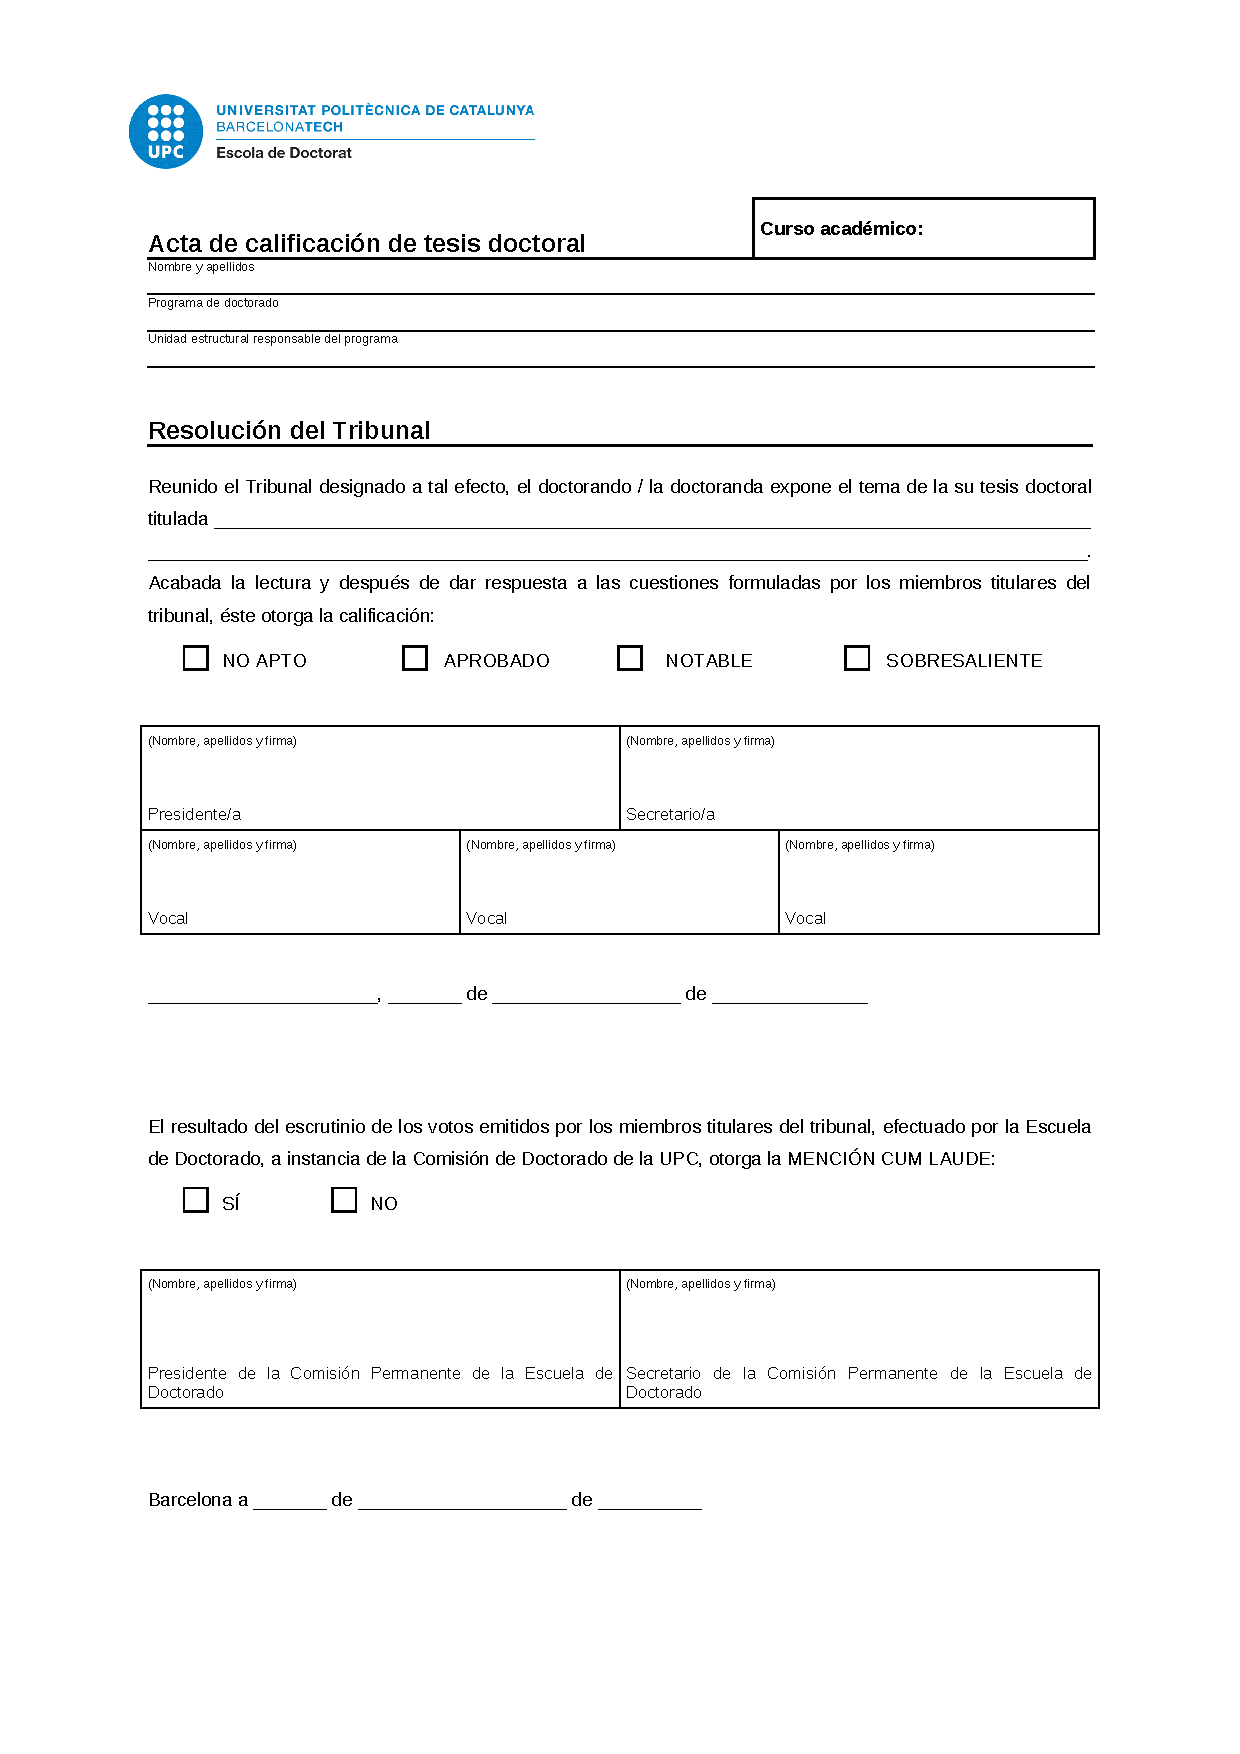
\includepdf[pages={1}]{acta.pdf}

\ifdefineAbstract
 \pagestyle{empty}
 \includeonly{preface/declaration, preface/abstract}
\fi

% ***************************** Chapter Mode ***********************************
% The chapter mode allows user to only print particular chapters with references
% Title, Contents, Frontmatter are disabled by default
% Useful option to review a particular chapter or to send it to supervisior.
% To use choose `chapter' option in the document class

\ifdefineChapter
 \includeonly{Chapter3/chapter3}
\fi

% ******************************** Front Matter ********************************
\begin{document}

\frontmatter

\maketitle

%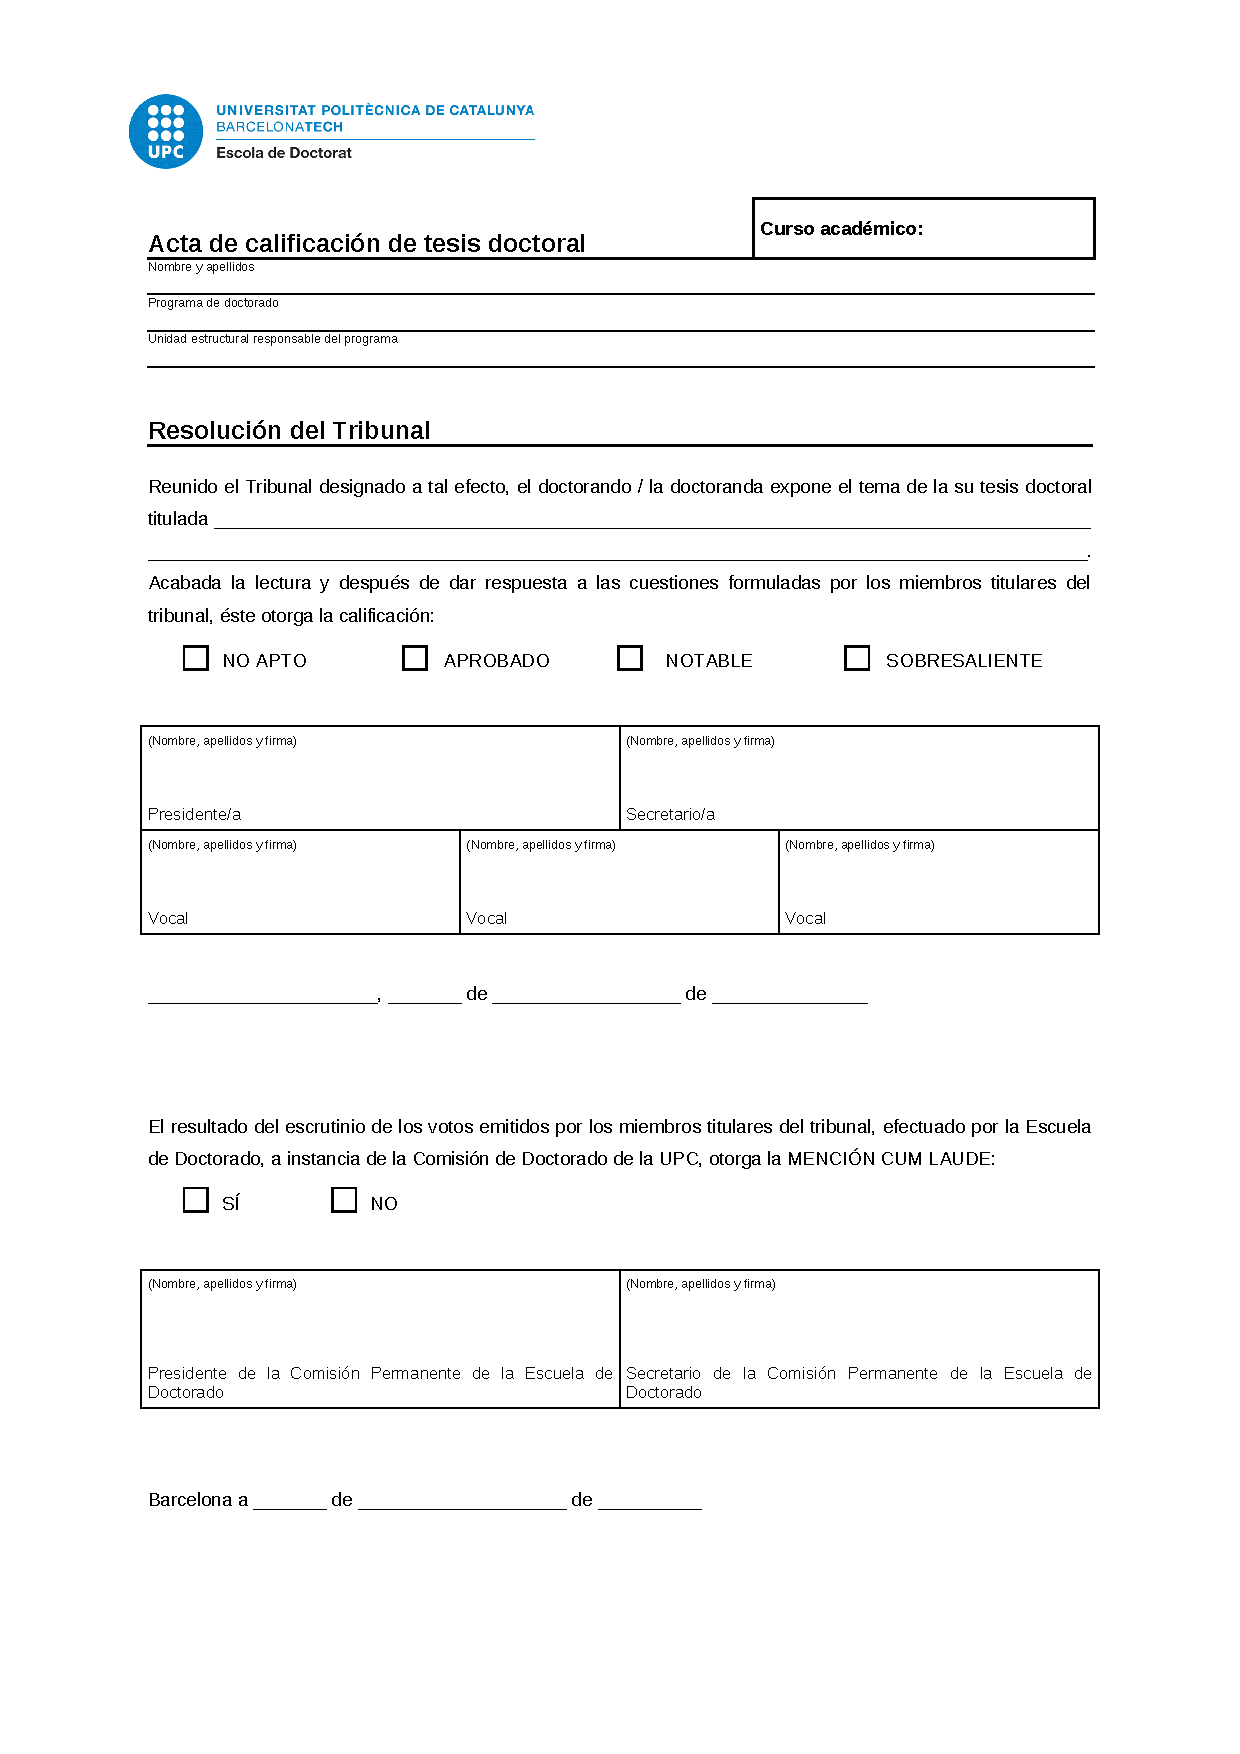
\includegraphics{acta.pdf}
%\clearpage
%\mbox{}
%\clearpage
\newpage\null\thispagestyle{empty}\newpage
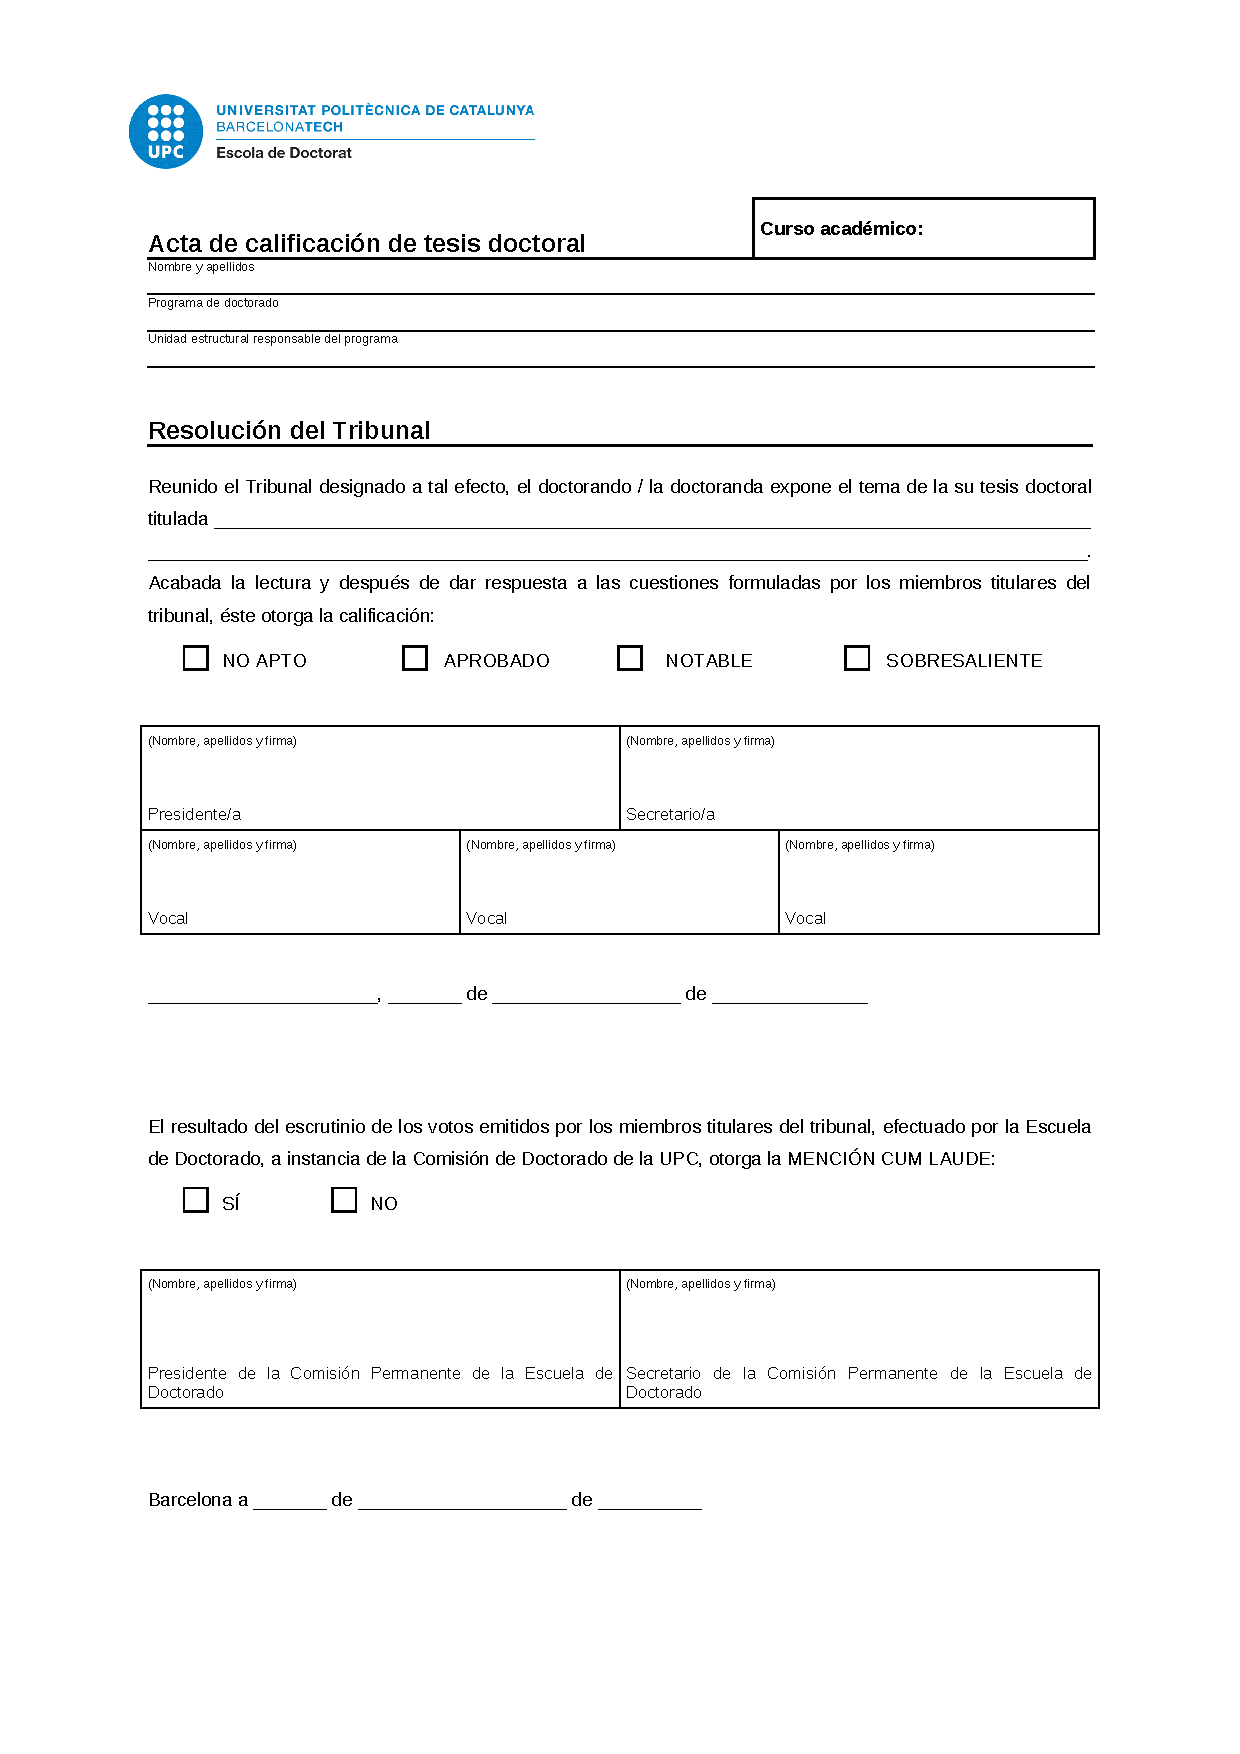
\includepdf[pages=-]{acta.pdf}
\clearpage

\begin{abstract}

\end{abstract}


\begin{dedication}
To my family and friends.

%\vspace*{\fill}
%To think that there at some point in time, someone had the audacity to look
%towards the night sky, where the rest of us remained buffled and silent in
%front of the majesty of the heavens... and blinked in front of the
%incoprehensive vastness of space, and kept at it till all the stars were known.
%\vspace*{\fill}

\end{dedication}

\newpage\null\thispagestyle{empty}\newpage
%

%\clearpage\mbox{}\clearpage
\vspace*{200pt}
\epigraph {I do not know what I may appear to the world, but to myself I seem to have been
only like a boy playing on the sea-shore, and diverting myself in now and then finding a
smoother pebble or a prettier shell than ordinary, whilst the great ocean of truth lay all
undiscovered before me.}{— Isaac Newton}

%\include{Declaration/declaration}

\begin{acknowledgements}
	I would like to extend my gratitude and appreciation to my advisors Dr. Marc
	Casas and Dr. Eduard Ayguad\'{e}, without their patience and guidance this
	thesis would not have been possible. I would also like to thank Dr.
	Cristiano Malossi and Dr. Panagiotis Hadjidoukas from IBM Z\"{u}rich Lab
	who, during the course of our collaboration, gave me valuable feedbacks and
	insights that lead to the success of my work. As well as for their
	hospitality during my month-long stay in Z\"{u}rich that warmed a lone
	traveler's heart.

	It has been a long five-year journey. One does not simply navigate through
	those times alone, not to mention the place I call home is ten thousand km
	away. I want to thank those who were or still are by my side giving me
	support, talking me through things when the getting is tough. My
	appreciation goes to my bestie Kallia, along with Rajiv, Danai, Tomasz and
	David with whom we shared invaluable moments and countless chuckles during
	the good part of my PhD. To Ariel, a close friend that we get along well enough
	to consider sharing an apartment with. To Ilia and Klaudia who we shared a close
	connection despite the little time we spent. Last but not least, a group of
	people of all ages and from all walks of life yet have enough synergy to
	form a close group that I came across over the final months of my PhD: Alex,
	Asaf, Ettore, John "El Cucho" Osorio, Louis "LeDur" Ledoux, Robin and
	Tamara. A group that offers laughters and stories that makes an otherwise
	stressful conclusion of a PhD a lot more entertaining.	

	%This thesis has been supported by the Spanish Government (Severo Ochoa grants
	%SEV2015-0493, SEV-2011-00067), by the Spanish Ministry of Science and
	%Innovation (contracts TIN2015-65316-P), by Generalitat de Catalunya
	%(contracts 2014-SGR-1051 and 2014-SGR-1272), by the RoMoL ERC Advanced
	%Grant (GA 321253) and the European HiPEAC Network of Excellence.  This
	%work was also partially performed under the auspices of the U.S.
	%Department of Energy by Lawrence Livermore National Laboratory under
	%Contract DE-AC52-07NA27344 (LLNL-CONF-689878).
\end{acknowledgements}

\thispagestyle{empty}

% *********************** Adding TOC and List of Figures ***********************

\glsaddall

\tableofcontents

\clearpage
%\printglossary
% \printnomenclature[space] space can be set as 2em between symbol and description
%\printnomenclature[3em]

%\printnomenclature

% ******************************** Main Matter *********************************
\mainmatter

\chapter{Introduction}
\label{chap:introduction}
Modern parallel systems make extensive use of their massive amount of CPU core 
counts or their peripheral accelerators (GPU, FPGA, ASIC etc.). In order to 
effectively parallelize the problem at hand, algorithm designers need to 
meticulously split the problem into smaller chunks that can be executed on the 
individual computational units. \textbf{\textcolor{red}{expansion needed}}

Not all problems are created equal. For some, denoted as \textit{embarrassingly parallel}, 
the task is relatively simple because they can be easily solved in a divide and 
conquer fashion. Each component is inherently independent in that it does not 
require the computational results from its counterparts. 
\textbf{\textcolor{red}{examples, refs}}

Others on the other hand, oftentimes have non-parallelizable sections that 
create interleaving parallel-sequential-parallel patterns during the execution where 
synchronization is required. It is also a commonplace that parallel sections 
possess dependencies in which case communication inevitably occur.
\textbf{\textcolor{red}{examples, refs}}

As peripherals, the various types of accelerators are connected through external 
buses like PCI, NVlink etc. Necessary data has to be transferred from the host 
CPUs to the accelerators before carrying out any meaningful computation. It is 
prominent among iterative-based numerical methods and with the rise of deep 
neural networks.

Synchronization and communication put the involved computational units on hold 
thus impede the execution progress. The scale of the parallel system is the 
primary impact factor of the efficiency of the communication for the following 
reasons.
\begin{itemize}
    \item The physical proximity of the communicating nodes determines the 
        quality of the communication. In a distributed system with nodes scattered 
        at different physical locations, the communication inbalance could create 
        serious bottlenecks.
    \item The need to send data back and forth is alleviated on a shared-memory 
        system where all the computational units have access to entire memory region. 
        Nevertheless, such systems are inherently limited by size. Another type 
        of underlying memory hierarchy is distributed-memory systems where each 
        node is in possess of a portion of the entire memory. The acquisition 
        of contents from other memory regions has to be resolved by passing 
        messages which could raise contention on the bus system.
\end{itemize}
 
\section{Thesis Objectives and Contributions}
This thesis strives to alleviate the communication by reducing either the 
occurrences of communication points or the quantity of data in the domain of 
iterative numerical methods and deep neural networks, while in the meantime 
retaining the quality of the results the algorithms produce. 

\subsection{Communication Reduction in Conjugate Gradient Method}
The conjugate gradient method solves a linear system in an iterative manner. 
Conventionally, synchronization is needed at the end of each iteration in a 
parallel implementation for some bookkeeping tasks such as checking the 
convergence and applying the residual replacement strategy. 
We propose the \emph{Iteration-Fusing Conjugate Gradient} which fuses some of the 
iterations by removing the inter-iteration synchronization points within those fused 
iterations and moving the bookkeeping tasks to the end of the last iteration from the fusion. 
Also we use a task-based parallel programming model to split numerical kernels 
into subkernels to relax data-dependencies. By carrying out these two optimizations, 
our approach allows computations belonging to different iterations to overlap if 
there are no specific data or control dependencies between them.
The main contributions of this approach are:
\begin{itemize}
       \item The Iteration-Fusing Conjugate Gradient (IFCG) approach, which aims 
           at aggressively overlapping different iterations. IFCG is implemented 
           by means of two algorithms: IFCG1 and IFCG2.
       \item A task-based implementation of the IFCG1 and IFCG2 algorithms that 
           automatically overlaps computations from different iterations without 
           the need for explicit programmer specification on what computations should be overlapped.
       \item A comprehensive evaluation comparing IFCG1 and IFCG2 with the most 
           relevant state-of-the-art formulations of the CG algorithm. 
           IFCG1 and IFCG2 provide parallel performance improvements up to 42.9\% 
           and 41.5\% respectively and average improvements of 11.8\% and 7.1\% with 
           respect to the state-of-the-art techniques and show similar numerical stability.
        \item A demonstration that under realistic system noise regimes IFCG 
            algorithms behave much better than previous approaches. IFCG algorithms 
            achieve an average 18.0\% improvement over the best state-of-the-art 
            techniques under realistic system noise regimes.
\end{itemize}

\subsection{Communication Reduction in Training Deep Neural Network Models}
We describe and evaluate a method to accelerate the training of DNNs by reducing the cost 
of data transfers across heterogeneous high-end architectures integrating multiple GPUs. By relying on DNNs 
tolerance to data representation formats smaller than the commonly used 32-bit Floating 
Point (FP) standard~\cite{gupta15, flexpoint17}, we describe how to dynamically adapt 
the size of data sent to GPU devices without hampering the quality of the training process. 
Our solution is designed to efficiently use the incoming bandwidth of the GPU accelerators.
It relies on an adaptive scheme that dynamically adapts the data representation format required 
by each DNN layer and compresses network parameters before sending them over the parallel system.
This scheme enables DNNs training to progress in a similar rate as if the 32-bit FP format was used.
This work makes the following contributions:
\begin{itemize}
    \item It proposes the {\it Adaptive Weight Precision (AWP)} algorithm, which 
        dynamically adapts the numerical representation of DNN weights during training. 
        AWP relies on DNNs' tolerance for reduced data representation formats.  
        It defines the appropriated data representation format per each network layer during  
        training without hurting network accuracy.

    \item It proposes a new {\it Approximate Data Transfer (ADT)} procedure to compress 
        DNN's weights according to the decisions made by the AWP algorithm. 
        ADT relies on both thread- and SIMD-level parallelism  
        and is compatible with architectures like IBM's POWER 
        or x86. ADT is able to compress large 
        sets of weights with minimal overhead, which enables the large performance benefits of our approach.

    \item It evaluates ADT and AWP on 
        two high-end systems: The first is composed of two x86 Haswell multicore 
        devices plus four Tesla GK210 GPU accelerators and the second system integrates two POWER9 chips and four NVIDIA Volta V100 GPUs. 
        Our evaluation considers the Alexnet~\cite{alexnet}, the VGG~\cite{vgg} and the Resnet~\cite{resnet} network models applied to 
        the ImageNet ILSVRC-2012 dataset~\cite{imagenet}.
        Our experiments report average performance benefits of 6.18\% and 11.91\% on the x86 and the POWER systems, respectively.
        Our solution does not reduce the quality of the training process since networks final accuracy is the same as if they had been trained with the 32-bit Floating Point format.
\end{itemize}

\subsection{Communication Reduction in Deep Learning Model Parallelism}


\section{Thesis Structure}

\chapter{Background}
\label{chap:background}
This section provides a description on the state-of-the-art and the current 
challenges presented in the field of parallel computing and deep learning in 
order to grasp the works carried out from this thesis.
Section~\ref{sec:mps} prepares the reader with the acquaintances of the various 
forms of modern parallel systems. Section~\ref{sec:ppm} provides background on 
the parallel programming models on modern parallel systems. Subsequently, 
section~\ref{sec:solvers} and~\ref{sec:dnn} present an introduction to the two 
application domains this work deals with, namely, parallel numerical algorithms 
and DNNs.

\section{Modern Parallel Systems}
\label{sec:mps}
Exascale supercomputers are expected to come into operation near 2020. In order 
to reach that, major improvements need to be achieved including the energy and 
power, memory and storage, concurrency and locality and resiliency~\cite{doe}.  
Nevertheless, the mainstream trend stays with the massive parallelism with 
accelerators approach. This section provides a background on both types of 
systems and an introduction to some major parallel programming models.

With the roll-out of 7 and 5 nm node, the VLSI (very large scale integration) 
manufacturing technology is rapidly approaching its end due to its physical 
limitation. Furthermore, the power and energy consumption, as a consequence the 
heat dissipation, on a modern VLSI chip has become a major limiting factor in 
processor design. All the above impede the efforts to push a single-core 
processor to go faster. In response, industry turns its attention into designing 
multi-core multiprocessor systems which exploit parallelism at the application 
level. Figure~\ref{fig:multicore} illustrates a typical multi-core 
multiprocessor system~\cite{ibm_multicore}. Each of the processors (processor 0 
and 1) packs two separate cores with their own L1 and L2 caches. The two 
processors are connected via a system bus which also connects to the RAM. All 
the cores thus are able to access to the entire memory region. Nonetheless, 
since all the access to the memory and communication among processors are 
conducted on the system bus, the system is limited in its scale in that the 
inevitable contention on the bus system while the number of processors grows 
eventually renders a large-scale system unresponsive.
\begin{figure}[H]
    \centerline{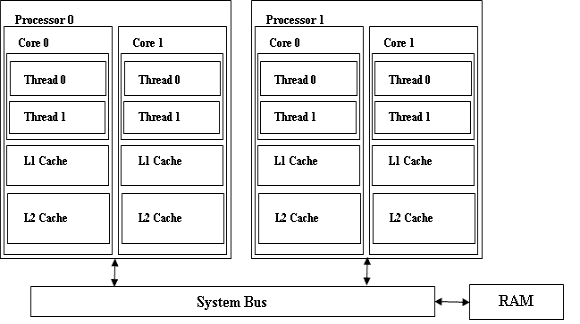
\includegraphics[scale=0.50]{background/figs/multicore_mp_system.png}}
    \caption{A typical chip multithreaded, multi-core, multiprocessor system}
    \label{fig:multicore}
\end{figure}

With the ever-growing demand of computation power, a large amount of such 
processors are grouped close together into a computer cluster with high speed 
interconnection system to further scale the system. All the cores belonging to 
the same node in the cluster shares the resources (memory system, last-level 
cache etc.) whereas cross-node resources are private to their respective nodes.  
This essentially segregates the memory system into various regions not directly 
accessible to all the cores. This type of memory system is known as 
distributed-memory system. Accessing remote contents is possible by sending them 
as message to the requesting node which implies that accessing to different 
memory regions incurs distinct latency.  This offloads the task of ensuring the 
performance of the program to the programmer because careless handling of the 
physical location and topology of the nodes can easily saturate the 
interconnection system and cause different processors to have imbalanced 
accessing time to the same data.

Since the dawn of the artificial intelligence, GPU, due to its immense data 
parallelism capability, has accelerated its transformation from a peripheral 
device used in niche domains to a general-purpose mass adoption. Along with the 
re-configurability of FPGAs and domain-specific ASICs, heterogeneous systems 
contribute to a significant portion of computation power on some modern parallel 
systems. As external devices, to be able to exploit their parallelism, data has 
to be transferred from the CPU to the device and vice versa in the face of any 
synchronization or communication. 

\section{Parallel Programming Models}
\label{sec:ppm}
Parallel programming models can roughly be categorized into two class: one for 
shared-memory systems and the other for distributed-memory systems. The 
classification is due to the distinct ways these models deal with the underlying 
memory system.

\subsection{Shared-Memory Programming Model}
OpenMP~\cite{openmp, OpenMP4.0} is a standard programming model on a 
shared-memory system. It is an application programming interface (API) that 
supports shared memory multiprocessing programming in C, C++, and FORTRAN.

OpenMP (prior to version 3.0) uses a fork-join model for its parallel executions 
as seen in Figure~\ref{fig:fork-join}.
All OpenMP programs begin as a single process: the master thread. The master 
thread executes sequentially until the first parallel region construct is 
encountered. The master thread then creates a team of parallel threads.
The statements in the program that are enclosed by the parallel region construct 
are then executed in parallel among the various team threads. When the team 
threads complete the statements in the parallel region construct, they 
synchronize and terminate, leaving only the master thread~\cite{llnl_openmp}.
\begin{figure}[H]
    \centerline{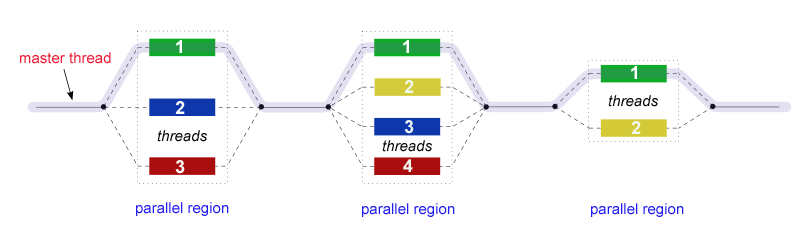
\includegraphics[scale=0.50]{background/figs/fork_join.png}}
    \caption{OpenMP uses a fork-join model}
    \label{fig:fork-join}
\end{figure}

\subsection{Task-based Parallel Programming Model}
A fork-join model creates parallel regions each of which is dedicated to solving 
a specific problem whereas the program logic is executed in sequential on the 
master thread. It introduces inefficiencies because the parallel regions can be 
far between and the sequential execution in-between keeps all the other threads 
idle. 

Task-based parallel programming model sets off to tackle this problem. In a 
task-based approach the problem is ideally re-factorized and decomposed into 
smaller functions called tasks that have clear set of inputs and outputs from 
which data dependencies can be derived unambiguously. Therefore, tasks can be 
launched and executed in parallel as long as they don't have data dependencies 
among each other and hardware resources are available. A dedicated runtime 
system is in charge of building the dependency graph and orchestrating the task 
scheduling. Figure~\ref{fig:task-dependency} illustrates a typical task 
dependency graph which is a DAG (directed acyclic graph) that the runtime system 
uses to check the pending dependencies. There are many task-based parallel 
programming models, the most prominent of which includes the OpenMP (version 3.0 
onwards)~\cite{OpenMP4.0}, Clik++~\cite{clik}, TBB~\cite{tbb} and 
OmpSs~\cite{ompss}.

\begin{figure}[H]
    \centerline{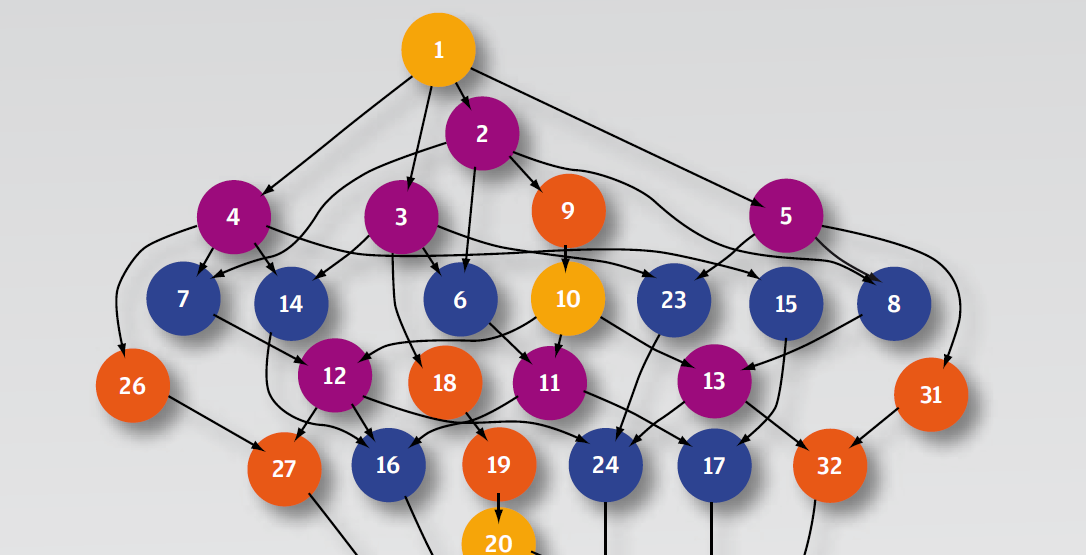
\includegraphics[scale=0.50]{background/figs/starss.png}}
    \caption{A typical task dependency graph}
    \label{fig:task-dependency}
\end{figure}

\subsection{Distributed-Memory Programming Model}
MPI (Message Passing Interface) is the main parallel programming paradigm for 
distributed memory environments. It is a library specification for 
message-passing, proposed as a standard by a broadly based committee of vendors, 
implementors, and users. It primarily addresses the message-passing parallel 
programming model: data is moved from the address space of one process to that 
of another process through cooperative operations on each 
process~\cite{llnl_mpi}.

The MPI interface is meant to provide essential virtual topology, 
synchronization, and communication functionality between a set of processes 
(that have been mapped to nodes/servers/computer instances) in a 
language-independent way, with language-specific syntax (bindings), plus a few 
language-specific features. MPI programs always work with processes, but 
programmers commonly refer to the processes as processors. 

MPI library functions include, but are not limited to, point-to-point 
rendezvous-type send/receive operations, choosing between a Cartesian or 
graph-like logical process topology, exchanging data between process pairs 
(send/receive operations), combining partial results of computations (gather and 
reduce operations), synchronizing nodes (barrier operation) as well as obtaining 
network-related information such as the number of processes in the computing 
session, current processor identity that a process is mapped to, neighboring 
processes accessible in a logical topology, and so on. Point-to-point operations 
come in synchronous, asynchronous, buffered, and ready forms, to allow both 
relatively stronger and weaker semantics for the synchronization aspects of a 
rendezvous-send~\cite{wiki_mpi}.

\section{Numerical Methods For Systems of Linear Equations}
\label{sec:solvers}
Systems of equations are used to represent physical problems that involve the 
interaction of various properties. The variables in the system represent the 
properties being studied, and the equations describe the interaction between the 
variables. The system is easiest to study when the equations are all linear.  
Often the number of equations is the same as the number of variables, for only 
in this case is it likely that a unique solution will exist. Although not all 
physical problems can be reasonably represented using a linear system with the 
same number of equations as unknowns, the solutions to many problems either have 
this form or can be approximated by such a system. In fact, this is quite often 
the only approach that can give quantitative information about a physical 
problem. The problem is to find the vectors of unknown $x$ in $Ax = b$
$$
A=
\begin{pmatrix}
    a_{11}&a_{12}&...&a_{1n}\\
    a_{21}&a_{22}&...&a_{2n}\\
    ...&...&...&...\\
    a_{m1}&a_{m2}&...&a_{mn}\\
\end{pmatrix}
$$
where $x \in \Re^n$, $b \in \Re^m$ and $A \in \Re^m$ x $\Re^n$.

Two classes of numerical methods are available for solving the system:
\begin{itemize}
    \item Direct Methods that provide the exact solution $x$ by a finite 
        sequence of operations.
    \item Iterative Methods that start with a first approximation $x^{(0)}$ and 
        compute in an iterative manner a sequence of approximations $x^{(i)}$, 
        in the hope to obtain increasingly better results, without ever reaching 
        $x$.
\end{itemize}

\subsection{Direct Methods}
A common way to obtain the exact numerical results of systems of linear 
equations is using matrix factorization.

LU factorization of a matrix is the factorization of a given square matrix into 
two triangular matrices, one upper triangular matrix and one lower triangular 
matrix, such that the product of these two matrices gives the original matrix.  
The LU factorization method comes handy whenever it is possible to model the 
problem to be solved into matrix form. Conversion to the matrix form and solving 
with triangular matrices makes it easy to do calculations in the process of 
finding the solution~\cite{mc, nla}.

For $$ A=
\begin{pmatrix}
    a_{11}&a_{12}&a_{13}\\
    a_{21}&a_{22}&a_{23}\\
    a_{31}&a_{32}&a_{33}\\
\end{pmatrix} $$ we have
$$ L=
\begin{pmatrix}
    1      &  0       &  0  \\
    l_{21} &  1       &  0  \\
    l_{31} &  l_{32}  &  1  \\
\end{pmatrix} $$ and $$ U=
\begin{pmatrix}
    u_{11} &  u_{12}  &  u_{13}  \\
    0 &  u_{22}  &  u_{23}  \\
    0 &  0  &  u_{33}  \\
\end{pmatrix} $$ such that $A = LU$. The system of equations $Ax = b$ can thus 
be solved by the following steps:
\begin{enumerate}
    \item Factorize the matrix $A$ so that $LUx = b$
    \item Solve the equation $Ly = b$ for $y$ by forward substitution
    \item Solve the equation $Ux = y$ for $x$ by backward substitution
\end{enumerate}

Cholesky factorization is a faster method if the matrix $A$ is symmetric 
positive-definite. In which case $A$ can be factorized into $A = LL^T$ where 
where $L$ is a lower triangular matrix with real and positive diagonal entries, 
and $L^T$ denotes the transpose of L~\cite{nla}.

\subsection{Iterative Methods}
In the absence of rounding errors, direct methods would yield an exact solution 
yet iterative methods are indispensable when facing linear problems involving a 
large number of variables (in the order of millions or more), where direct 
methods would be prohibitively expensive even with the best available computing 
power~\cite{nla}. 

Krylov methods are among the most successful iterative methods and see a wide 
application in numerical linear algebra. Krylov subspace methods solves a linear 
system $Ax = b$ by forming a basis of the sequence of successive matrix powers 
times the initial residual, \{$b, Ab, A^2b, \ldots, A^mb$\}. The approximations 
to the solution are then formed by minimizing the residual over the subspace 
formed. The prototypical method in this class is the conjugate gradient method 
(CG)~\cite{cg} which assumes that the system matrix $A$ is symmetric 
positive-definite. For symmetric (and possibly indefinite) $A$ one works with 
the minimal residual method (MINRES)~\cite{minres}. In the case of not even 
symmetric matrices methods, such as the generalized minimal residual method 
(GMRES)~\cite{gmres} and the biconjugate gradient method (BiCG)~\cite{bicg}, 
have been derived.

\section{Deep Supervised Learning and Its Parallelization}
\label{sec:dnn}
Deep learning uses multi-layer neural networks to carry out wide range of tasks 
such as image recognition~\cite{alexnet},  video 
classification~\cite{video_class}, various NLP (natural language processing) 
tasks~\cite{nlp0, nlp1, nlp2, nlp3} and art generation~\cite{gan, can} just to 
name a few. A neural network consists of layers of neurons which are themselves 
a mathematical model of a linear classifier. Figure~\ref{fig:perceptron} depicts 
the inner workings of a neuron. The neuron takes a vector of inputs $x$, first 
calculate its weighted sum $y = \sum_{i=1}^{n} x_i w_i$ and apply a non-linear 
step function $o = \delta(y)$. An MLP (multi-layer perceptron) is thus comprised 
of multiple layers each of which is constituted of multitudes of neurons with 
their respective set of weights per input.
\begin{figure}[H]
    \centerline{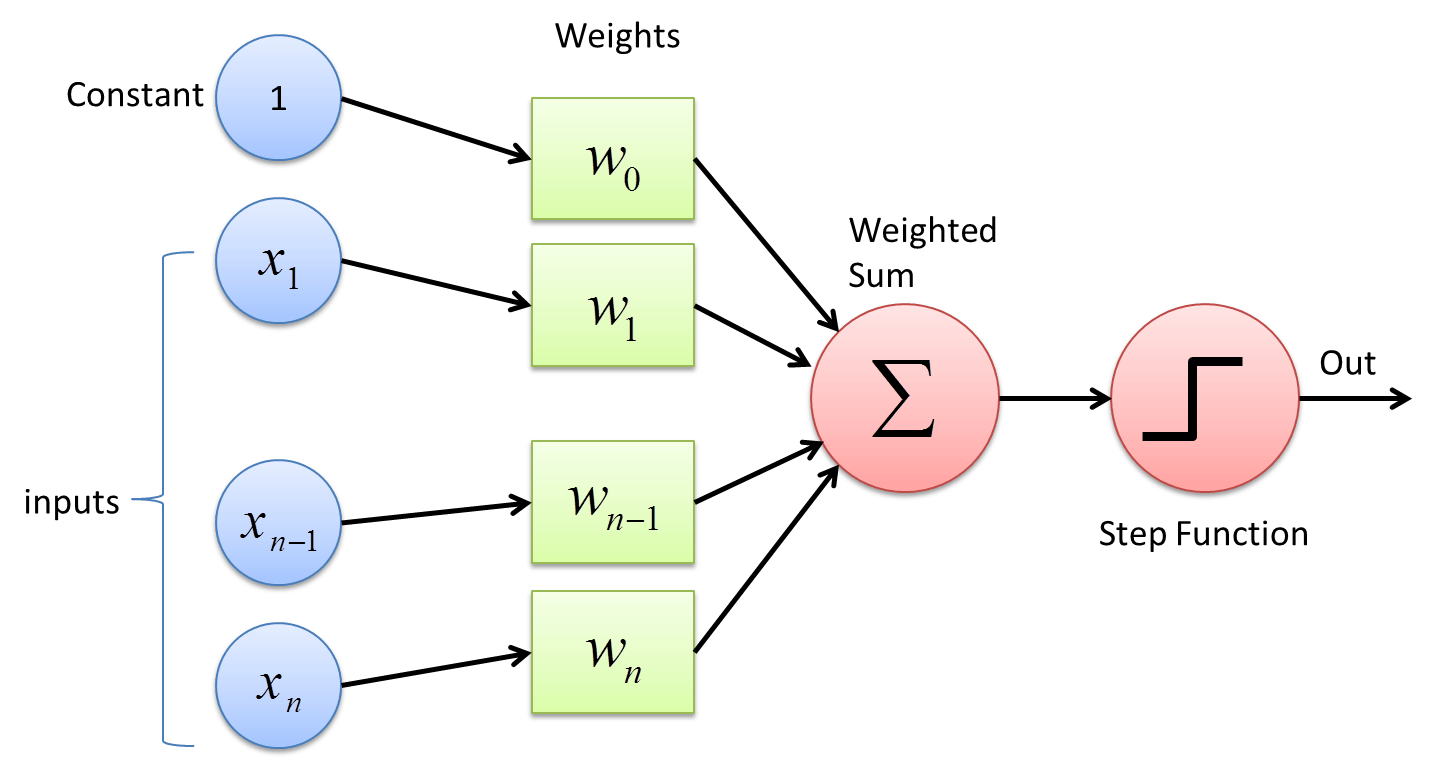
\includegraphics[scale=0.25]{background/figs/perceptron.png}}
    \caption{The workings of a neuron}
    \label{fig:perceptron}
\end{figure}

This thesis has its focus on one particular branch of the deep learning, namely, 
deep supervised learning. It utilizes a MLP (multi-layer perceptron) or CNN 
(convolutional neural network) to learn a function that maps an input to an 
output based on example input-output pairs. It infers a function from labeled 
training data consisting of a set of training examples. The dataset in 
supervised learning are a pair of input and a ground truth (the desired output).
The neural network learns by adjusting all the weights from each neuron 
according to its gradient $w' = w - \mu \Delta w$ to the lost yielded by a loss 
function that measures the difference of the output of the neural network and 
the ground truth. A typical loss function is MSE (mean square error), cross 
entropy etc.

\subsection{Parallelism in Deep Learning}
Effectively training a neural network demands an immense amount of data. This 
inevitably raise the need for parallelization. Currently, there are two 
paradigms:
\begin{itemize}
    \item Data parallelism aims to run the training on data batches 
        simultaneously.
    \item Model parallelism aims to split the neural network itself to available 
        computation units.
\end{itemize}

\subsubsection{Data Parallelism}
The most common way in the data parallelism paradigm is the use of a parameter 
server~\cite{pserver}. The dataset is split into data shards that are 
consequently fed to each and every computation units respectively. The 
parameters (weights $w$, biases $b$ etc.) are stored separately in dedicated 
units called parameter servers. At the beginning of each batch of the training, 
all the computation units involved in the training request a up-to-date copy of 
the parameters from the servers. They carry on with the training and at the end 
of the batch send their respective gradient $\Delta w$, $\Delta b$ back to the 
servers. The servers then are responsible for updating the parameters with 
regard to the gradients. Figure~\ref{fig:pserver} illustrates a schematic of two 
parameter servers and three trainers.
\begin{figure}[H]
    \centerline{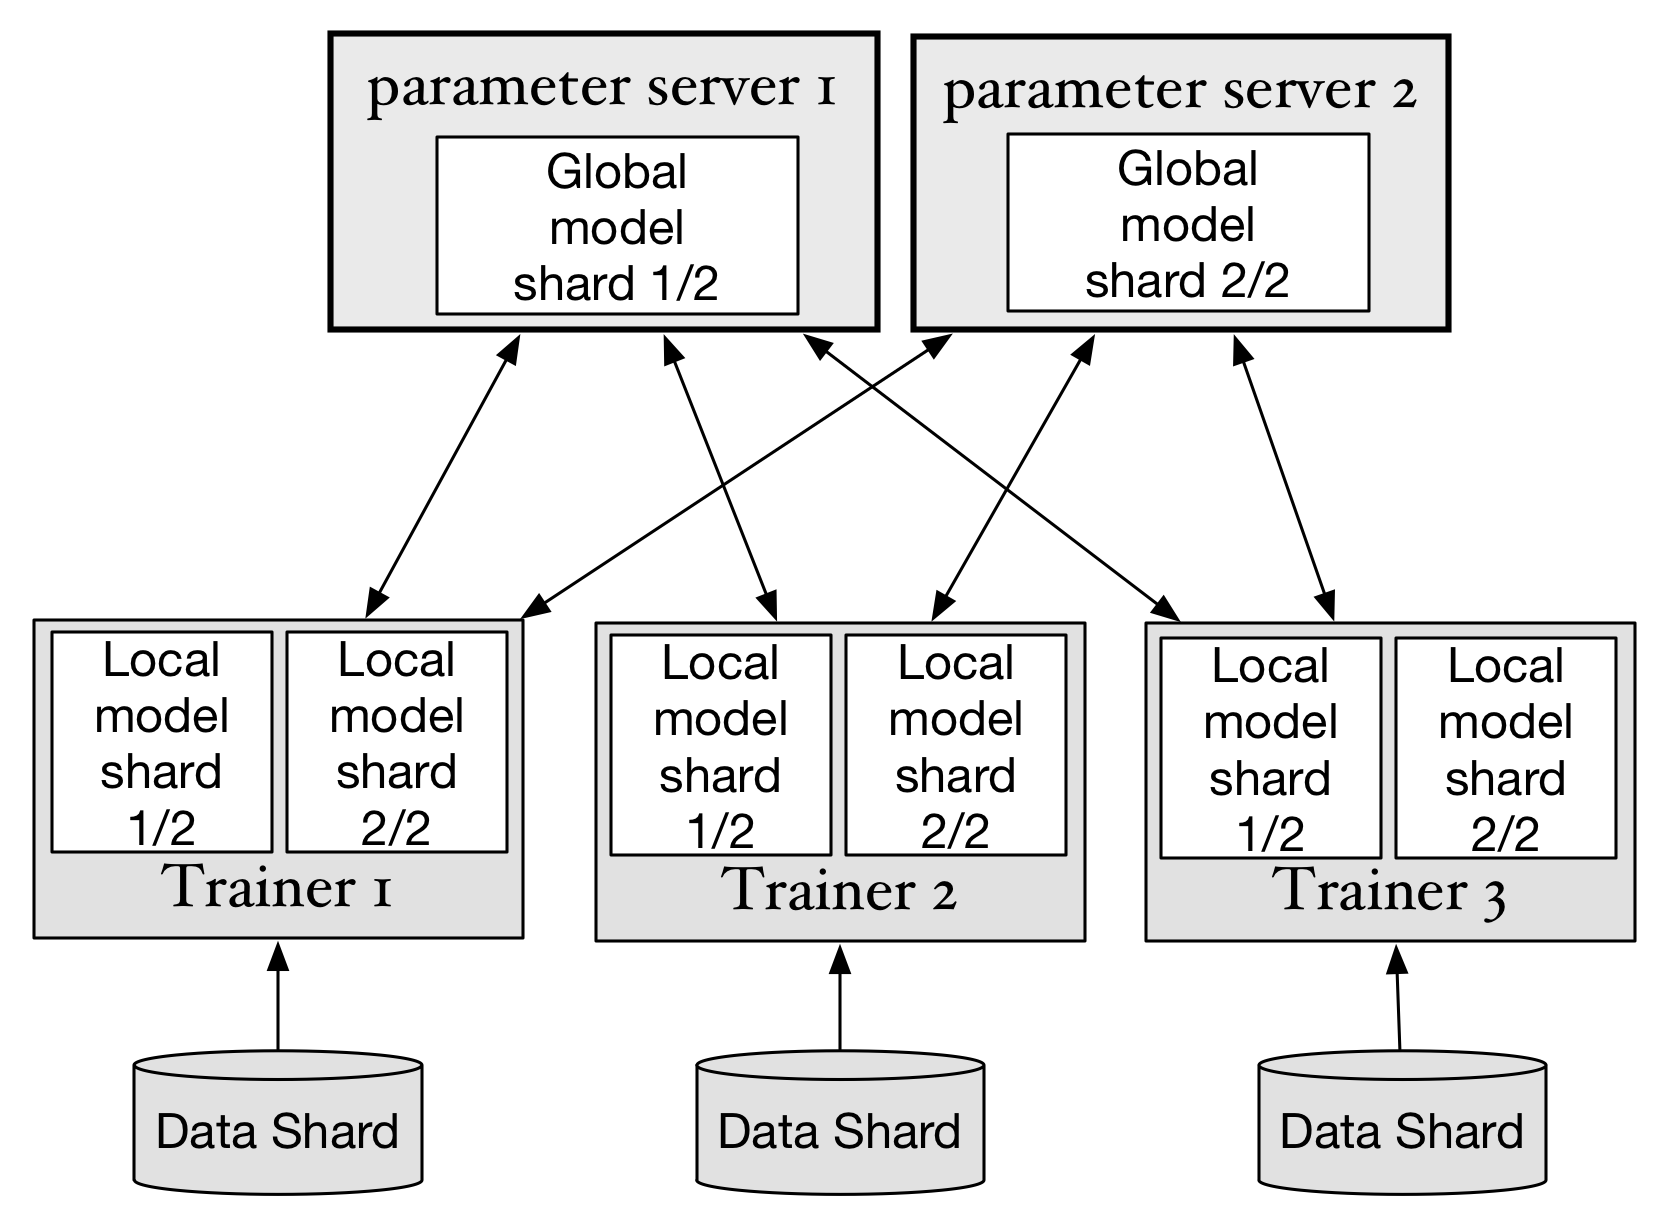
\includegraphics[scale=0.40]{background/figs/data_parallelism.png}}
    \caption{Two parameter server and three trainers}
    \label{fig:pserver}
\end{figure}

\subsubsection{Model Parallelism}
Model parallelism is also called network parallelism. It can be seen as a 
orthogonal to data parallelism. This strategy divides and distributes part of 
the network to different machines. Figure~\ref{fig:model} shows the difference 
between data and model parallelism. Model parallelism is suitable for models 
that are too large to fit into one machine but this comes at a cost of incurring 
additional communication during one batch of training~\cite{model0}.
\begin{figure}[H]
    \centerline{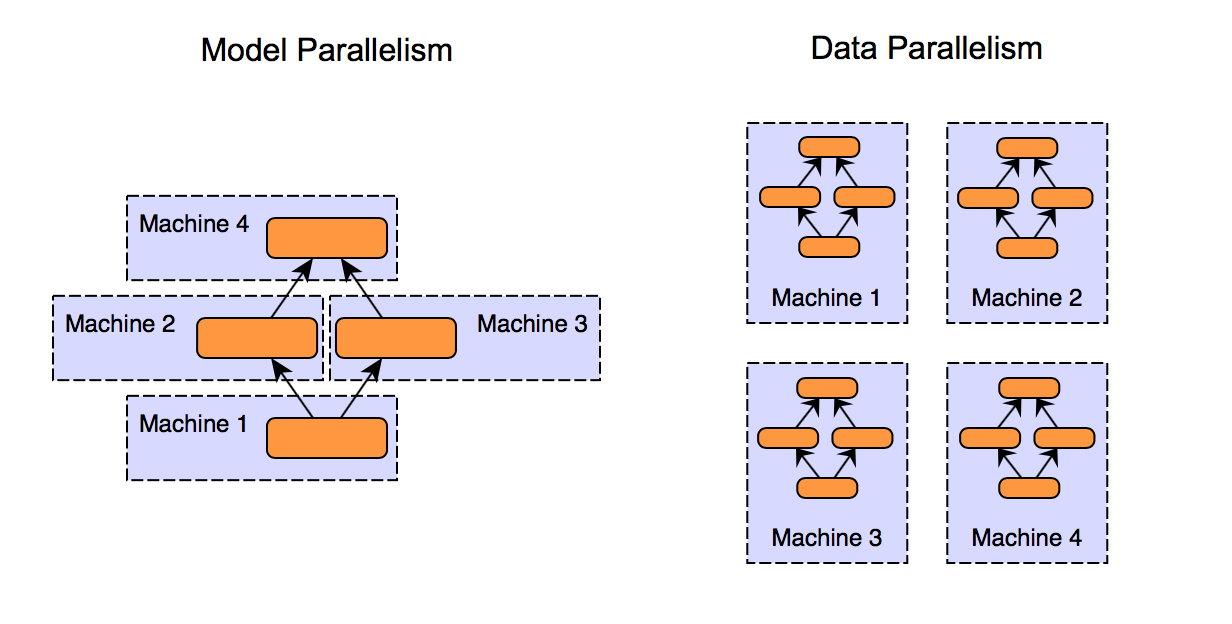
\includegraphics[scale=0.60]{background/figs/model_parallelism.png}}
    \caption{The difference between data and model parallelism}
    \label{fig:model}
\end{figure}

Nevertheless, the DNN architecture creates layer interdependencies, which, in 
turn, generate communication that determines the overall performance. Fully
connected layers, for instance, incur all-to-all communication (as opposed to 
allreduce in data parallelism), as neurons connect to all the neurons of the 
next layer~\cite{model1}.


\chapter{Experimental Setup}
\label{chap:methodology}

In this Chapter we describe the hardware and software platforms used for the experimental
evaluation of this work.  In this work we assume that we work with parallel workloads that
are implemented with a programming model that allows dynamically controlling its
concurrency level.  Applications should also be able to be decomposed into concurrent
tasks.  The underlying hardware platform should offer the ability to impose user defined
power caps, at least per each socket (such as Intel CPU models that are equally or older
than the Sandy Bridge family of processors).  Moreover, older CPU models do not
demonstrate notable manufacturing variability.
We also assume the presence of a workload manager to manage running applications on an 
HPC cluster.   

\section{Hardware Platforms} 
\label{sec:platforms}
For our experimental evaluation we use two distinct HPC
clusters, the MareNostrum III supercomputer at Barcelona Supercomputing Center and the
Catalyst and Quartz clusters at Lawrence Livermore National Lab.  Marenostrum III is one
of Europe's largest supercomputers and represents the state-of-the-art in production
environments in HPC.  Our initial evaluation of the PARSECSs is conducted on MareNostrum
III, however, since it's a large production machine, access to specific MSR registers,
required for monitoring and capping power on Intel chips, is restricted.  For this reason
we also use the Catalyst and Quartz cluster, where MSRs are accessible by the user through
special kernel modules. 

\begin{itemize}
	\item \emph{MareNostrum III}: It consists of 3,056 compute nodes in total. Each node is
IBM System X server iDataPlex dx360 M4, composed of two 8-core Intel Sandy Bridge
processors E5-2.60Hz, 20MB of shared last-level cache. There are eight 4GB DDR3 DIMM's
running at 1.6GHz (a total of 32GB per node and 2GB per core). 

	\item \emph{Catalyst}: The Catalyst cluster~\cite{llnlconfluence} consists of 324 NUMA
nodes, each with two 12-core Intel Xeon E5-2695v2 sockets and equipped with 128GB of main
memory.  It can reach a peak performance of 149.3 PFLOPS.  Access to MSR counters is
granted to normal users through a kernel module.  We use 128 of these nodes (256 sockets)
in our experiments, which totals to 3,072 cores.

	\item \emph{Quartz}: The Quartz cluster~\cite{llnlconfluence} consists of 2,634 NUMA
nodes, each with two 16-core Intel Xeon E5-2695v4 sockets and equipped with 128GB of main
memory.  It can reach a peak performance of 3,251.4 PFLOPS.  For our experiments we use We
use 128 of these nodes (256 sockets) in our experiments (4,096 cores in total).  As with
the case of Catalyst, access to the RAPL interface is granted through a kernel module.
This is a larger production machine we use to gather application execution traces and later
use in our workload manager simulator.

\end{itemize}

\section{Software Stack}

\subsection{Runtime System}
We use the OpenMP 4.0 standard to implement the PARSECSs benchmark suite.  We make use of
the Nanos++ OpenMP runtime system (version 0.8a).  Because of it's modular design it is
ideal to expand it's functionality and offers all OpenMP 4.0 features along with some
experimental ones.  Note that we only use the standard OpenMP 4.0 features in our
implementation.  We also use Nano++ for developing our power-aware runtime approach.
Nanos++ is coupled with the Mercurium source-to-source compiler (version 1.99), and gcc
4.7 as the back-end compiler.  
%To analyze the behavior of the \PARSEC{} benchmark suite (version 3.0), we use the Extrae
%instrumentation package~\cite{Labarta2006} (version 2.5) and the Paraver trace
%viewer~\cite{Labarta2006} (version 4.5). 
%We run all benchmarks using their respective native inputs as described in Table~\ref{tab:parsec}. 

\subsection{Analysis tools and Power Capping Framework}
We use a number of tools to perform various types of analyses on our benchmarks.  We use
the Extrae instrumentation package~\cite{Labarta2006} (version 2.5) and the Paraver trace
viewer~\cite{Labarta2006} (version 4.5) to analyze and compare the PARSEC and PARSECSs
benchmark suites.
 

\textit{Performance and Power Monitoring} 
Our methodology requires to monitor performance counters plus power consumption rates.  We
use \textit{perf} version 3.10 and \textit{mpstat} version 10.5.1 for monitoring
architectural and core component activity.  For measuring power and enforcing power limits
we use Intel's RAPL registers, which expand typical hardware counters, offering precise
readings on power consumption and temperature, as well as offering the functionality to
constrain core power consumption to a certain limit.  On Sandy and Ivy Bridge CPUs, these
special registers are accessible per socket, but on newer architectures like Haskwell,
they offer the same features per core.  We implement a daemon built on top of
\textit{libmsr}~\cite{libmsr}, which is a user friendly framework for accessing RAPL
registers safely from user space, through a special kernel module.  Our study focuses on
the variability on processors.  In our experiments we measured variance in DRAM power
consumption of less than 1\% (measured using the RAPL interface), among different
sockets when running the same benchmark.  For this reason, we only report the power 
consumption of processors.  We use the same framework for power capping sockets on
Catalyst and Quartz.  These power caps are enforced at hardware level by reducing the 
effective frequency of all cores, to match the requested power budget.
The user can specify a time window and a maximum average power for that window.
The processor guarantees that it will not exceed this average.
Intuitively, longer windows may allow better performance
for applications that utilize the CPU in bursts; if the burst
exceeds the window size, the processor will have to be
throttled.

The sample rate is 100ms for power monitoring and 1s for performance counters.  Although
we are able to monitor an applications real power consumption on a finer grain, our
predictions are limited to 1s granularity, since they depend on the performance counter
data collected at the coarser granularity.

\section{Workload Manager Simulator}
\label{sec:simulator}
For testing our scheduling policies, we implement a discrete event simulator, and
implement our scheduling policies on top of it.  Although there already exist workload
manager simulators for SLURM \cite{slurm_sim} and Flux \cite{flux_sim}, they do not model
power.  Moreover, these simulators also require tracing the applications.  We found it to
be more practical to implement our own to better control what traces need to be generated
and how power is to be handled and modeled. 

The simulator  requires all jobs to be first executed on the physical hardware
to gather performance and power profiles,  which are then used to simulate
their execution under different scheduling schemes. The performance and power
profiles are referred to as traces in this document.  They track performance
and power information over time, throughout a job's execution.  These traces
are different to job queues' traces, which contain information on the time a
job is issued, scheduled and completed, as well as which resources were
allocated for its execution.  Idle power is modeled as the average power consumed by each
socket, as measured on the actual hardware.  Using a simulator allows us to
rapidly test and evaluate new policies without any accuracy loss since the
simulations are led by power traces obtained from real parallel executions.
Our design allows the user to implement scheduling policies using python
scripts.  In our setup we implement SLURM's \cite{slurm_02} default job
scheduling policy, since it's the de-facto resource management tool on
production clusters.  The additional policies suggested by this work expand the
functionality of SLURM's default scheduler with power- and
variability-awareness.

\subsubsection{Validation of Workload Manager Simulator}
To validate the simulator we run a small scale experiment using 8 nodes (16
sockets) on Quartz.  The workload we use consists of a mix of a 100 instances
of the PARSECSs benchmarks.  Each instance is a single socket job and is
randomly chosen out of the total 10 PARSECSs benchmarks.  We run a bash script
that periodically issues 10 instances (every 60s) until all the job instances
are issued.  Then, it waits for all jobs to finish execution.  We generate a
trace with the timestamp of when every job was issued and on which node it was
run on.  We also keep track of the total time it takes for all the jobs to
complete along with the total energy the sockets consumed (including idle time).        

We then use the simulator to repeat the experiment and reproduce the results measured on
the actual machine.  We use the same set of nodes and 100 instances.  
%The simulator requires application traces of the applications run on all sockets.  
We run all PARSECSs
applications on all 16 sockets to gather the traces and power profiles (on a different run 
from the original experiment described in the previous paragraph).  Then we issue the same
100 jobs again, this time on the simulator, at the same intervals as with the original run
on the actual machine.  The simulator will also use the workload trace to get the socket each
job run on, and try to replicate the same socket to job allocation, if possible.
This way, it tries to essentially recreating the same scheduling decisions SLURM took on the actual machine.
When all jobs finish execution, we measure the total execution time and energy
consumption.

Comparing total execution time and energy consumption between the two experiments shows
that the simulator is 1.6\% slower than the actual execution on the cluster.  Moreover,
the jobs' total power consumption is higher on the simulator by 1.1\%.  These results
show that our simulator has very good accuracy and the results discussed in Section 
\ref{chap:power_aware_job_scheduling} are representative of the impact our scheduling
policies would have on the actual machine.

\begin{table}
        \centering
        \caption{Benchmark training set for PMC-based power prediction model.}
        \label{tab:training_set}
				\def\arraystretch{1.5}%
				\begin{tabular}{ | c | m{12cm} | }
                \hline
                \textbf{Benchmark} & \textbf{Description} \\
                \hline
                \hline
                cholesky & cholesky factorization kernel \\
                \hline
                knn & K-nearest neighbours kernel \\
                \hline
                matmul & Floating point matrix multiplication kernel \\
                \hline
                md5 & MD5 message-digest algorithm \\
                \hline
                prk2\_stencil & Tests the efficiency with which a space-invariant symmetric filter (stencil) applies to images \\
                \hline
                qr\_tile & Tiled QR factorization kernel \\
                \hline
                sparseLU & Sparse LU factorization kernel\\
                \hline
                stap & Space-Time Adaptive Processing for radar detection of an objects position \\
                \hline
                symmatinv & Symmetric matrix inversion kernel \\
                \hline
                vector-redu & Computes the sum of the elements of a vector \\
                \hline
                mem\_bench & A micro-benchmark that stretches different memory levels \\
                \hline
        \end{tabular}
%	\vspace{-.5cm}
\end{table}


\section{Benchmark Applications}
\subsection{Prediction Model Training}
To train our models we use a set of small kernel and micro-benchmarks, listed in
Table~\ref{tab:training_set}, that capture different behaviors.  In addition to these
kernels, we design a microbenchmark that stresses each level of the memory hierarchy, in
order to measure the impact that each cache level has on power consumption.  Our set
consists of kernel applications which are representative HPC workloads, however often
larger and more exhaustive set of benchmarks are selected for training
\cite{Bertran:2012:SEC:2457472.2457499}.  Although larger sets can give better results, by
capturing a wider variety of application behaviors, we demonstrate that our set provides
comparable results, while it's easy to deploy.  In comparison, Bertran et. al
\cite{Bertran:2012:SEC:2457472.2457499} use a large set of 100 micro-benchmarks, fine
tuned to the underlying architecture.  This set would be ideal for our prediction models
as well, however it is not portable and requires significant effort and understanding of
the underlying architecture, which makes its deployment challenging.

\begin{table}
        \centering
        \caption{NAS Multi-Zone benchmarks are multinode applications that use both MPI and OpenMP
		to express parallelism.  MPI is used for inter-node communication and OpenMP is used 
		for intra-node parallelizations of loops.}
        \label{tab:nas_mz_set}
				\def\arraystretch{1.5}%
				\begin{tabular}{ | c | m{12cm} | }
                \hline
                \textbf{Benchmark} & \textbf{Description} \\
                \hline
                \hline
                BT-MZ & Block Tri-diagonal solver. The workload consists of a mesh, unevenly divided among processes. \\
                \hline
                LU-MZ & Lower-Upper Gauss-Seidel solver. The workload consists of a mesh, evenly divided among process. \\
                \hline
                SP-MZ & Scalar Penta-diagonal solver. The workload consists of a mesh, evenly divided among processes. \\
                \hline
        \end{tabular}
%	\vspace{-.5cm}
\end{table}



\subsection{Runtime and Job Scheduler Evaluation Benchmarks}
\label{sec:benchmarks}
To evaluate the runtime and job scheduling policies considered in this thesis, we use the
 PARSECSs benchmark suite, which we developed after the PARSEC benchmark suite (further
described in Section \ref{sec:parsec}).  The PARSECSs benchmark suite consists of emerging
workloads for shared memory architectures, representative of applications run on typical
HPC systems.  Our implementations use the OmpSs/OpenMP 4.0 programming model, which allows
us to use current and emerging realistic workloads under a sophisticated programming
environment.  This is essential for evaluating our runtime solution for mitigating
manufacturing variability and improving the energy efficiency of the programming model, as the
original PARSEC suite is implemented in Pthreads, and only a couple of them use OpenMP 3.0
constructs, such as parallel loops.  Using a model like OmpSs/OpenMP 4.0, allows us to
easily modify and test our runtime approach without the need to re-implement our methodology for every
benchmark using the Pthreads model.  Moreover, using tasks and dataflow relations allows
us to express more complex parallelization strategies, that are not possible to implement
with the typical fork-join model of Pthreads and OpenMP 3.0.  This allows us to evaluate
our proposal using applications that better represent contemporary parallel workloads.
We discuss our implementations of the PARSECSs in more detail in Chapter
\ref{chap:task_based_benchmarks}.  

In the case of the job scheduling techniques, we use the PARSECSs
as our set of single socket parallel jobs.  However,  multi-node jobs are also common in HPC
environment.  For this reason we expand our benchmark set with the
MPI+OpenMP versions of the NAS multi-zone benchmarks ~\cite{Jin:2006:PCM:1143496.1143503} (NAS-MZ), posing
as our multi-node jobs.  The NAS-MZ benchmarks are described in table \ref{tab:nas_mz_set}. 
%are also a well known set of kernel applications that can run on a large set of nodes, often used in HPC.  
The multi-node jobs
run with different configurations for 8, 16 and 64 MPI processes, where each process runs
on a single socket.  All instances and processes run on 16 cores, with the exception of
\textit{facesim} (8 cores), \textit{fluidanimate} (8 cores), \textit{lu-mz\_D.8} and
\textit{lu-mz\_D.8} (1 core per MPI process).  Our diverse set of applications can run
from a single core up to 768 cores, for the larger MPI codes.  We run all benchmarks 5
times and report median values.  This is done to minimize the impact of noise or unrelated
to manufacturing variability inference in our experiments.  However, note that variation
in performance and power observed in all of our experiments were below 2\% (when repeating 
the same run on the same socket).

%\subsection{The PARSEC benchmark suite}
%
\begin{table*}[!t]
	\centering
	\scriptsize
	\caption{\PARSEC{} Benchmark Suite}
	\begin{tabular}{|l|p{6cm}|p{3cm}|p{1cm}|}
	\hline
	\textbf{Benchmark} & \multicolumn{1}{|c|}{\textbf{Description}} & \multicolumn{1}{|c|}{\textbf{Native input}} & \multicolumn{1}{|c|}{\textbf{LOC}}\\
	\hline \hline
	blackscholes & Intel RMS benchmark. It calculates the prices for a portfolio of European options analytically with the Black-Scholes partial differential equation (PDE). & 10,000,000 options & 404 \\ \hline
	bodytrack & Computer vision application which tracks a 3D pose of a marker-less human body with multiple cameras through an image sequence. & 4 cameras, 261 frames, 4,000 particles, 5 annealing layers & 6,968\\ \hline
	canneal & Simulated cache-aware annealing to optimize routing cost of a chip design. & 2,500,000 elements, 6,000 temperature steps & 3,040\\ \hline
	dedup & Compresses a data stream with a combination of global compression and local compression in order to achieve high compression ratios. & 672 MB data & 3,401\\ \hline
	facesim & Intel RMS workload which takes a model of a human face and a time sequence of muscle activation and computes a visually realistic animation of the modeled face. & 100 frames, 372,126 tetrahedra & 34,134\\ \hline
	ferret & Content-based similarity search of feature-rich data such as audio, images, video, 3D shapes, etc. & 3,500 queries, 59,695 images database, find top 50 images & 10,552\\ \hline
	fluidanimate & Intel RMS application uses an extension of the Smoothed Particle Hydrodynamics (SPH) method to simulate an incompressible fluid for interactive animation purposes. & 500 frames, 500,000 particles & 2,348\\ \hline
	freqmine & Intel RMS application which employs an array-based version of the FP-growth (Frequent Pattern-growth) method for Frequent Itemset Mining (FIMI). & 250,000 HTML documents, minimum support 11,000 & 2,231\\ \hline
	raytrace & Intel RMS workload which renders an animated 3D scene. & 200 frames, 1,920$\times$1,080 pixels, 10 million polygons & 13,751\\ \hline
	streamcluster & Solves the online clustering problem. & 200,000 points per block, 5 block & 1,769\\ \hline
	swaptions & Intel RMS workload which uses the Heath-Jarrow-Morton (HJM) framework to price a portfolio of swaptions. & 128 swaptions, 1,000,000 simulations & 1,225\\ \hline
	vips & VASARI Image Processing System (VIPS), which includes fundamental image processing operations. & 18,000$\times$18,000 pixels & 127,957\\ \hline
	x264 & H.264/AVC (Advanced Video Coding) video encoder. & 512 frames, 1,920$\times$1,080 pixels & 29,329\\ \hline 
	\end{tabular}
	\label{tab:parsec}
	\vspace{1cm}
\end{table*}

With the prevalence of many-core processors and the increasing relevance of application domains that do not belong to the traditional HPC field, 
comes the need for programs 
representative of current and future parallel workloads. 
The \PARSEC{}~\cite{Bienia:PhD2011} features state-of-the art, 
computationally intensive algorithms and very diverse workloads from different areas of computing.
\PARSEC{} is comprised of 13 benchmark programs. 
The original suite makes use of the Pthreads parallelization model for all these benchmarks, 
except for \texttt{freqmine}, which is only available in OpenMP. 
The suite includes input sets for native machine execution, which are real input sets.
Table~\ref{tab:parsec} describes the different benchmarks included in the suite along with their respective native input and the lines of code 
(LOC) of each application.
We apply tasking parallelization strategies to 11 out of its 13 applications: \texttt{blackscholes}, \texttt{bodytrack}, \texttt{canneal}, \texttt{dedup}, \texttt{facesim}, \texttt{ferret}, 
\texttt{fluidanimate}, \texttt{freqmine}, \texttt{streamcluster} and \texttt{swaptions} and \texttt{x264}. 
We leave 2 applications out of this study: \texttt{raytrace} and \texttt{vips}.
\texttt{Vips} is a domain specific runtime system for image manipulation. 
Since vips is a runtime itself, it is not reasonable to implement it on top of another runtime system. 
Therefore we do not include this code in our evaluations. 
\texttt{Raytrace} code has the same extension as 
\texttt{ferret}, \texttt{facesim} and \texttt{bodytrack} and the same parallel model as \texttt{blackscholes}~\cite{Cook:2013:HEC:2508148.2485949}.
Therefore, since it does not offer any new insight, we do not consider the \texttt{Raytrace} code in this work.
 
We have a preliminary task-based implementation of the \texttt{x264} encoder, which scales up to 14x on a 16-core machine, the same as the Pthreads version.  
Since we just emulate the same parallel model as the original Pthreads version and obtain the same performance, we do not include this code in the results Section as it provides no insight.





\subsection{Job Scheduler Workload Generation}
\label{sec:cluster_traffic}
Typically workload manager schedulers are evaluated using workload traces from the job
queues of actual HPC clusters \cite{Etinski2012615,FEITELSON20142967}.  However, in our
case this is not applicable, since these type of traces do not contain information on
power and manufacturing variability.  Moreover, we are not able to create a job queue trace
out of the clusters we have access to, since reading performance counters such as the RAPL
interface requires root access.  This is not an option for us on these production
machines.  For these reasons we generate our own cluster workload combining single- and
multi-node applications, so that we can measure the performance and power profiles of the
workload.  A similar methodology is used in other power and manufacturing variability
related studies \cite{Patki:2015:PRM:2749246.2749262,Ellsworth:2015:DPS:2807591.2807643},
but in our approach we use a wider number and range of applications.  The applications
used are described in Section \ref{sec:benchmarks}.  

We generate two random job distributions as our workload on the cluster,
corresponding to bursty and heavy loads.  The bursty scenario consists of 763,
periodically creating a heavy load that requires a large number of sockets to
be served, even exceeding the systems total capacity, having jobs wait.
However, there are also time periods that the system may be idle or have only a
few jobs to serve. The heavy load scenario consists of 2286 jobs, where there
are always enough jobs to occupy the whole system, for 98\% of the total
execution (2\% corresponds to initial submission when the whole system is idle
and the few last jobs remaining at finalization, before all jobs complete and system returns to idle state).  
In the rest of this document, we use the term traffic when referring to the cluster's load. 

\subsection{Configuration Exploration Space}
Our runtime approach needs to try different configurations of power distribution and
number of active cores in order to find a favorable one.  Exhaustively exploring all
possible configurations is not feasible, so we describe how we choose our configuration
space.  We consider power bounds of 80W, 100W and 120W for total node power. If we allow a
power limit of 80W, we consider 5 different ways of distributing the power among the two
sockets of the NUMA node: 30W:50W, 35W:45W, 40W:40W, 45W:35W and 50W:30W as well as 36
ways of specifying the maximum concurrency allowed in each 2-socket NUMA node: 2-2, 4-2,
6-2, 8-2, 10-2, 12-2, 2-4, etc.  up to 12-12. In total, this leads to a total of 180
combinations.  Similarly, when allowing a power limit of 100W there are 8 ways of
distributing it, which combined with the 36 possible ways of distributing the concurrency,
leads us to a total of 324 combinations. Similarly, when the total power budget reaches
120W, the total number of combinations is 468. Overall, for each particular application we
have 972 different combinations.  Other Considerations: The results of these experiments
are machine dependent since each particular 12-core socket reacts in a different way when
a power limit is set.  Ideally, all 972 configurations per application should be executed
on many NUMA nodes to really account for many possible hardware reactions when a power
limit is set. However, due to the size of our experimental campaign, we randomly chose a
single 2-socket NUMA node for each considered application and run all 972 combinations on
it. Although this random choice can slightly influence the relative results between the
benchmarks, the general conclusions we extract from them remain unchanged.

\subsection{General Considerations}
Special care is needed when conducting our experiments in order to ensure that we minimize
interference not related to manufacturing variability (such as OS noise and NUMA effects).
To deal with such random effects, we run our benchmarks 5 times on each socket and observe 
the variability within the same node.  Our benchmarks demonstrate inter-node variability
is very low compared to the one observed when running the same application on
different nodes (inter-node variability is less than 2\%, while the intra-node one can be
over 15\%).  If in any case we observe higher than normal inter-node performance
variability, we discard the results and repeat the experiment.  A similar strategy is used
to deal with power consumption variability due to temperature variations.  We always
measure temperature and discard results that are not within the range of 38-42 $^\circ$C.
TurboBoost has also been disabled to make sure that the hardware mechanisms that can alter
the effective frequency of cores, other than throttling to maintain the power cap, 
do not interfere.  
%We are confident that variation relevant to the above that is captured
%in our experiments is significantly lower than manufacturing variability and does not harm
%our results. 



\chapter{Iteration-Fusing Conjugate Gradient}
\label{chap:ifcg}

\newcommand{\MAXPERF}{42\%}
\newcommand{\AVERAGEPERF}{13\%}
\newcommand{\MAXLOC}{81\%}
\newcommand{\AVERAGELOC}{28\%}

%\newcommand{\cmark}{\ding{51}}%
%\newcommand{\xmark}{\ding{55}}%


In the last few years processor clock frequencies have stagnated, while exploiting
Instruction-Level Parallelism (ILP) has already reached the point of diminishing returns.
Multi-core designs arose as a solution to overcome some of the technological constraints
that uniprocessor chips have, but they exacerbated some others as a counterpart.
Multi-core architectures can potentially provide the desired performance by exploiting
Thread Level Parallelism (TLP) of large scale parallel workloads on chip. Such large
amount of parallelism is managed by the software, which means that the programmer needs to
implement highly efficient and architecture-aware parallel codes to achieve the expected
performance. This is obviously much harder than programming a uniprocessor chip, which is
commonly referred as the \emph{Programmability Wall}~\cite{Chapman:2007multicore}.
Moreover, dealing with this wall will be even harder in the near future with the arrival
of many-core systems with tens or hundreds of heterogeneous cores and accelerators
on-chip.

Threading is the most common way to program multicore processors. POSIX threads
(Pthreads)~\cite{Butenhof:1997:PPT:263953} and OpenMP~\cite{Chapman:2007:UOP:1370966} are
two of the most common programming models to implement threading schemes.  Additionally,
MPI~\cite{Nagle:2005:MCR:1239662.1239666} can be incorporated to threading codes to handle
parallelism in a distributed memory environment.  However, to develop efficient threading
codes can be a really hard job due to the increasing amount of concurrency handled by
many-core processors and the current trend towards more heterogeneity within the chip.
Synchronization points are often needed in threading codes to control the data flow and to
enforce correctness.  However, the cost of these schemes increases with the amount of
parallelism handled on chip, seriously hurting performance due to issues like load
imbalance or NUMA effects.  Also, relaxing synchronization costs often involves
significant programming efforts as it requires the deployment of complex and application
specific mechanism like thread pools.

Task
parallelism~\cite{Fatahalian:2006:SPM:1188455.1188543,Blumofe1995,Bellens:SC2006,Ayguade:2009:DOT:1512157.1512430,Tzenakis:2012:BBD:2370036.2145864,Jenista:2011:OSO:2038037.1941563,Planas:2009:HTP:1572226.1572233,Duran:PPL2011}
is an alternative parallel paradigm where the load is organized into tasks that can be
asynchronously executed.  Also, some task-based programming models allow the programmer to
specify data or control dependencies between the different tasks, which allows
synchronization points relaxation by explicitly specifying the data involved in the
operation~\cite{Jenista:2011:OSO:2038037.1941563,Ayguade:2009:DOT:1512157.1512430,Tzenakis:2012:BBD:2370036.2145864,Duran:PPL2011}.

The task-based execution model requires to track the dependencies among tasks, which can
be explicitly specified by the programmer
~\cite{Jenista:2011:OSO:2038037.1941563,Zuckerman:2011:UCP:2000417.2000424} or dynamically
handled by an underlying runtime
system~\cite{DuranIJPP09,Tzenakis:2012:BBD:2370036.2145864,Duran:PPL2011}.  When
dependencies are detected among tasks, a deterministic execution order is applied by the
runtime system to enforce correctness.  In this way, all the potential parallelism of the
code is exposed to the runtime system, which can exploit it depending on the available
hardware.  Additional optimizations like load balancing or work
stealing~\cite{Blumofe1995,Duran:PPL2011} can be applied at the runtime system layer
without requiring any platform-specific consideration from the programmer. 

The potential of task-based programming models is expected to be significant in a wide
range of areas.  In this Chapter we show our task-based implementation of the PARSEC
benchmarks (PARSECSs).  Our objective is to provide an evaluation framework for task-based
parallel models with data dependence tracking.  This combination allows programmers to
exploit parallelism in applications that is not feasible, or require tremendous effort
from the programmers part, when using other parallel models.  The PARSEC benchmark suite 
is a suitable test best, since the applications include are not restricted to small 
kernels.  Instead, the diverse set of workloads and computing domains covered offers the
opportunities for task parallel and dataflow based models to exploit such parallelism.  

These emerging parallelization paradigms offer a more diverse test bed than typical
fork-join models with barrier synchronization.  This allows us to better understand the
impact of manufacturing variability on modern parallel workloads.  Moreover, task-based
programming models are coupled with runtime systems, which deal with load balancing,
dependence tracking, thread synchronization and data allocation.  These are all necessary
tools to deliver good performance and should already be able to deal with manufacturing
variability to some extend.  In this work we don't aim to simply expose manufacturing
variability, our goal is to effectively mitigate it.  By studying its impact on a state-of-the-art 
runtime system, we can offer a solution that is relevant and significant by today's
standards.    

\section{Benchmarking in HPC}
\label{sec:hpc_benchmarking}

Other studies exist that compare parallel programming models in the literature.  Although
these studies do not focus on task parallelism, they employ benchmarks and similar
methodology to evaluate their target models.  \cite{Coarfa:2005:EGA:1065944.1065950} study
and compare the performance of UPC and Co-array Fortran, two PGAS languages.  They use
select benchmarks from the NAS benchmark suite.
\cite{Appeltauer:2009:CCP:1562112.1562118} use microbenchmarks to measure and compare the
performance of 11 context-oriented languages.  Their study shows that they all often
manifest high overheads.


Although all the works we mention try to evaluate various programming models, in terms of
performance, and some times on usability and versatility, they are all limited to small
kernels or even just micro-benchmarks.  We find that this approach is not sufficient to
give us an insight on how a model will impact actual large-scale applications.
\cite{Karlin:2013:ETE:2510661.2511433} use a proxy application in their work to evaluate a
number of different programming models (OpenMP, MPI, MPI+OpenMP, CUDA, Chapel, Charm++,
Liszt, Loci).  Their approach however is limited to only one application.  Different
application domains can be very different, and may require different parallelization
techniques to get good scalability and performance.  A programming model could fail to
even provide a way to express a parallelization scheme, let alone deliver performance.  It
is important to have an in depth understanding of a models behavior and limitation in
order to make an educated decision whether research should direct its efforts to adopt
and further expand it. 


Pipeline parallelism has been the subject of study in some recent studies.  This
programming idiom is found often in streaming and server applications and goes far beyond
the HPC domain.  \cite{Lee:2013:OPP:2486159.2486174} propose an extension to the Cilk
model, for expressing pipeline parallelism on-the-fly, without constructing the pipeline
stages at their dependencies a priori.  It offers a performance comparison between the
proposed model, Pthreads and Thread Building Blocks (TTB) for three PARSEC benchmarks,
ferret, dedup and x264.

This trend of using microbenchmarks and kernel application is also followed when
evaluating other aspects of HPC, apart from parallel programming models, such as emerging
microarchitectures, novel load-balancing techniques and scheduling policies, etc.  The
SPEC CPU2006~\cite{Henning:2006:SCB:1186736.1186737} and SPEC
CPU2017~\cite{Bucek:2018:SCN:3185768.3185771} are benchmark suites designed to evaluate
processor architectures.  However, although the included workloads are fitting for
processor design evaluation, they are not representative of larger, more complex
applications that are run in today's large computer systems.  The PARSEC benchmark
suite~\cite{bienia2008} on the other hand is composed by applications from varying
computing domains, but are also common problems run on HPC systems.  Both SPEC and the
PARSEC however, are implemented using the most basic of parallel programming models, like
Pthreads.  Such programming models, although expressive enough to exploit the available
parallelism, offer little insight into how these applications interact with more
sophisticated programming models, which may have a dedicated runtime system to deal with
workload management and synchronization.  In this work we implement a variation of the
PARSEC benchmarks suite, the PARSECSs, using OMPSs/OpenMP 4.0 task directives and dataflow
relations.  Our implementation uses the most common features between contemporary
task-based models, so they can be easily ported.  Using task parallelism allows us to
implement more complex and efficient parallel programming paradigms, like pipelines.  In
this work, we will be using the PARSECSs to evaluate our runtime and job management
solutions to mitigating the manufacturing variability.
 

\section{The PARSEC Benchmark Suite}
\label{sec:parsec}

\begin{table*}[!t]
	\centering
	\scriptsize
	\caption{\PARSEC{} Benchmark Suite}
	\begin{tabular}{|l|p{6cm}|p{3cm}|p{1cm}|}
	\hline
	\textbf{Benchmark} & \multicolumn{1}{|c|}{\textbf{Description}} & \multicolumn{1}{|c|}{\textbf{Native input}} & \multicolumn{1}{|c|}{\textbf{LOC}}\\
	\hline \hline
	blackscholes & Intel RMS benchmark. It calculates the prices for a portfolio of European options analytically with the Black-Scholes partial differential equation (PDE). & 10,000,000 options & 404 \\ \hline
	bodytrack & Computer vision application which tracks a 3D pose of a marker-less human body with multiple cameras through an image sequence. & 4 cameras, 261 frames, 4,000 particles, 5 annealing layers & 6,968\\ \hline
	canneal & Simulated cache-aware annealing to optimize routing cost of a chip design. & 2,500,000 elements, 6,000 temperature steps & 3,040\\ \hline
	dedup & Compresses a data stream with a combination of global compression and local compression in order to achieve high compression ratios. & 672 MB data & 3,401\\ \hline
	facesim & Intel RMS workload which takes a model of a human face and a time sequence of muscle activation and computes a visually realistic animation of the modeled face. & 100 frames, 372,126 tetrahedra & 34,134\\ \hline
	ferret & Content-based similarity search of feature-rich data such as audio, images, video, 3D shapes, etc. & 3,500 queries, 59,695 images database, find top 50 images & 10,552\\ \hline
	fluidanimate & Intel RMS application uses an extension of the Smoothed Particle Hydrodynamics (SPH) method to simulate an incompressible fluid for interactive animation purposes. & 500 frames, 500,000 particles & 2,348\\ \hline
	freqmine & Intel RMS application which employs an array-based version of the FP-growth (Frequent Pattern-growth) method for Frequent Itemset Mining (FIMI). & 250,000 HTML documents, minimum support 11,000 & 2,231\\ \hline
	raytrace & Intel RMS workload which renders an animated 3D scene. & 200 frames, 1,920$\times$1,080 pixels, 10 million polygons & 13,751\\ \hline
	streamcluster & Solves the online clustering problem. & 200,000 points per block, 5 block & 1,769\\ \hline
	swaptions & Intel RMS workload which uses the Heath-Jarrow-Morton (HJM) framework to price a portfolio of swaptions. & 128 swaptions, 1,000,000 simulations & 1,225\\ \hline
	vips & VASARI Image Processing System (VIPS), which includes fundamental image processing operations. & 18,000$\times$18,000 pixels & 127,957\\ \hline
	x264 & H.264/AVC (Advanced Video Coding) video encoder. & 512 frames, 1,920$\times$1,080 pixels & 29,329\\ \hline 
	\end{tabular}
	\label{tab:parsec}
	\vspace{1cm}
\end{table*}

With the prevalence of many-core processors and the increasing relevance of application domains that do not belong to the traditional HPC field, 
comes the need for programs 
representative of current and future parallel workloads. 
The \PARSEC{}~\cite{Bienia:PhD2011} features state-of-the art, 
computationally intensive algorithms and very diverse workloads from different areas of computing.
\PARSEC{} is comprised of 13 benchmark programs. 
The original suite makes use of the Pthreads parallelization model for all these benchmarks, 
except for \texttt{freqmine}, which is only available in OpenMP. 
The suite includes input sets for native machine execution, which are real input sets.
Table~\ref{tab:parsec} describes the different benchmarks included in the suite along with their respective native input and the lines of code 
(LOC) of each application.
We apply tasking parallelization strategies to 11 out of its 13 applications: \texttt{blackscholes}, \texttt{bodytrack}, \texttt{canneal}, \texttt{dedup}, \texttt{facesim}, \texttt{ferret}, 
\texttt{fluidanimate}, \texttt{freqmine}, \texttt{streamcluster} and \texttt{swaptions} and \texttt{x264}. 
We leave 2 applications out of this study: \texttt{raytrace} and \texttt{vips}.
\texttt{Vips} is a domain specific runtime system for image manipulation. 
Since vips is a runtime itself, it is not reasonable to implement it on top of another runtime system. 
Therefore we do not include this code in our evaluations. 
\texttt{Raytrace} code has the same extension as 
\texttt{ferret}, \texttt{facesim} and \texttt{bodytrack} and the same parallel model as \texttt{blackscholes}~\cite{Cook:2013:HEC:2508148.2485949}.
Therefore, since it does not offer any new insight, we do not consider the \texttt{Raytrace} code in this work.
 
We have a preliminary task-based implementation of the \texttt{x264} encoder, which scales up to 14x on a 16-core machine, the same as the Pthreads version.  
Since we just emulate the same parallel model as the original Pthreads version and obtain the same performance, we do not include this code in the results Section as it provides no insight.




\label{sec:parsecss_implementation}
\section{Application Parallelization}
In this Section we discuss how the \PARSEC{} applications are parallelized in Pthreads/OpenMP2.0 and how they can be implemented efficiently 
using a task-based approach.  When possible, we exploit dataflow relations in order to take advantage of implicit synchronization 
(as described in Section~\ref{sec:task-model}). If it is not possible we use conventional synchronization primitives such as locks,
atomics and barriers.

\paragraph{\textbf{Blackscholes}}
This application solves a Black-Scholes Partial Differential Equation~\cite{RePEc:ucp:jpolec:v:81:y:1973:i:3:p:637-54} to calculate the
prices for a portfolio of ten million European options.

\begin{figure}[t!]%
	\center
	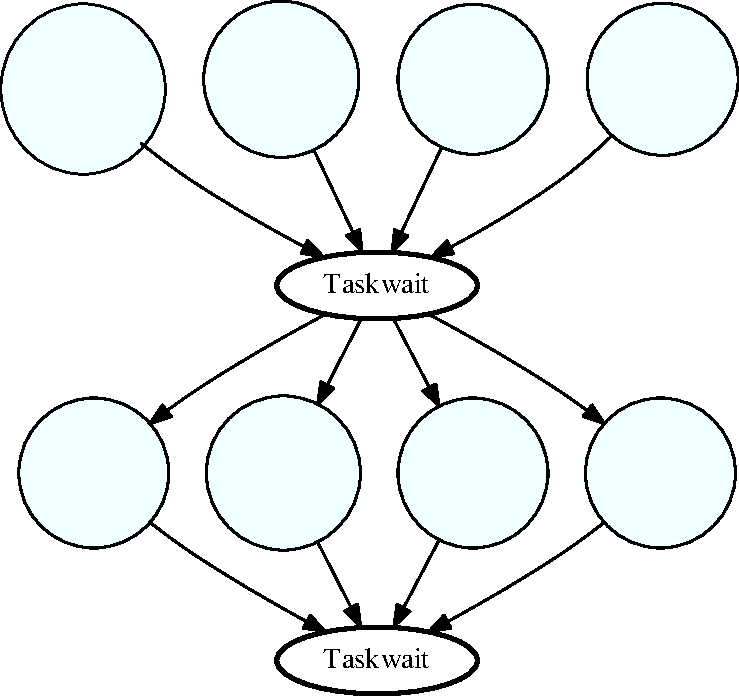
\includegraphics[width=0.5\columnwidth]{ifcg/figures/blackscholes_taskgraph}%
	\caption{Task-graph of blackscholes application.  No dependencies exit between tasks,
only barrier synchronization between iterations.}
	\label{fig:blackscholes_tg}%
	\vspace{.5cm}
\end{figure}

\paragraph{\textit{Pthreads}} This version simply divides the portfolio into
work units by the number of available threads, and stores them into the
\texttt{numOptions} array. Each thread calculates the prices for its
corresponding options and waits in a barrier until all the threads have
finished executing. The algorithm is run multiple times to obtain the final
estimation of the portfolio.


\paragraph{\textit{Task-based}} In the case of the task-based version, we
divide the work into units of a predefined block size. This block size allows
having much more task instances than threads, which implies a much better load
balance, as this is an embarrassingly parallel application with no dependencies
among tasks in the same run.  A task graph of the task-based implementation is
shown in figure \ref{fig:blackscholes_tg}.  We can see that this is an embarrassing
parallel application with only barrier synchronization between iterations of the 
main loop.  No data dependencies exist between tasks.
For all the task graphs shown in this document
we use smaller workloads than the ones used for evaluation.  This way it's easier
to read the task graphs.  For example in figure \ref{fig:blackscholes_tg} there are
four tasks per iteration, but this is easily configurable to hundreds or thousands 
of tasks.  Such is the case of the native workloads used for the evaluation of our 
implementations.



\begin{figure*}[ht!]
	\vspace{1cm}
	\centering
  \begin{subfigure}{0.9\textwidth}
		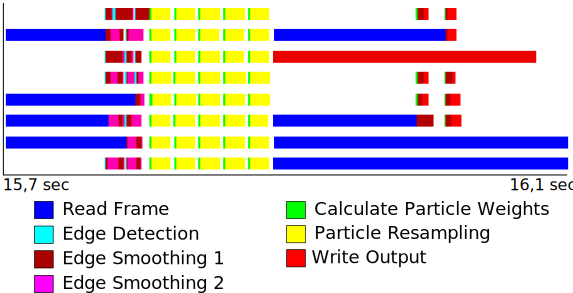
\includegraphics[width=\textwidth]{ifcg/figures/bodytrack-ompss-native-8-2dp_tasks_pthreads}
		\caption{Trivial Task-based Strategy}
	\label{fig:bodytrack-2dp_tasks-trace_pthreads}
  \end{subfigure}%
\\
\vspace{1cm}
\begin{subfigure}{0.9\textwidth}
		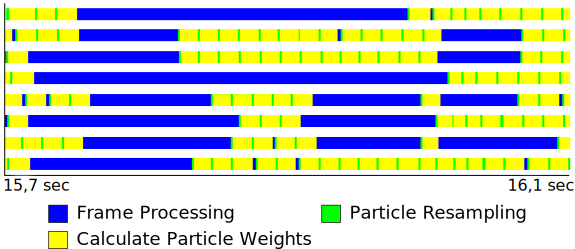
\includegraphics[width=\textwidth]{ifcg/figures/bodytrack-ompss-native-8-2dp_tasks_ompss}
		\caption{Optimal Task-based Strategy}
	\label{fig:bodytrack-2dp_tasks-trace_ompss}
  \end{subfigure}
	\caption{Parallel execution of Pthreads and task-based versions of \texttt{bodytrack} on an 8-core machine and native input size. Different parallel regions correspond to different colors.  White gaps in the figure, represent idle time.}%
	\label{fig:bodytrack-2dp_tasks-trace}%
\end{figure*}

\paragraph{\textbf{Bodytrack}}
Computer vision application that tracks a marker-less human body using multiple cameras
through an image sequence.  The application employs an annealed particle filter to track
the body using edges and the foreground silhouette as features of interest.

\begin{figure}[t!]%
	\center
	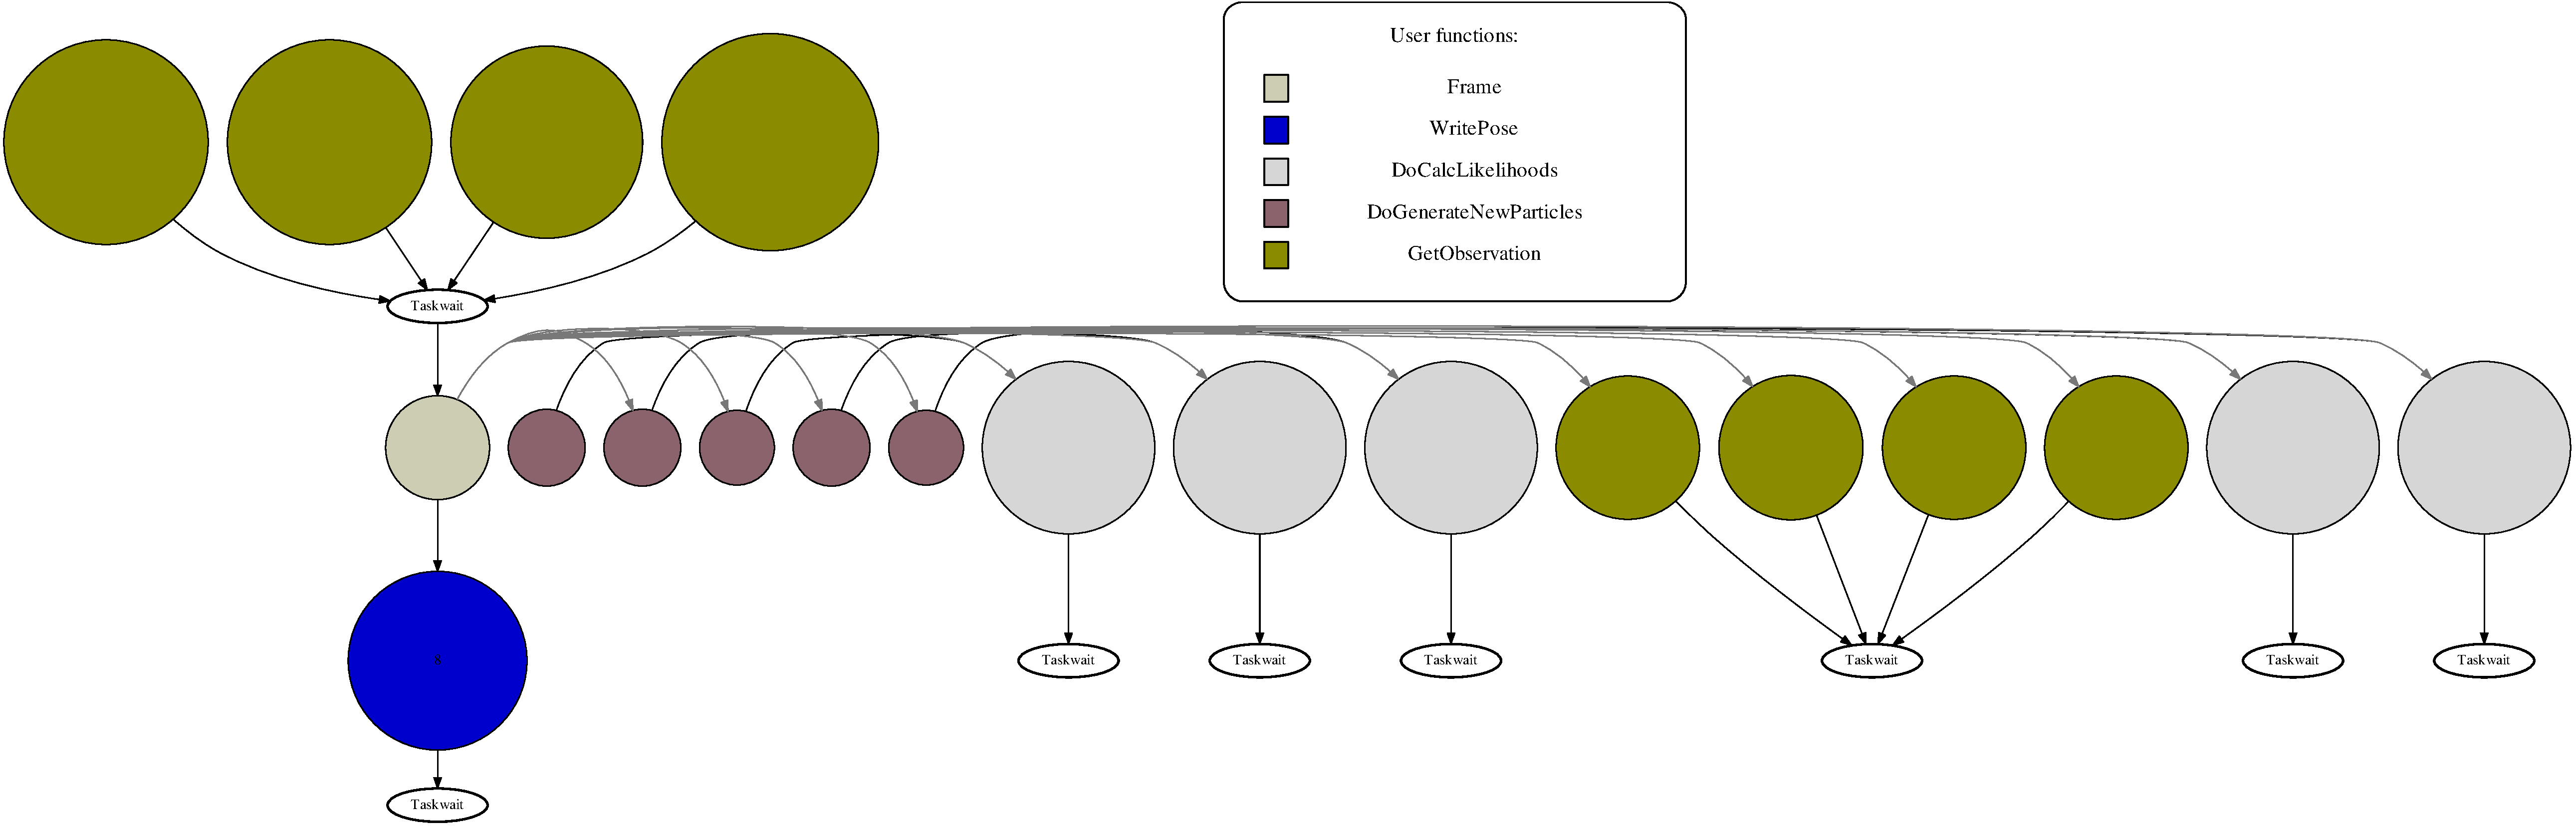
\includegraphics[width=\columnwidth]{ifcg/figures/bodytrack_taskgraph}%
	\caption{Task-graph of bodytrack application.  Edges show task data dependencies.}
	\label{fig:bodytrack_tg}%
	\vspace{.5cm}
\end{figure}



\paragraph{\textit{Pthreads}} \texttt{Bodytrack} applies the same algorithm on each frame
of the image sequence to track the different poses of the body.  The human body is modeled
as a tree-based structure, consisting of 7 conic cylinders.  It reads 4 images taken from
several cameras to capture a scene from 4 different angles, thus each frame consists of
these 4 images.  These images are read and encoded to a single data structure.  For each
frame, \texttt{bodytrack} extracts the edges and silhouette features for each of these 4
images.
In this feature extraction stage we have 3 different kernels.
\begin{enumerate}
	\item \textbf{Edge detection}: Gradient based edge detection.
	\item \textbf{Edge smoothing (phase 1)}: Gaussian filter used to smooth edges applied on array rows.
	\item \textbf{Edge smoothing (phase 2)}: Gaussian filter used to smooth edges applied on array columns.
\end{enumerate}
Afterwards, \texttt{bodytrack} goes through an annealed particle filter stage, which
consists of M annealing layers over a set of N particles.  The particles are multi-variate
configurations of the state and location of the tracked body.  Given the image features,
the particles are assigned weights, which increase or decrease the chance that a particle
represents a body part.  N particles are then chosen, depending on the probability
dictated by their weights.  Random noise is added to this set of particles, creating a new
set.  This process is repeated for all annealing layers. \texttt{Bodytrack} then picks one
of the M configurations, the one which has the highest weighted average.  This process has
two parallel kernels.
\begin{enumerate}[resume]
	\item \textbf{Calculate particle weights}: Computes weights for the particles, using the edges and silhouette produced from the previous stages.
	\item \textbf{Particle Resampling}: Adds Gaussian random noise to the particles, thus creating a new set of particles.
\end{enumerate}

In the case of Pthreads, the 4 images of a frame are read and processed in parallel using
one thread per image.  The Pthreads implantation is limited by the 4 images it can process
concurrently, while there is no other candidate work at this point.  A specific
asynchronous I/O implementation is required to read the files in parallel. Then, the
features extraction stage is executed using all the available threads, with a
synchronization barrier at the end of each phase. The same structure is followed in the
annealed particle filter stage, with two barriers at the end of each phase. Between the
two stages, serial code has to be executed, which leaves only one thread busy and the rest
idle.  Finally, the output results are written sequentially in one file.   


\paragraph{\textit{Task-based}} In the case of the task-based version, we adopt a more coarse grain approach. 
We do not parallelize the feature extraction stage, instead we 
taskify the whole frame processing, allowing concurrent execution of all frames. 
%Given enough frames to process, all threads can remain busy,
%which is not the case with the Pthreads version.
The parallel kernels of the annealed particle filter stage are taskified in our version, and synchronization is achieved
by dataflow annotations.  Figure \ref{fig:bodytrack_tg} shows a task graph of our implementation.  The directed edges show the
dependencies between the different tasks, which dictate the execution order of the tasks.
Each frame needs to be written when calculations are completed. In our version we can do this asynchronously while the threads are
busy with the processing stage of another frame.  Thus, output I/O is effectively overlapped with computation stages.


{Figure \ref{fig:bodytrack-2dp_tasks-trace} shows parallel executions of two different task-based implementations: 
The first one just mimics the Pthreads behavior (\ref{fig:bodytrack-2dp_tasks-trace_pthreads}) and the second is an optimal task-based implementation (\ref{fig:bodytrack-2dp_tasks-trace_ompss}).  
Different colored boxes represent different task types, as well the duration of that task type on each core. In both cases, the white gaps denote the time each thread spends idle.  
Both figures show the same duration for each execution. In the optimal version, all functionality is implemented within the frame-processing task, thus 
execution time for read-frame, edge-detection and edge-smoothing is represented with blue color (frame-processing).  
Tasks particle-resampling and calculate-particle-weights are also implemented as nested tasks. 
They are displayed with different colors (green and yellow respectively).  
We can observe that the Pthreads-like version suffers
from greater idle time compared to its optimal task-based counterpart. 
Work is distributed more efficiently in the optimal implementation
by processing different frames concurrently. 
This allows us to overlap I/O and serial code segments of one with available work from another one.
       
%To illustrate this point, Figure~\ref{fig:bodytrack-2dp_tasks-trace} shows an execution of \texttt{bodytrack} for two different frames. The x-axis represent time and the y-axis represent the cores where the execution takes place. 
%For example, a pixel of color blue in the (x,y) point means that at the instant x the core y is running the task codified by color blue. The red, dark red and green are tasks performing edge detection and edge smoothing, respectively.  
%The yellow color represents the task writing the output file. 
%Light green and magenta are the tasks that calculate particle weights and re-sample the particles. Light blue color annotates the idle time or sequential code execution. 
%%
%We can see how the task that writes the output file for frame N-1 (in yellow) is overlapped by the three first computation tasks of frame N, which does not happen in the Pthreads version of the code.
%This overlapping is the main source of performance gains archived by using the dataflow task-based paradigm with \texttt{bodytrack}. 
%Section~\ref{sec:evaluation} reports these improvements in detail.

\paragraph{\textbf{Canneal}}
This kernel uses a cache-aware simulated annealing~\cite{Banerjee:1994:PAV:185340} to
optimize routing cost of a chip design.  \texttt{Canneal} progressively swaps elements
that need to be placed in a large space, eventually converging to an optimal solution. The
problem is stored as a list with routing costs between nodes. 

\begin{figure}[t!]%
	\center
	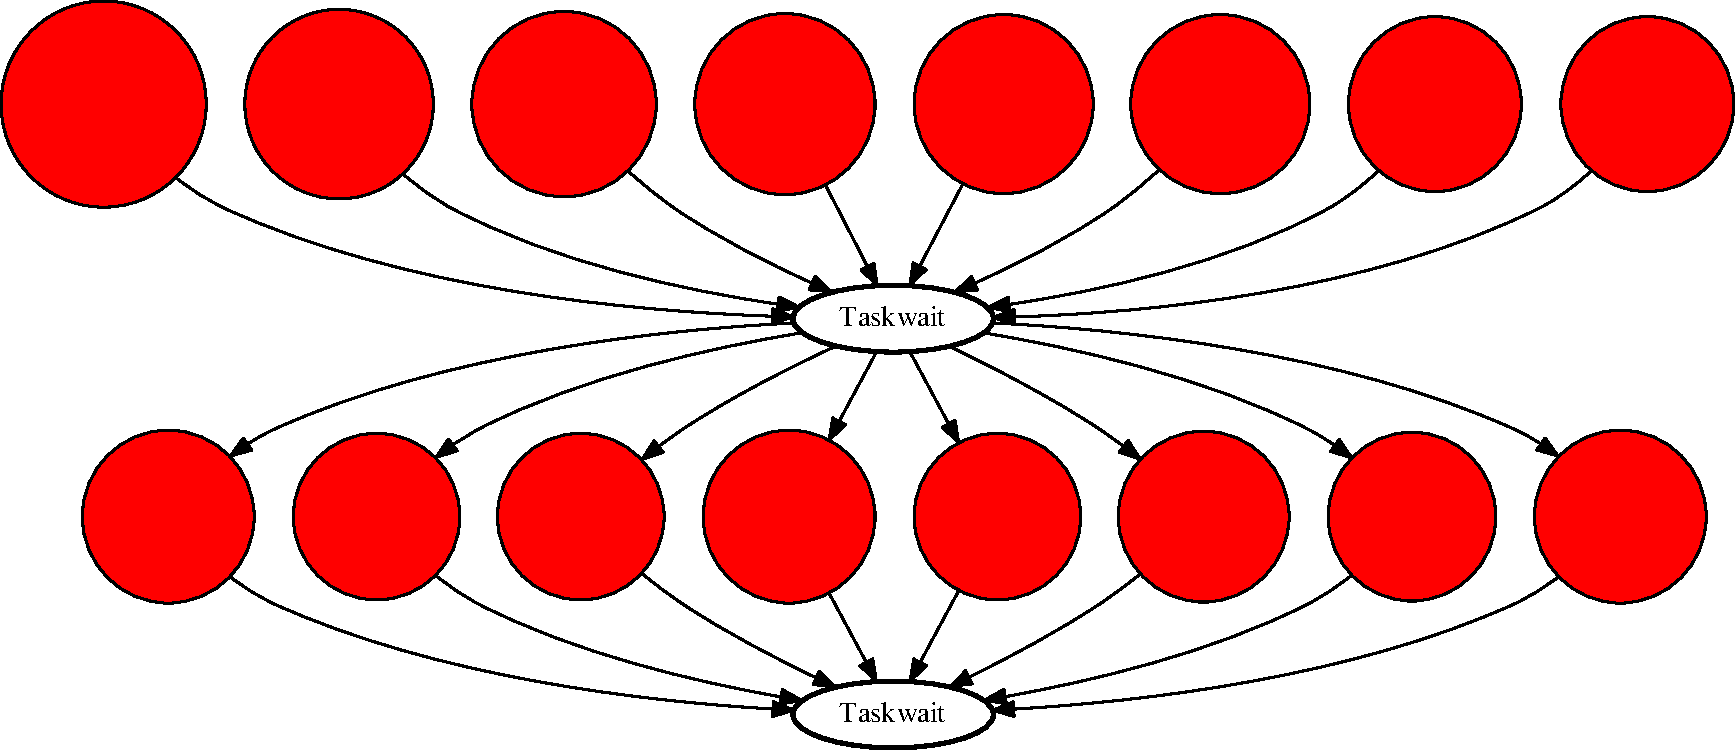
\includegraphics[width=.8\columnwidth]{ifcg/figures/canneal_taskgraph}%
	\caption{Task-graph of canneal application.  Only barrier synchronization among tasks.}
	\label{fig:canneal_tg}%
	\vspace{.5cm}
\end{figure}

\paragraph{\textit{Pthreads}} This version compares random element pairs of the graph
concurrently and swaps them until it converges to an optimal solution.  No locks are used
to protect the list from concurrent accesses/writes, but  swaps are done atomically
instead. However, the evaluation of the elements to be swapped is not atomic.  This means
that disadvantageous swaps may occur, which will require the algorithm to eventually swap
them again.  This method has provided better results than the alternative algorithm with
locks~\cite{bienia2008}.

\paragraph{\textit{Task-based}} Our task-based version follows the same paradigm.  Several
tasks are spawned without any dependencies between themselves. We use the same atomics as
with the Pthreads version.  Since tasks work with an arbitrary number of list elements, it
is not possible to describe which elements of the list a task is going to randomly access. 
In the task graph in figure \ref{fig:canneal_tg} it is clear that there are no data dependencies.
Synchronization is only achieved through the use of barriers.

We also try an alternative fine grain implementation, where a task is spawned for each
random pair of list elements.  This would allow the runtime to know if two tasks are
working on the same list of elements. However this implementation implied fine-grain
tasks. Each task would merely do a single swap between two list elements.  The overhead of
the dynamic scheduling is a problem in this scenario.  A more complex but more efficient
solution is suggested by Symeonidou et al.~\cite{Symeonidou:2013:DDR:2488551.2488558} with
the use of memory regions.  Adopting this method in a task-based model would allow the
programmer to describe parts of the list (or other pointer based data structures) and
express dataflow relations as abstract memory regions.  This solution also implies
fine-grain tasking and is not evaluated at the Symeonidou's work. 

\begin{figure}[t!]%
	\center
	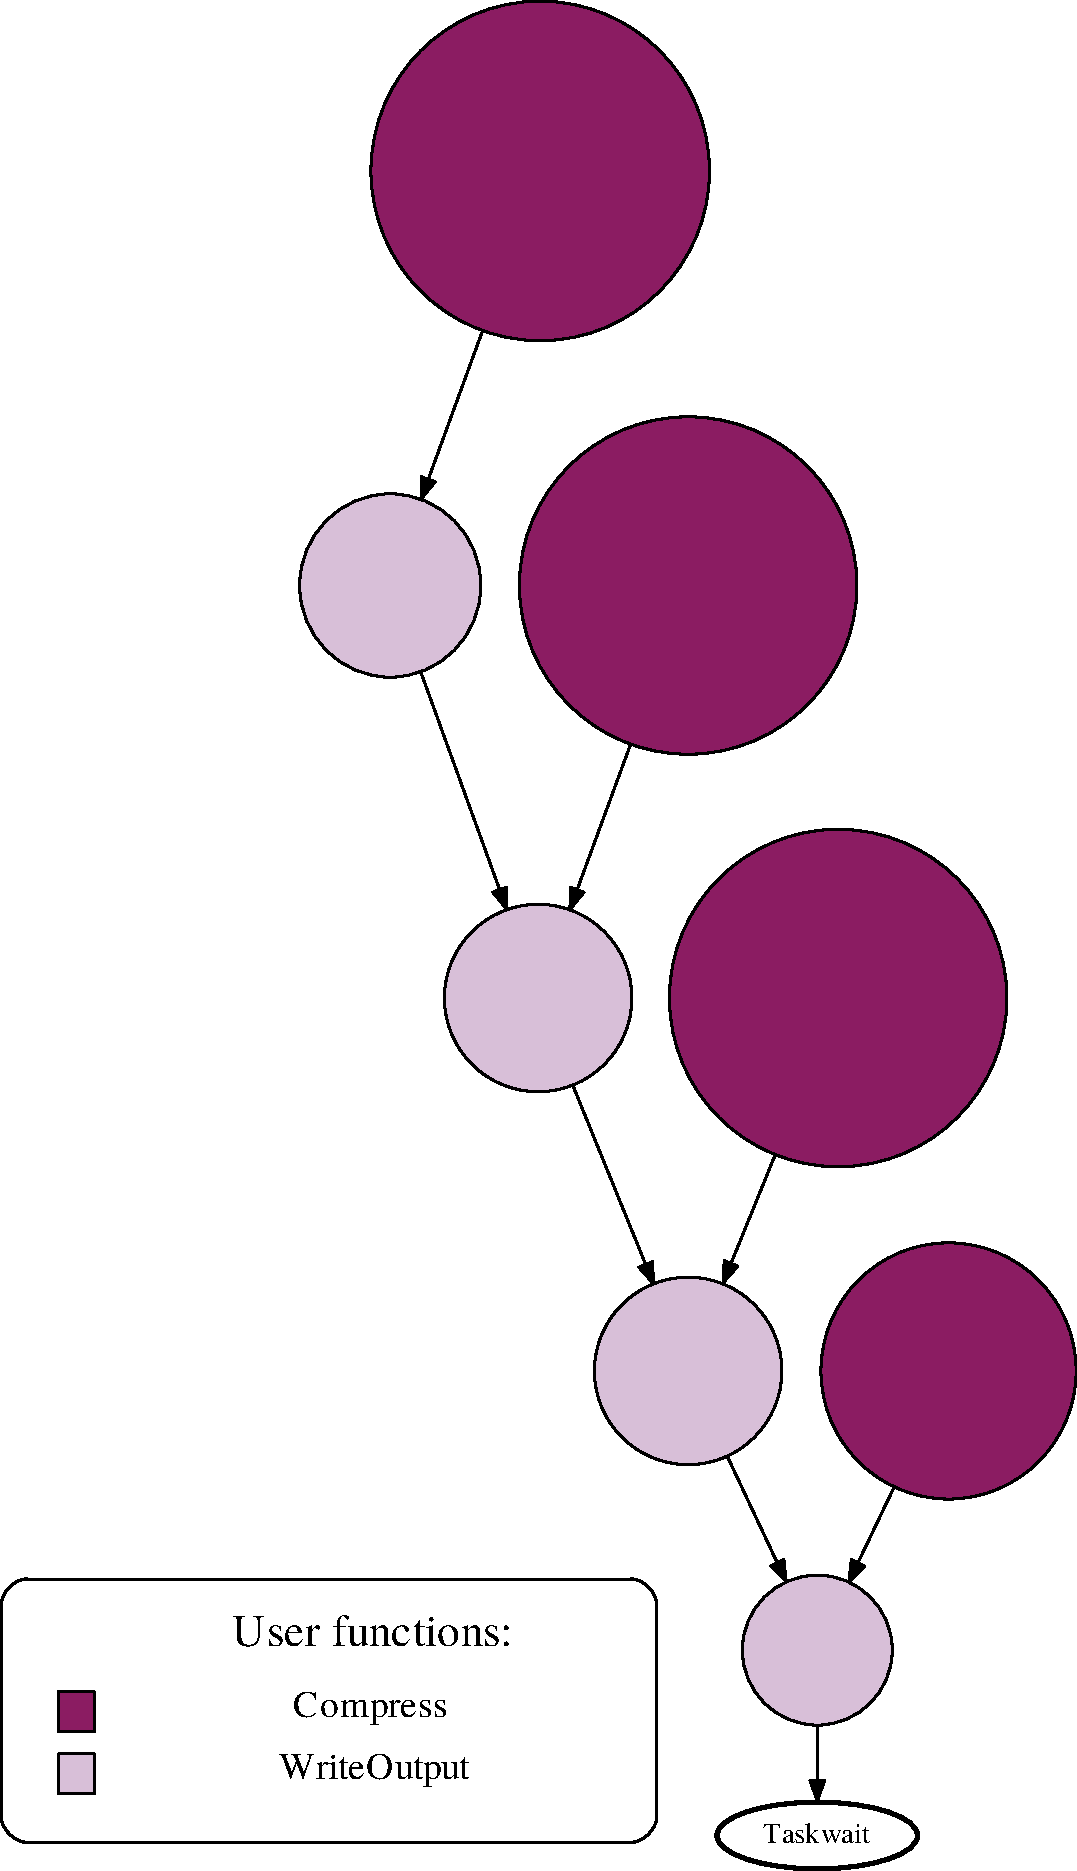
\includegraphics[width=.4\columnwidth]{ifcg/figures/dedup_taskgraph}%
	\caption{Task-graph of dedup application.  Data dependency edges force the correct order
of writting the data chunks to the output.}
	\label{fig:dedup_tg}%
	\vspace{.5cm}
\end{figure}


\paragraph{\textbf{Dedup}}
The \texttt{dedup} kernel is used to compress data streams using local and global
compression to achieve higher compression rates.  This method is called
deduplication~\cite{Quinlan:2002:ABP:1083323.1083333}.

\paragraph{\textit{Pthreads:}}
Dedup is parallelized using a pipeline model with the following stages:
\begin{itemize}
  \item \textbf{Fragment}:  First, the data-stream is read and partitioned at fixed positions into coarse grain data chunks. Each chunk can be processed individually by the rest of the stages. This stage is executed on a single thread.
  \item \textbf{Fragment Refine}:  A new data chunk initiates the second pipeline stage, where it is further partitioned into smaller fine-grain
	chunks.  The portioning is done by using the Rolling-fingerprint algorithm.  
  \item \textbf{Deduplication}:  This stage eliminates duplicate fine-grain chunks.  Unique chunks are stored in a hash-table.
	Locks are used here to protect	each bucket from concurrent accesses.
  \item \textbf{Compress}:  At this stage chunks are compressed in parallel.  Identical chunks are compressed only once as duplicates are removed 
	at the deduplication stage.
  \item \textbf{Reorder}:  This stage writes the final compressed output data to a file.  It writes only unique chunks' compressed data and for the
	duplicates it stores their hash values.  However this stage needs to reorder the data chunks as they are received
	to match the original order of the uncompressed data.
\end{itemize}

The Pthreads version maintains a queue and a thread pool dedicated to each stage.  When a
chunk becomes available at one stage, it is moved to the queue of the next stage.  Each
stage polls at its queue for available chunks to process. The reorder stage is done
sequentially with a devoted thread that can be in an idle loop waiting for previous stages
to finish.  Each thread pool  comprises by a number of threads equal to the number of
available cores.  The only exceptions are \texttt{Fragment} and \texttt{Reorder} stages,
which are served by a single thread each.

%\begin{figure}[ht!]%
%	\centering
%	\begin{lstlisting}
%void Fragment{
%  ...
%  while ( chunk = read_bytes() ) {
%		chunks[nCChunks][0] = chunk;
%		#pragma omp task inout(chunks[nCChunks]) 
%		Fragment(chunks[nCChunks]);
%		#pragma omp task inout(chunks[nCChunks])
%		WriteOutput(outfile, chunks[nCChunks]);
%		nCChunks++;
%		break;
%  }
%  #pragma omp taskwait
%	...
%}
%	\end{lstlisting}
%	\caption{Dedup task-based implementation pseudocode of the \texttt{Fragment} stage.}%
%	\label{lst:dedup-ompss}%
%\end{figure}

\begin{figure}[!t]%
	\centering
	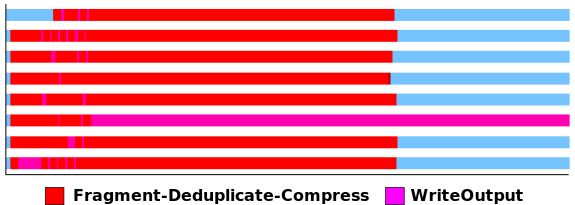
\includegraphics[width=0.9\columnwidth]{ifcg/figures/dedup-ompss-native-8-2dp_tasks}%
	\caption{Parallel execution of the task-based version of \texttt{dedup} on an 8-core machine and native input size. Different task types correspond to different colors.}%
	\label{fig:dedup-2dp_tasks-trace}%
	\vspace{.5cm}
\end{figure}


\paragraph{\textit{Task-based}}
In our implementation we taskify each pipeline stage and express data dependencies using static arrays and dataflow relations, one for each pipeline stage.
\texttt{FragmentRefine} however partitions the data chunks into very fine grain segments, ranging from a few hundreds to thousands. For such granularity,
our approach suffers from high overheads due to dynamic schedulnig overhead. 
The same is observed in~\cite{Vandierendonck:2013:DSP:2503210.2503233}, where 
an alternative approach is adopted. In their approach, two pipelines are identified: The outer pipeline, consisting of stages \texttt{Fragment}, \texttt{InnerPipeline}
and \texttt{Reorder}. The inner pipeline consists of \texttt{FragmentRefine}, \texttt{Deduplicate} and \texttt{Compress}.  To reduce the dynamic scheduling overhead,
they merge together \texttt{Deduplicate} and \texttt{Compress}. By doing so, the available parallelism is limited, but still there is enough work not to harm performance
and scalability. In our approach, we merge together the inner pipeline, creating one sequential function, exploiting only the parallelism available in the outer pipeline.
Even in this scenario, the available parallelism is still abundant, since the application is bound by the writing of the output file, which is sequential.  
Figure~\ref{fig:dedup-2dp_tasks-trace} shows a trace of the task-based version.  We can see that communication stage (in yellow) is effectively overlapped with the computation stage (in red), however,
there is not enough work to keep all the threads finish, until the end of the execution.

Furthermore, we modify the \texttt{Reorder} stage, by replacing it with a simple stage where the chunk is simply written to file (\texttt{WriteOutput}).
Using dataflow relations and a shared output resource between the \texttt{WriteOutput} tasks, we ensure that chunk \texttt{N-1} will be written before chunk \texttt{N}. 
Thus, we do not need to reorder data chunks in this task type.  Moreover, the scheduler makes sure chunks are written as soon as they become available by the \texttt{InnerPipeline} task, an improvement
over the Pthreads version, where \texttt{Reorder} instances need to idle wait until all previous chunks ones have been written.  
Figure \ref{fig:dedup_tg} shows the dependencies among tasks.  We can observe that \texttt{WriteOutput} tasks will be run in the correct
order, as soon as their dependencies are resolved.
Another difference between the two versions, is that Pthreads 
oversubscribe threads to cores for each pipeline stage, while in our implementation we only assign one thread to each core.


\paragraph{\textbf{Facesim}}
Computes a visually realistic human face animation by simulating the underlying physics.  As input it uses a 3D model of a human face 
containing both a tetrahedra mesh and triangulated surfaces for the flesh and bones, respectively. Additionally it uses 
a time sequence of muscle movement \cite{Sifakis:2005:ADF:1073204.1073208}.

\paragraph{\textit{Pthreads}}
The application statically decomposes the original tetrahedron mesh into smaller partitions, equal to the number of available threads.
%The boundaries of the partitions are replicated to avoid synchronization. The trade-off is redundant computations. For the bones, they 
%are employed serially. 
There are three main parallel kernels:
\begin{itemize}
  \item \textbf{Update State}: Calculates the steady properties of the mesh, constrains like stress and stiffness.  
%This is done by solving a nonlinear system of equationsusing the Newton-Rhapson method.  
  \item \textbf{Add Forces}: Computes the force contribution between vertices acting on the 3D model.
  \item \textbf{Conjugate Gradient (CG)}:  An iterative method that solves the linear system produced by the 
other two previous kernels and find the final displacement of the vertices for the current frame.
\end{itemize}

\texttt{Update\_State} and \texttt{Add\_Forces} kernels consist of one and two parallel loops respectively, while \texttt{CG} has three. 
Synchronization between loops and kernels is achieved by barriers.  The corresponding force computations from the skeleton are also done 
in \texttt{Update\_State} and \texttt{Add\_Forces}, but after the parallel computations on the tetrahedra mesh have been made. 
In Pthreads a master thread is assigning work to all threads in a round-robin fashion through a queuing system.  Each thread maintains 
its private queue, which is protected by locks.

%\begin{figure}[!t]%
%	\centering
%	\includegraphics[width=0.8\columnwidth]{figures/facesim-ompss-native-8-2dp_tasks}%
%	\caption{Parallel execution of the task-based version of \texttt{facesim} on an 8-core machine while simulating a frame. 
%	Different task types correspond to different colors, while idle time is represented in light blue color.}%
%	\label{fig:facesim-2dp_tasks-trace}%
%\end{figure}

\paragraph{\textit{Task-based}}
In the task-based version, the application level queuing system is completely replaced by the OmpSs runtime.  In our initial implementation 
all parallel loops are taskified. 
Additionally,  in \texttt{Update\_State} there is a sequential code segment, 
\texttt{Update\_Collision\_Penalty\_Forces}.  
This code segment operates on the bones, while the parallel loop of \texttt{Update State} does so on the tetrahedra.  
By taskifying it and adding dataflow relations between this Section and the following \texttt{Add\_Forces} kernel, we can overlap 
\texttt{Update\_Collision\_Penalty\_Forces} with the rest of \texttt{Update\_State}.


%\edit{In the \texttt{CG} kernel, we managed to remove two out of three barriers, which synchronized the different parallel loops, by using dataflow relations 
%to describe data dependencies.  One barrier could not be removed as it protects the residual calculation at theend of each iteration of the solver, 
%whose value is used to control whether we exit the loop or not.}  
%\edit{This initial implementation suffered from high task creation time in the \texttt{CG} kernel.  Note that this is an issue of OmpSs' runtime, out OpenMP 4.0 task implementation 
%did not manifest this issue.}
To improve performance we refactor tasks' creation in \texttt{CG} by nesting the first task creation loop inside another task.
This enables us to overlap task creation time with computation, which contributes to increase \texttt{Facesim's} task-based implementation performance.  
Although we achieve better scalability than the original code, task creation still imposed overheads. To address this issue
we replace tasks in \texttt{CG} with the OmpSs parallel loops construct (equivalent to the OpenMP one), which implements loop worksharing 
with a task. Even though this approach limits the available parallelism (barrier synchronization, no dataflow annotations), the overhead 
associated to task creation and scheduling is greatly reduced and overall performance improved.

\paragraph{\textbf{Ferret}}
Content similarity search server for feature-rich data~\cite{Lv:2006:FTC:1218063.1217966} like audio, video, images, etc.
The benchmark application is configured for image similarity search.  
%\begin{figure}[t!]%
%	\begin{lstlisting}
%void load() {
%	int i = 0;
%	while( load_image(image[i]) ) {
%		#pragma omp task in(image[i]) out(seg_images[i])
%		seg_images[i] = t_seg(image[i]);
%		#pragma omp task in(seg_images[i]) out(extract_data[i])
%		extract_data[i] = t_extract(seg_images[i]);
%		#pragma omp task in(extract_data[i]) out(vectoriz_data[i])
%		vectoriz_data[i] = t_vec(extract_data[i]);
%		#pragma omp task in(vectoriz_data[i]) out(rank_results[i])
%		rank_results[i] = t_rank(vectoriz_data[i]);
%		#pragma omp task in(rank_data[i]) out(outstream)
%		t_out(rank_data[i], outstream);
%		i++;
%	}
%	#pragma omp taskwait
%}
%	\end{lstlisting}
%	\caption{Ferret ompss implementation}%
%	\label{lst:ferret-ompss}%
%\end{figure}

\begin{figure}[t!]%
	\center
	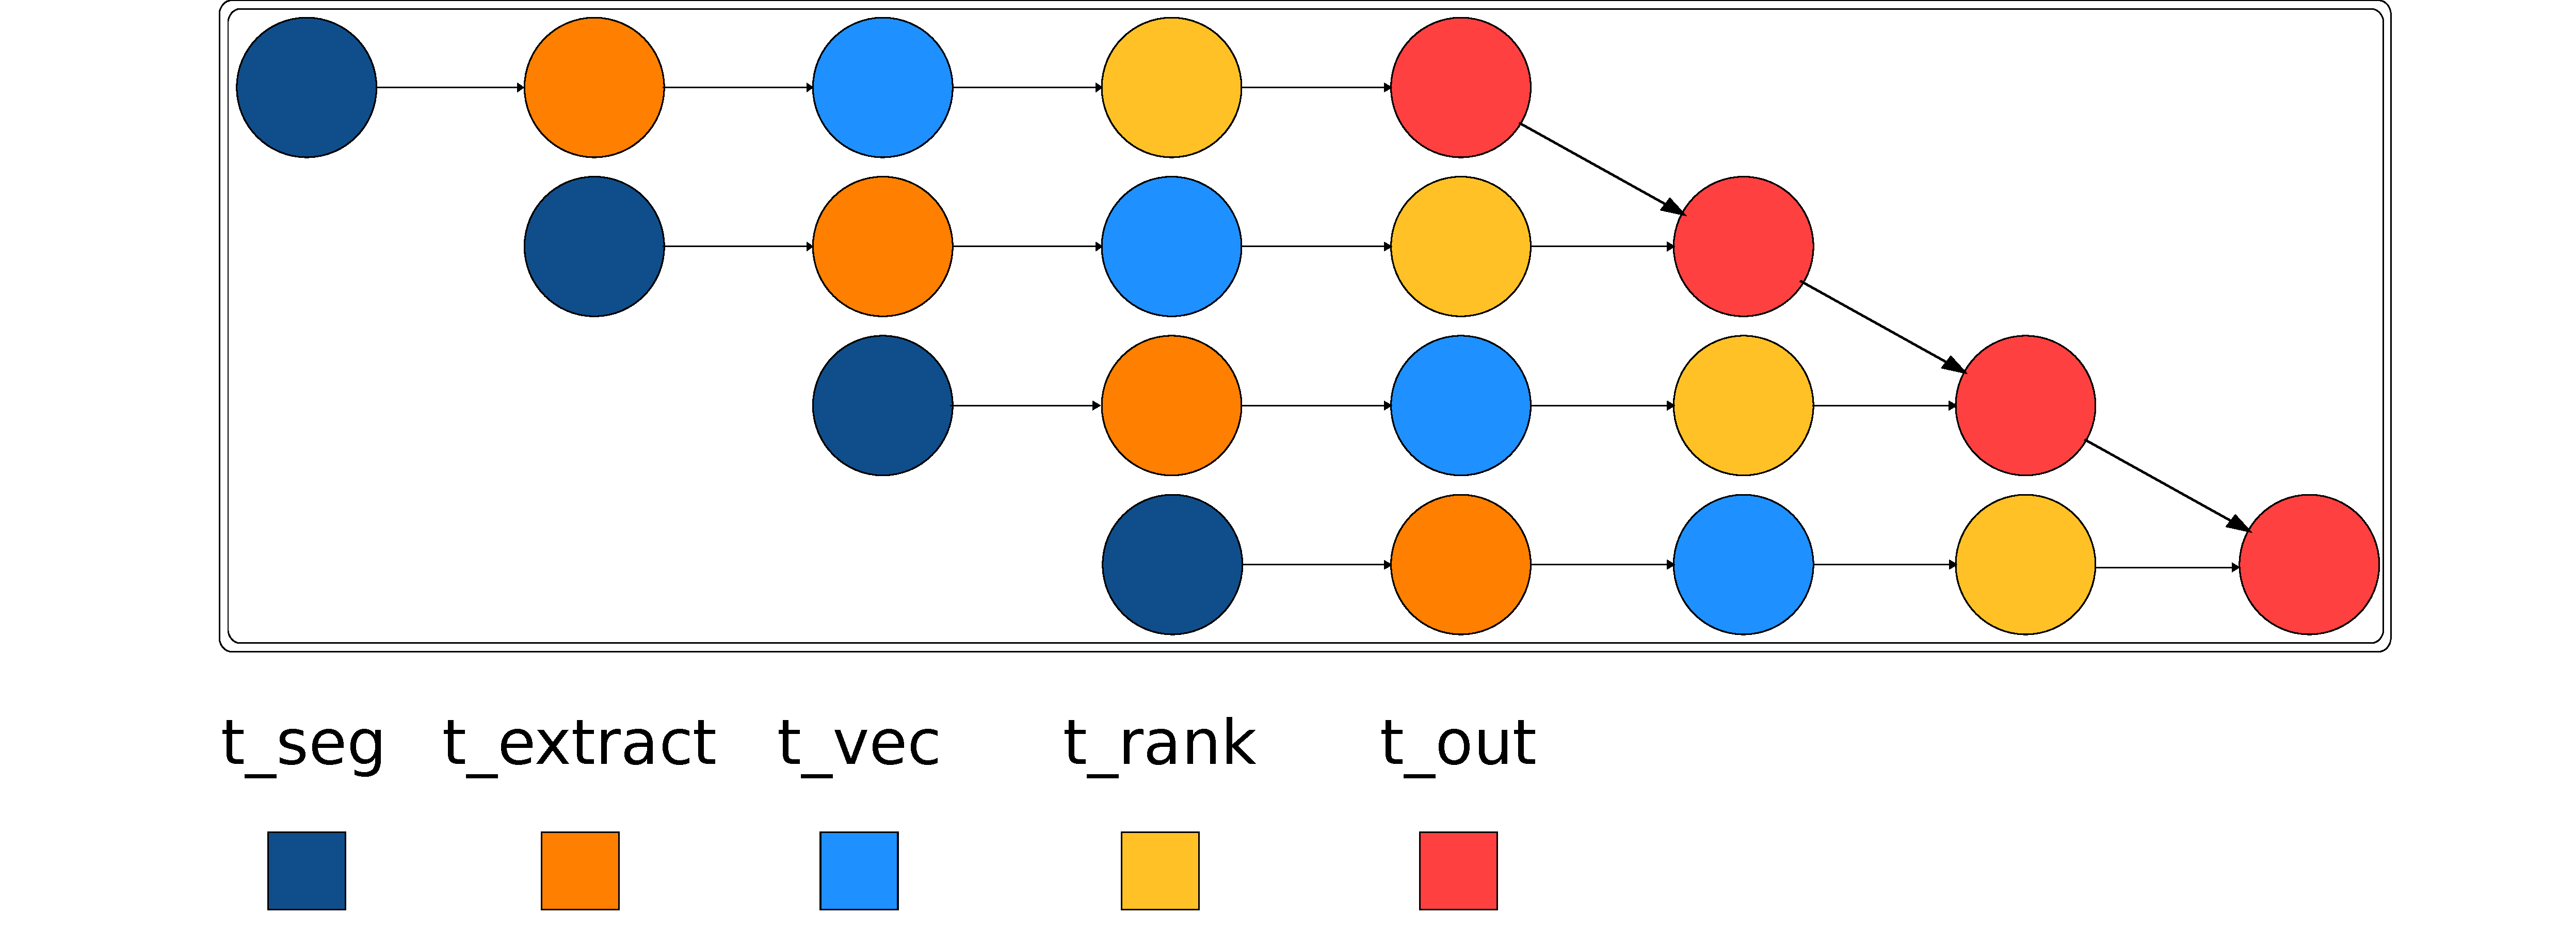
\includegraphics[width=0.9\columnwidth]{ifcg/figures/ferret_tg}%
	\caption{Task-graph of ferret showing the pipelined execution model.  Edges show data dependencies among different tasks.}
	\label{fig:ferret_tg}%
	\vspace{.5cm}
\end{figure}

\paragraph{\textit{Pthreads}}
Ferret is parallelized using a pipeline model.  A serial query is broken down into 
6 pipeline stages:
\begin{itemize}
  \item \textbf{Load}:  This stage loads an image that is going to be used as a query.
  \item \textbf{Segmentation}:  At this stage the image is decomposed into the different objects displayed on it.
	Different weight vectors are to be assigned on each object to achieve better results.
%	For example if an object is identified as a background it will have a smaller weight
%	than other objects.
  \item \textbf{Extract}:  At this stage a 14-dimensional vector is computed for each object from the segmentation stage, 
														describing features such as color, area, state, etc.
  \item \textbf{Vectorization}:  This is the indexing stage that tries to find a set of candidate images in the database.
  \item \textbf{Rank}:  This stage ranks the results found, using the EMD metric for each query-object's vector
	and the database's image vectors.
  \item \textbf{Output}:  Outputs the result of the ranking stage.  Multiple instances of
	this stage need to run serially, since they all share the same output stream.

\end{itemize}

In the Pthreads version every stage is served by a dedicated thread-pool of N threads each, where N is the number of available cores.
The only exceptions are the \texttt{Load} and \texttt{Output} stages that are executed by a respective single thread.
Each stage polls on its corresponding queue for available work.  When a stage finishes,
it pushes the results to the next stage's queue. 

\paragraph{\textit{Task-based}}
In this version, we implement a variation of this pipeline model. As soon as the first
stage, \texttt{Load}, finds a new image, it spawns all stages of a pipeline for that
image, thus reducing the pipeline to five stages.  We model the dataflow relations between
different stages as simple one dimension arrays, as shown in
Figure~\ref{lst:ferret-ompss}.  Tasks working on different image queries do not share any
dependencies. An exception is task \texttt{t\_out} which shares the same output file
between all pipelines, thus sequential execution is forced between all instances of this
task.  The pipeline stages and dependencies are constructed a priori, which is good enough
for this application, but this is not always the case.
\cite{Lee:2013:OPP:2486159.2486174} proposes a system that can handle dynamic pipeline
creation by constructing a DAG with the stages using indexes and the
\texttt{cilk\_continue} and \texttt{cilk\_wait} keywords.  Indexes are used to define the
different pipeline stages, while \texttt{cilk\_continue} creates a stage that can run once
all previous stages in the same pipeline iteration are done, and \texttt{cilk\_wait}
creates a stage that will wait for its stage counterpart of the previous iteration to
finish.  A strategy based on versioning the dependency objects between the stages has been
proposed~\cite{Vandierendonck:2011:PPG:2001252.2001265}.  Output dependencies are renamed
and privatized, thus the static array for privatization is not required.  

Figure \ref{fig:ferret_tg} shows the task-graph of the \texttt{ferret} application.
Colored nodes denote the concurrent tasks (each color matches a specific task type).
Tasks that have data dependencies are connected by directed edges.  By inspecting the
task-graph we can see a pipeline pattern of execution.  Despite the fact that the
task-based approach does not significantly improve the overall performance, as we can see
in Section~\ref{sec:task_bench_evaluation}, it significantly reduces the effort required
to express the pipeline parallelism, compared its Pthreads counterpart, as it is shown in
Section~\ref{sec:lines} in detail.


\paragraph{\textbf{Fluidanimate}}
This application simulates incompressible fluid interactive animation, using the 
Smoothed Particle Hydrodynamics (SPH) method~\cite{Muller:2003:PFS:846276.846298}.

\begin{figure}[t!]%
	\center
	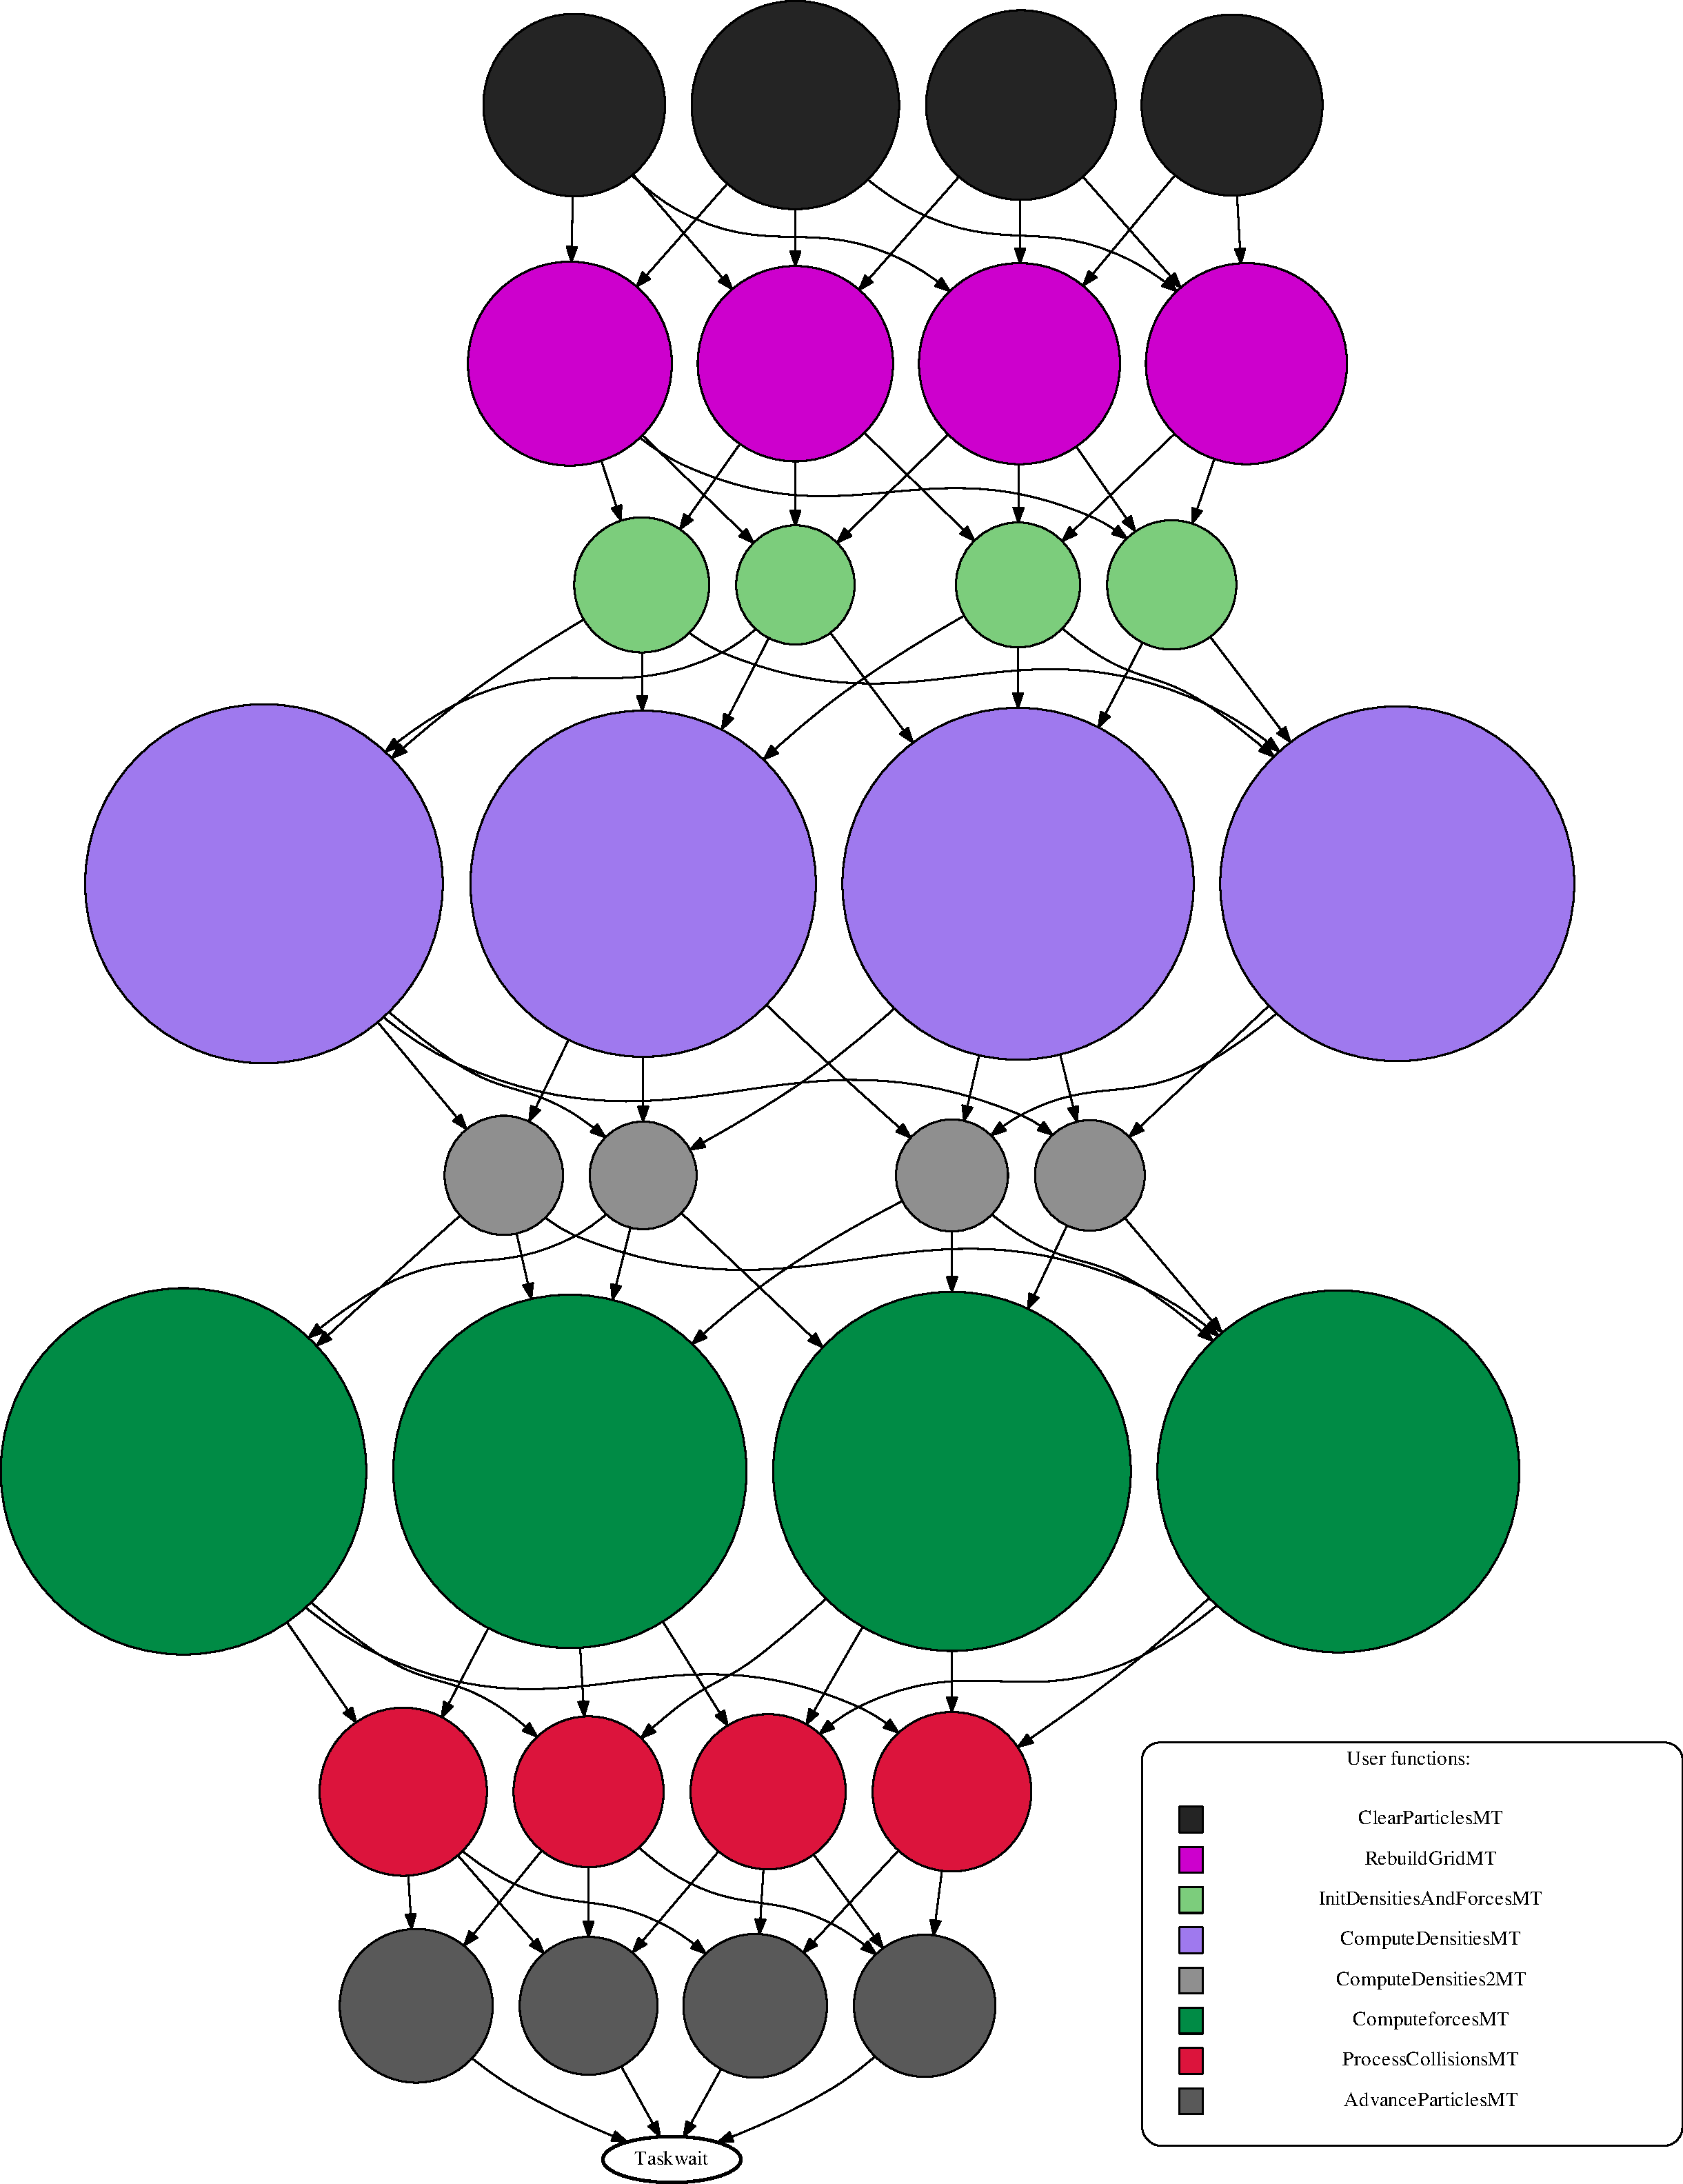
\includegraphics[width=.6\columnwidth]{ifcg/figures/fluidanimate_taskgraph}%
	\caption{Task-graph of fluidanimate application. Edges represent data dependencies among
tasks}
	\label{fig:fluidanimate_tg}%
	\vspace{.5cm}
\end{figure}

\paragraph{\textit{Pthreads}}
\texttt{Fluidanimate} uses five special kernels which are responsible for rebuilding the
spatial index, computing fluid densities and forces at given points, handling fluid
collisions with the scene geometry and finally updating particle locations The fluid
surface is partitioned and each thread works on its own grid segment.  The kernels are
parallelized as do-all loops, separated by barriers. Moreover, there are cases where these
threads need to update values beyond their partition, which are handled using locks.

\paragraph{\textit{Task-based}}
The task-based implementation follows the same approach, we apply a loop tiling
transformation, for each parallel loop, and taskified each iteration.  
Figure \ref{fig:fluidanimate_tg} show how dependencies form among between tasks.  
Tasks from different loops can run concurrently, as soon as their dependencies are met.
For example we see that the first task of each loop, only requires that the first two tasks
from the previous loop finish their execution to have their dependencies resolved.
We maintain the
same barrier and lock synchronization scheme, using the OmpSs synchronization primitives.

\begin{figure}[t!]%
	\center
	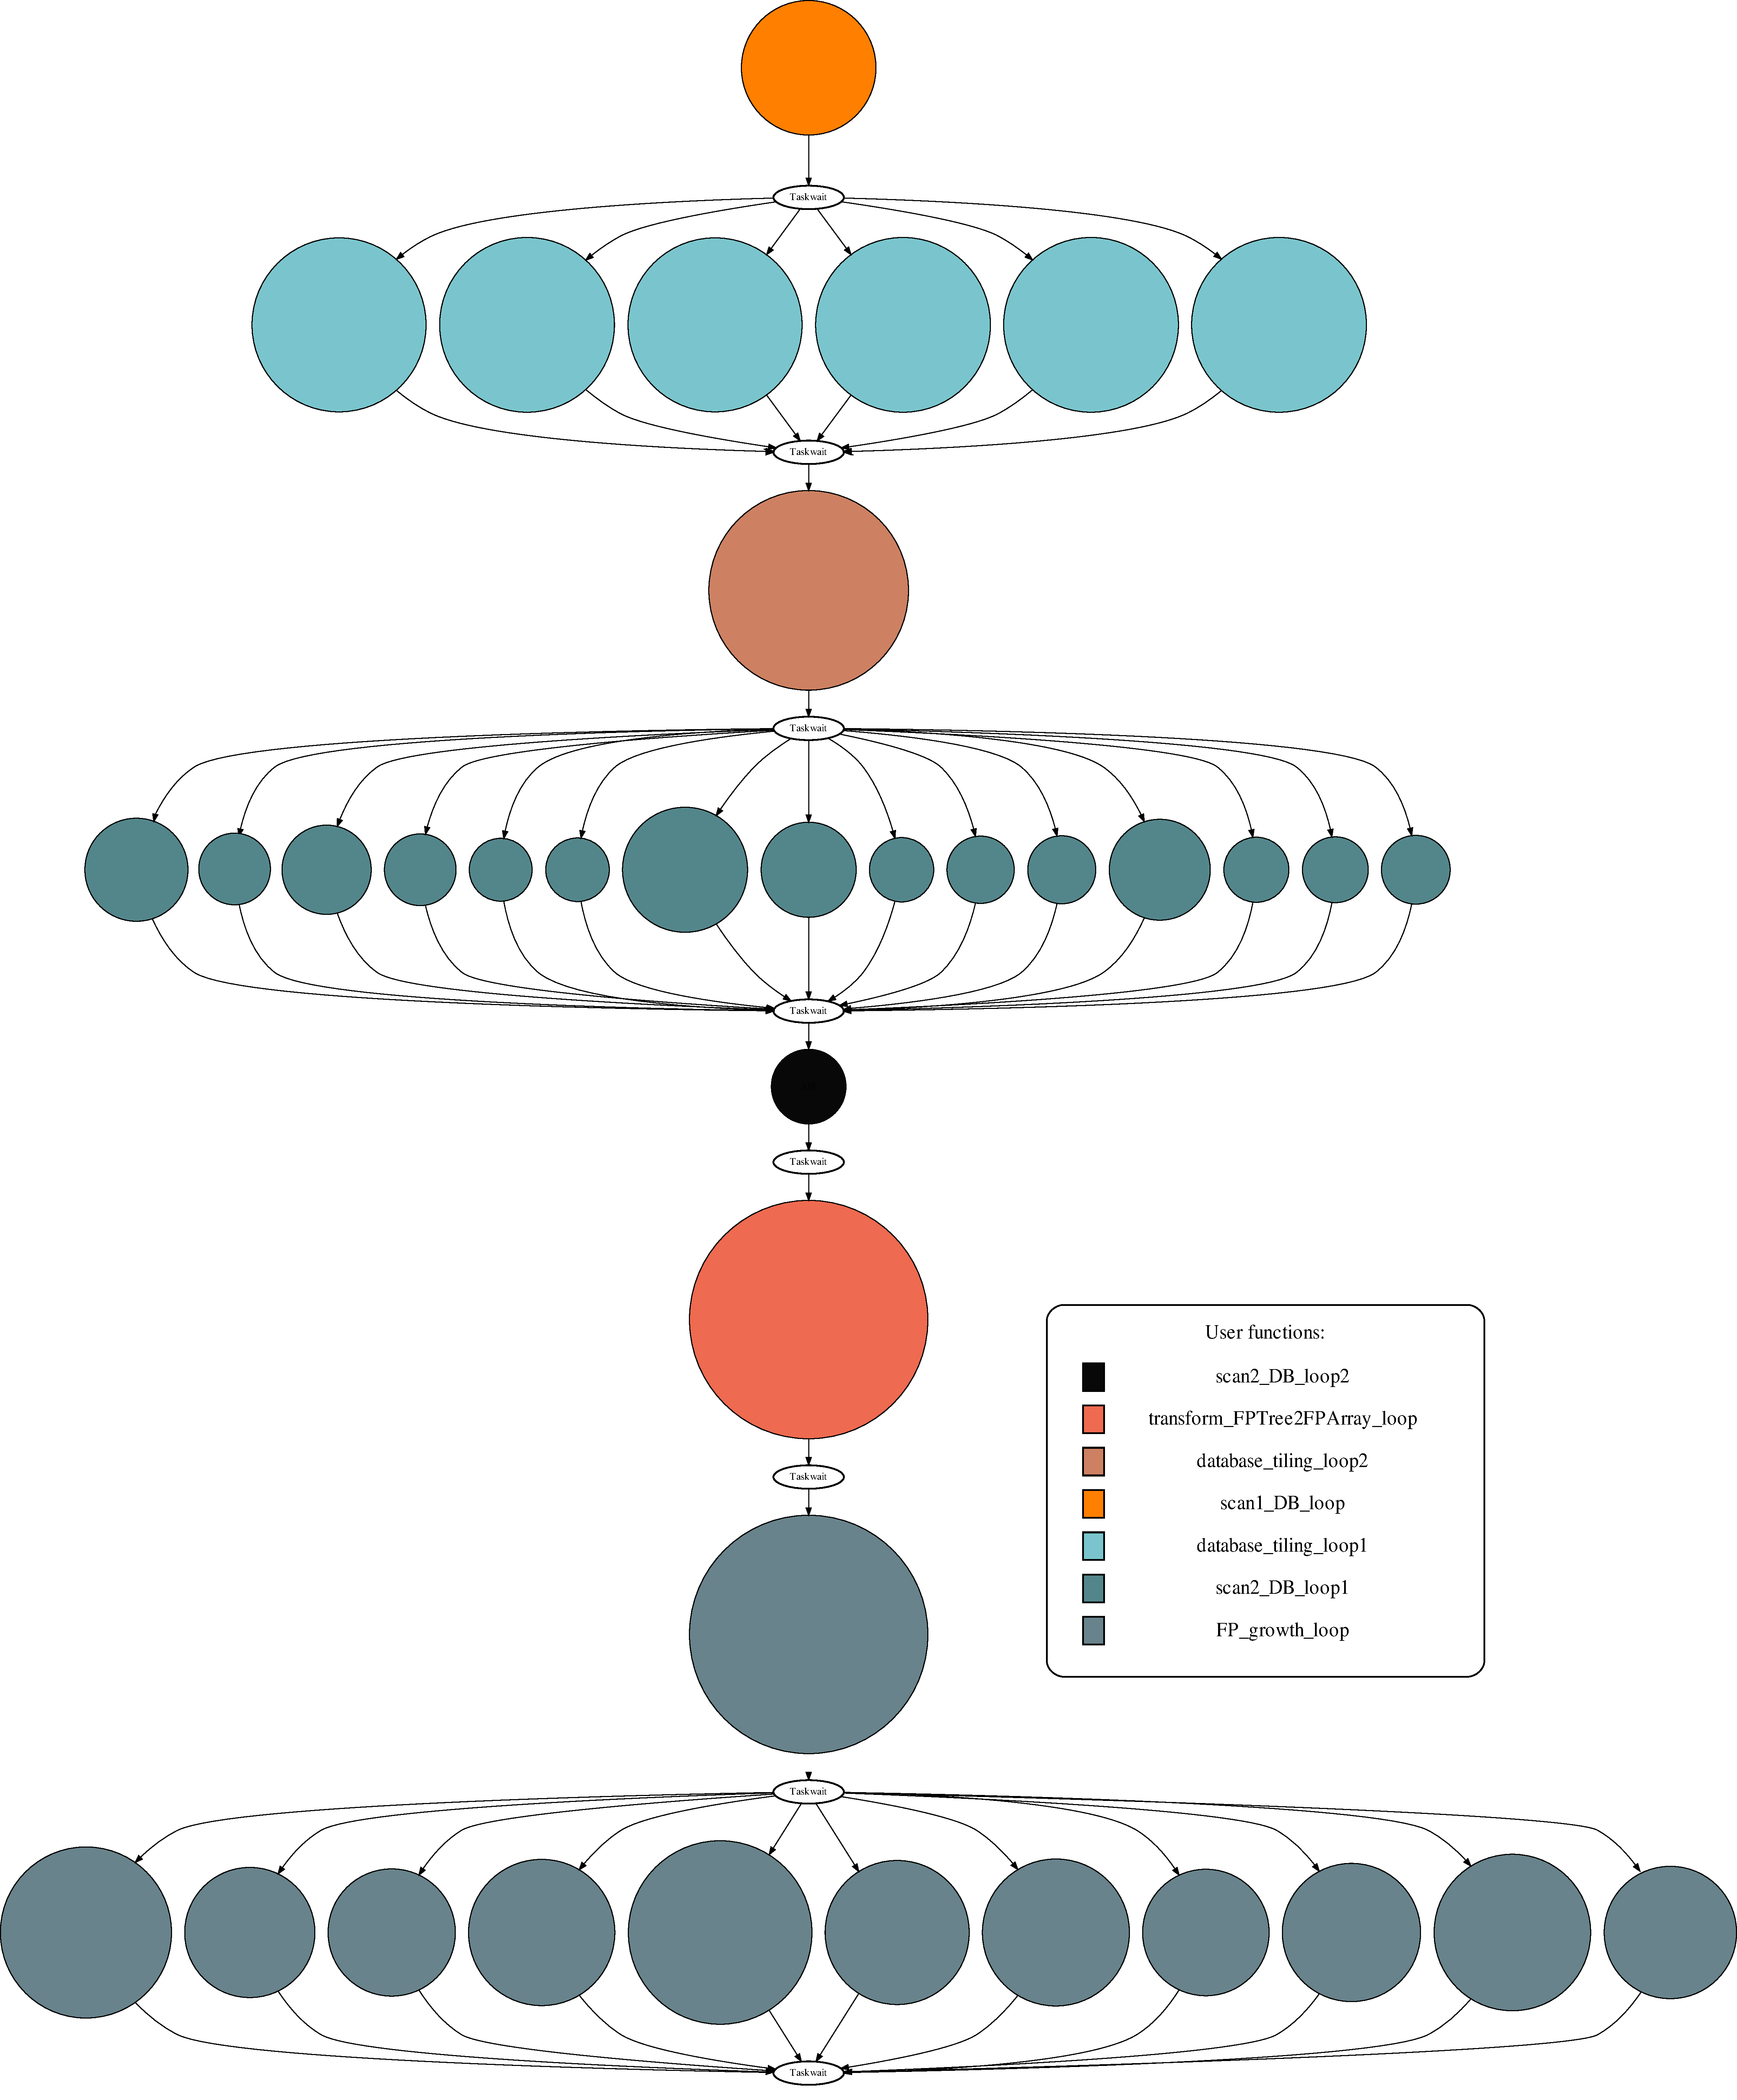
\includegraphics[width=.8\columnwidth]{ifcg/figures/freqmine_taskgraph}%
	\caption{Task-graph of freqmine application.  Edges represent data dependencies among
tasks.}
	\label{fig:freqmine_tg}%
	\vspace{.5cm}
\end{figure}

\paragraph{\textbf{Freqmine}}
Data mining application that makes use of an array-based version of the Frequent Pattern
(FP) growth method for Frequent Itemset Mining~\cite{conf/fimi/GrahneZ03}.

\paragraph{\textit{Pthreads}}
The application uses a compact tree data structure, denoted \emph{FP-tree}~\cite{Han:2000:MFP:335191.335372}, to store information about frequent patterns of the transaction database.  The FP-tree is coupled with a header table, which is a list of database items, sorted by decreasing order of occurrences.
The FP-growth algorithm traverses the FP-tree structure recursively, constructing new FP-trees until the complete set of frequent itemsets is generated.
There are three parallel kernels.  The \texttt{Build\_FP-tree\_header\_table} kernel performs a database scan 
and counts the number of occurrences of each item.  The result is the FP-tree header table.   
\texttt{Build\_Prefix\_tree} kernel performs a second database scan required to build the prefix tree
and the \texttt{Data\_Mining} kernel obtains the frequent itemset information by using the previous two structures.  It creates
an additional lookup table, which allows faster traversals on sparse itemsets.
The original \PARSEC{} benchmark uses OpenMP2.0 for loop parallelization inside each kernel.  

\begin{figure}[ht!]%
	\center
	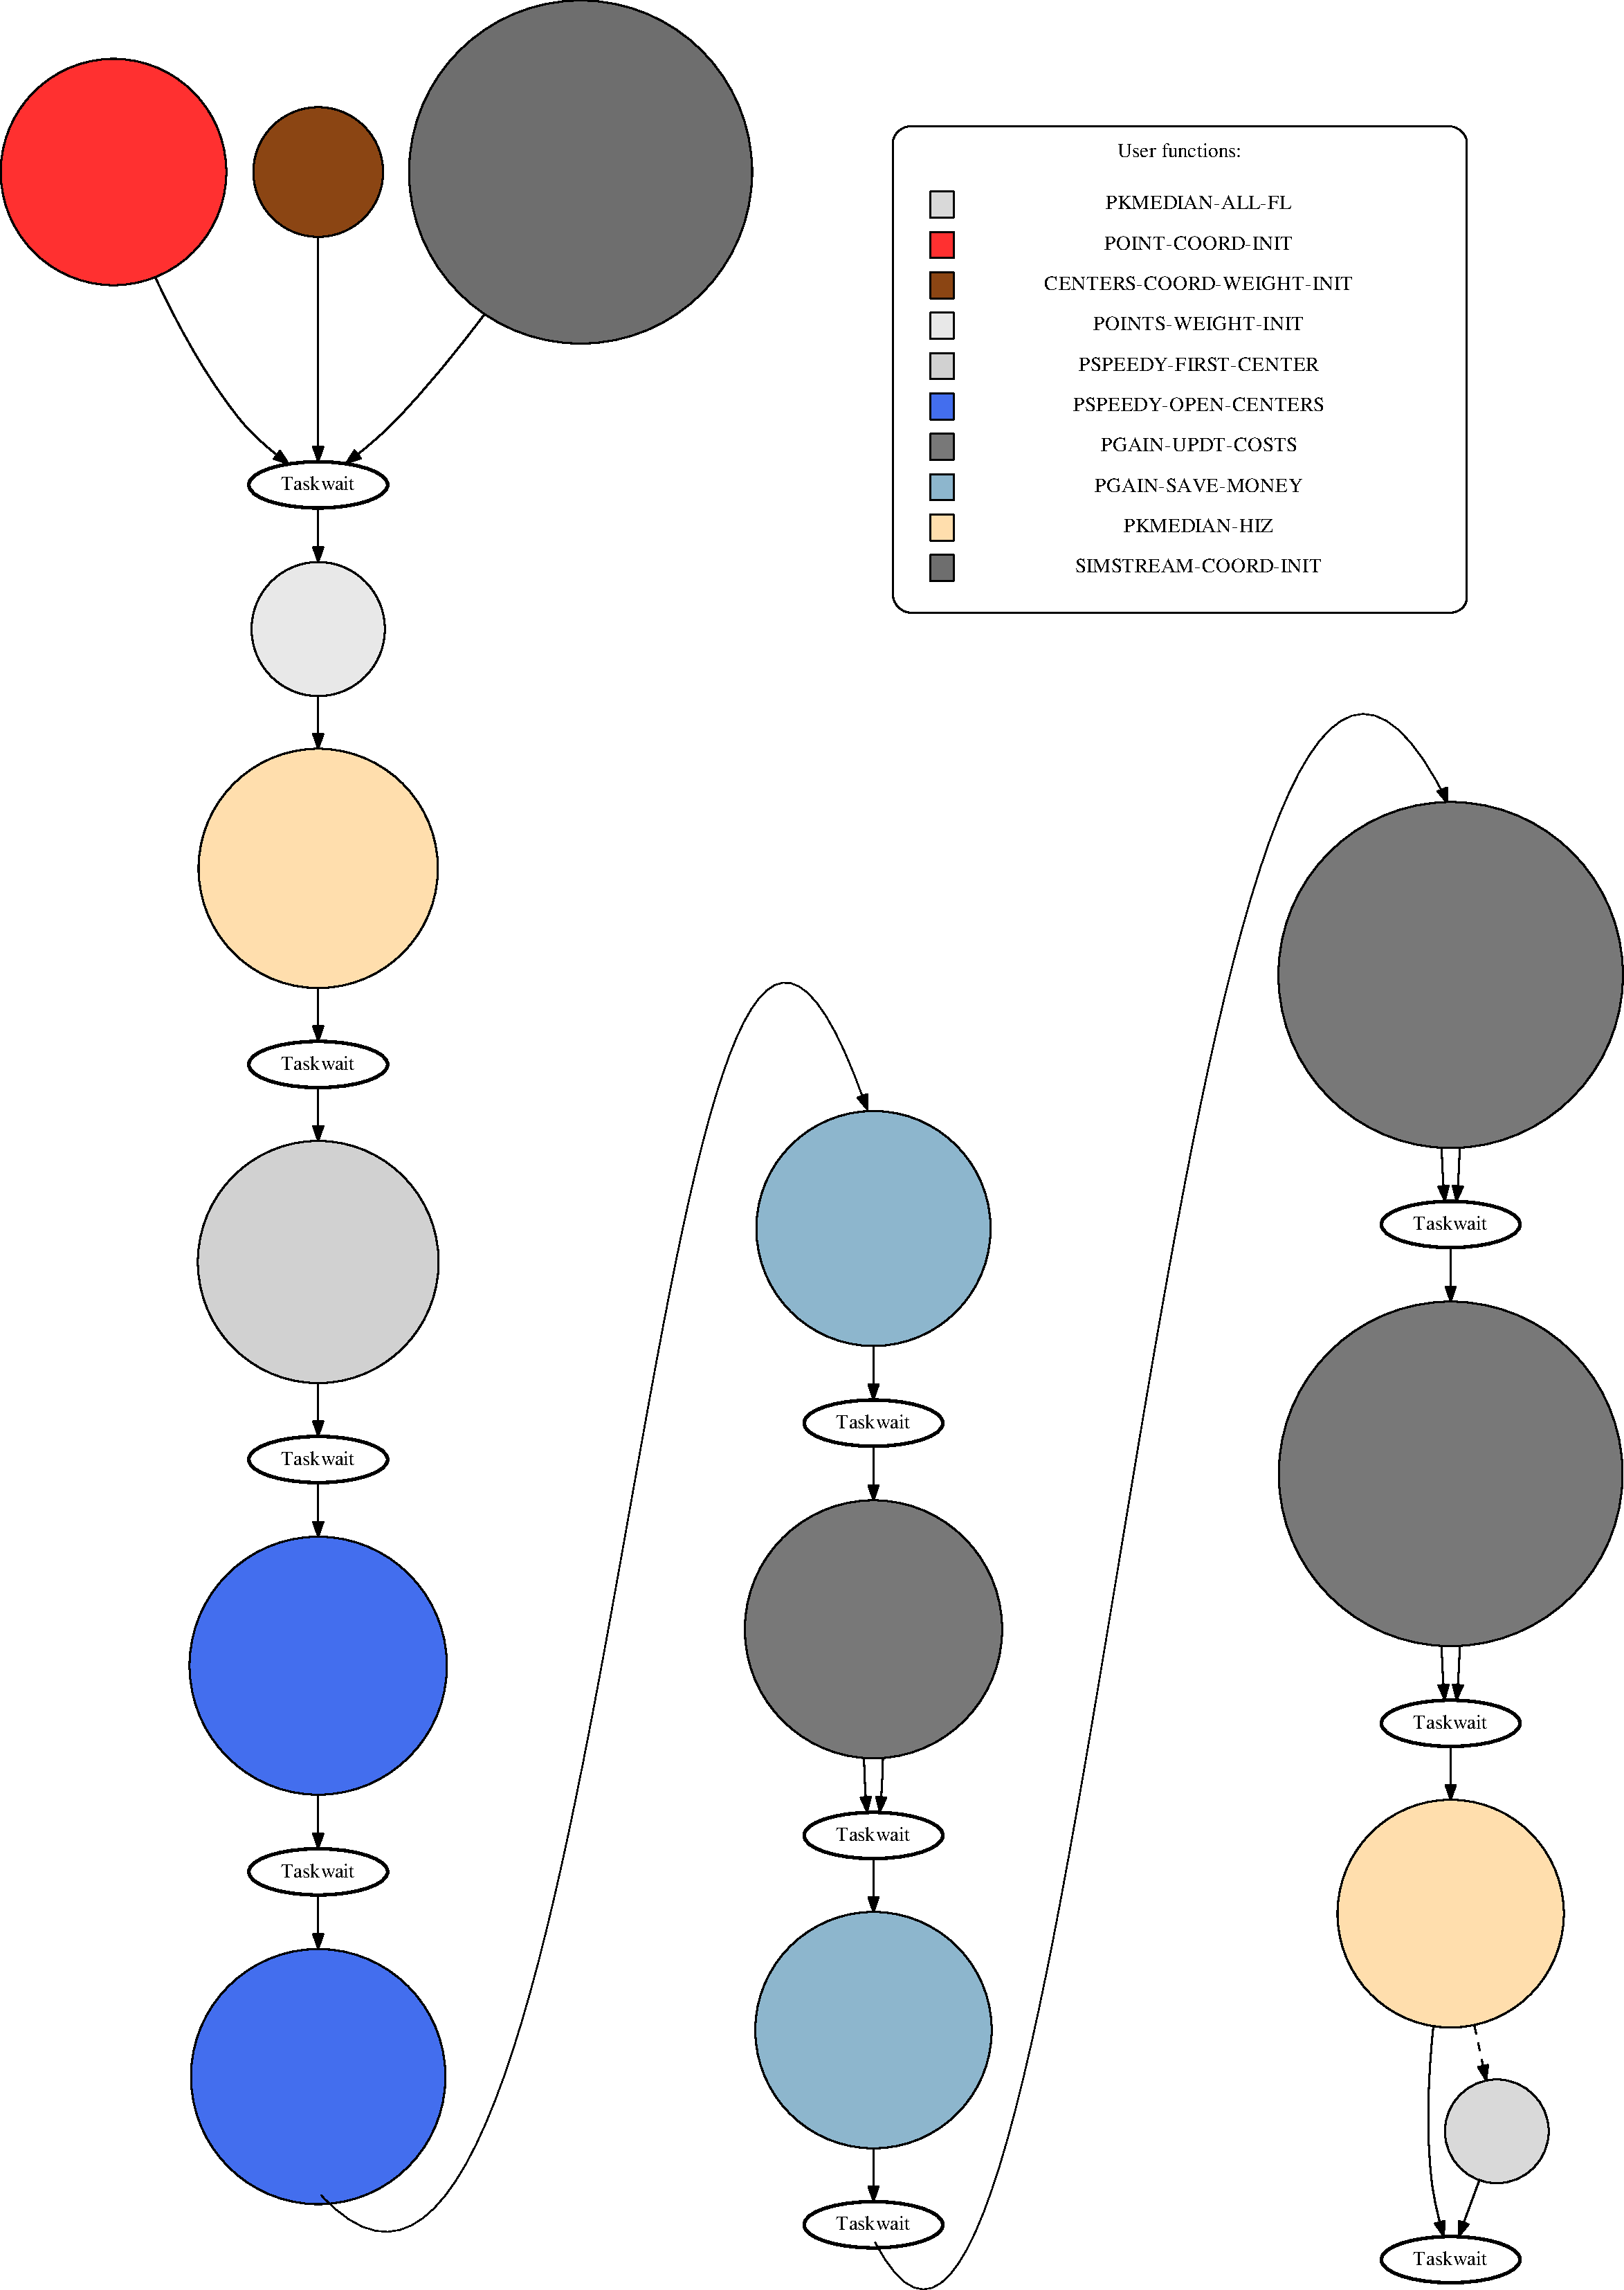
\includegraphics[width=.6\columnwidth]{ifcg/figures/streamcluster_taskgraph}%
	\caption{Task-graph of streamcluster application.  Edges represent data dependencies among
tasks.}
	\label{fig:streamcluster_tg}%
	\vspace{.5cm}
\end{figure}



\paragraph{\textit{Task-based}}
In our implementation we taskify each iteration. We do not use any dataflow relations in this application, and resolve to 
adopt the locking and barrier synchronization used in the original OpenMP version.
The barrier synchronization is shown in the task graph in figure \ref{fig:freqmine_tg}.

\paragraph{\textbf{Streamcluster}}
Streamcluster is a kernel that solves the online clustering problem. 
It takes a stream of points and then groups them in a predetermined number of clusters with their respective centers.  


\paragraph{\textit{Pthreads}}
Up to 90\% of total execution time is spent in function \texttt{pgain}, 
computing whether opening a new center is advantageous or not.  For every 
new point, function \texttt{pgain} calculates the cost of making it a new center by reassigning some points to it and 
comparing it to the minimum distance $d(x,y) = |{x-y}|^2$ between all points $x$ and $y$.
The result is accepted if found to favor the new center.  Data points are statically partitioned by a given block 
size, which determines the level of parallelism in the application. In the Pthreads version this is equal to the number of
threads. 

\paragraph{\textit{Task-based}}
In our implementation we follow a different decomposition strategy, making the number of tasks independent
of the number of partitions.   
Barriers are employed to synchronize accesses
to a partition in both Pthreads and the task-based implementation. 
In the case of Pthreads, an additional user 
implemented library is used for the barriers. 
This library is not required in the case of the OmpSs implementation, as 
the runtime already has a generic barrier implementation.
A task graph of our task-based implementation and the dependencies among tasks is shown in figure \ref{fig:streamcluster_tg}

\paragraph{\textbf{Swaptions}}
Economics application that uses the Heath-Jarrow-Morton (HJM)\cite{RePEc:ecm:emetrp:v:60:y:1992:i:1:p:77-105} for pricing of a portfolio of swaptions. To calculate prices it employs the Monte Carlo simulation.

\begin{figure}[ht!]%
	\center
	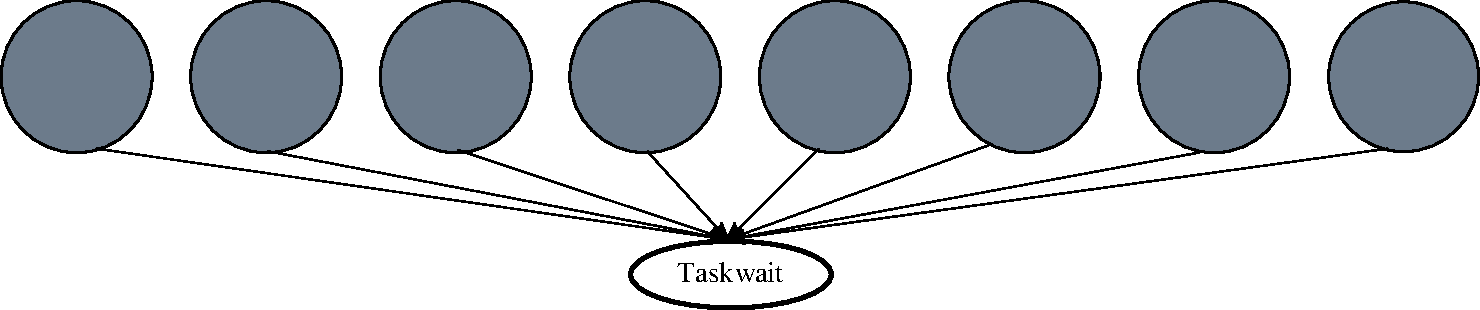
\includegraphics[width=.8\columnwidth]{ifcg/figures/swaptions_taskgraph}%
	\caption{Task-graph of swaptions application.}
	\label{fig:swaptions_tg}%
	\vspace{.5cm}
\end{figure}


\paragraph{\textit{Pthreads}}
The application stores the portfolio into an array. In the Pthreads version, this array is divided by the number of available threads, each thread working on its own part of the array. 

\paragraph{\textit{Task-based}}
We use the exact same strategy, where each task works on a part of the array.  No data dependencies exist between the tasks.
Figure \ref{fig:swaptions_tg} shows the corresponding task graph for the swaptions application.  No dependencies exist between tasks,
synchronization is only achieved through barriers.
%\paragraph{\textbf{x264}}
%An AVC (Advanced Video Coding) video encoder, based on the ITU-T H.264 standard~\cite{H.2642007}.
%It improves over previous video encoding standards at the expense of significantly increased 
%encoding and decoding time.


%The parallel version of x264 extracts parallelism by processing different frames concurrenlty. Initially frames are split in smaller 
%macroblocks of 16x16 pixels.  These macroblocks are processed by a pipeline with a number of stages equal to the number of frames.
%The stages are: \texttt{Read\_frame}, which reads input frames, \texttt{Analyse\_frame}, which creates data dependencies among macroblocks,
%\texttt{Encode\_frame}, which is the encoding state and \texttt{Write\_frame} which writes the encoded frames to the output file.


%The task-based implementation does not use the macroblocks. Instead
%it works on whole frames.  We use two different task types, each spawned for each frame.  The first reads the frame and the second performs the
%three other pipeline stages.  The pipeline stages are synchronized using shared variables. 
 

\section{Programmability}
Different models and languages offer diverse ways to express concepts, such as parallelism or asynchrony.
In this section we evaluate how successful and easy it is to express parallelism using task-based models.  
A good proxy to evaluate how complex a particular implementation is the number of lines of code it takes.
Despite being a metric proposed some decades ago, comparing different programming models in terms of the total number of code lines
is still a valid metric. Indeed, recent publications make an extensive use of it~\cite{Vandierendonck:2011:PPG:2001252.2001265,Dongarra20081}.

%\subsection{Expressiveness}
%\edit{In the Parsec suite we encounter a diverse
%set of parallelization strategies, which however can be grouped into data-parallelism, pipeline parallelism and hybrid between data and pipeline
%parallelism (e.g. \texttt{facesim}).  We were able to express at least the same amount of parallelism in all the 10 benchmarks we used for this study,
%compared to the Pthreads and OpenMP versions.  Additionally, in the cases of \texttt{bodytrack} and \texttt{facesim} we were able to express additional
%parallelism with the use of dataflow annotations and tasks.  Note that in the case of \texttt{dedup}, we adopted a parallelization method with less available
%parallelism than in the case of Pthreads.  We were also able to implement the original Pthreads \texttt{dedup} version but for performance reasons we adopted
%the version with less parallelism.   Section~\ref{sec:implementation} explains this decision in detail.}


%\edit{Although we were able to implement 10 out of the 10 benchmarks, it is possible that we could obtain better results and express additional parallelism in some
%cases, but not with the current standard syntax that OpenMP 4.0 offers.  As discussed in Section \ref{sec:implementation}, the current syntax could benefit from
%extensions that could express data dependencies among irregular and dynamic data structures.  The current OpenMP 4.0 standard is focused on continuous data structures.}

\begin{figure*}[!htbp]
        \centering
        \begin{subfigure}[b]{0.8\textwidth}
                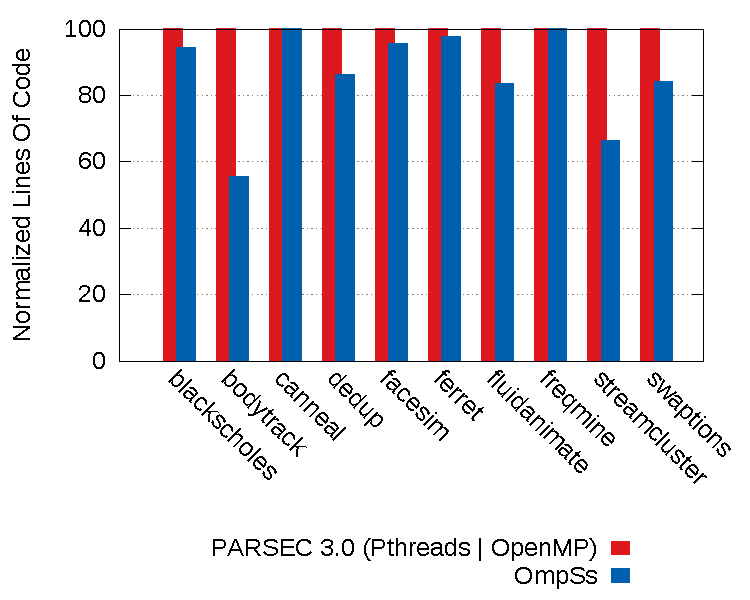
\includegraphics[width=\textwidth]{ifcg/figures/absolute_loc_norm}%
                \caption{Comparison between all source files.}%
                \label{fig:absolute_loc}
                \vspace{0.4cm}
        \end{subfigure}%
				\hfill
        \begin{subfigure}[b]{0.8\textwidth}
        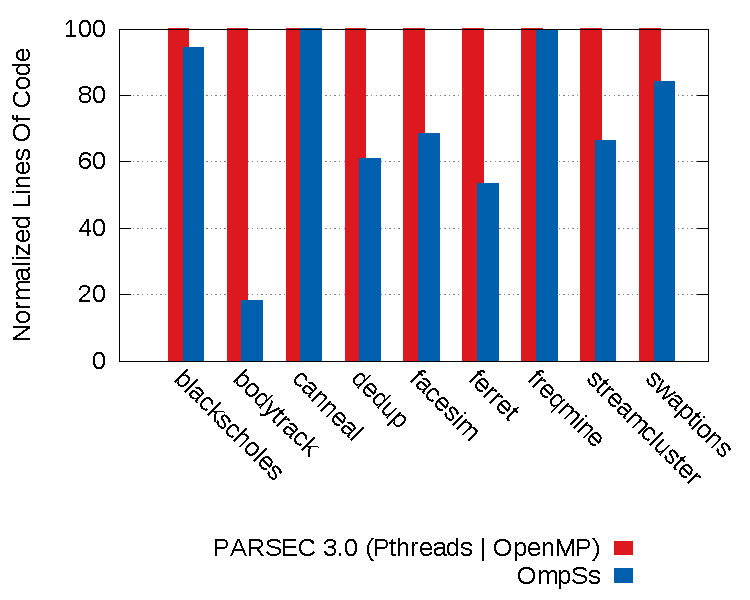
\includegraphics[width=\textwidth]{ifcg/figures/relative_loc_norm}%
        \caption{Comparison between only source files containing parallel code.}%
        \label{fig:relative_loc}%
        \end{subfigure}%
  \caption{Comparison of lines of code between our task-based implementations and the original Pthreads or OpenMP versions.}
        \label{fig:loc_comparison}
\end{figure*}


\subsection{Lines Of Code}
\label{sec:lines}
The reduction of the lines of code (LOC) attests to a more compact and readable code.
%keeping in mind that the actual 
%algorithm complexity remains unchanged.}
In some of our PARSEC task-based implementations, a simple pragma directive replaced application 
specific schedulers, scheduling queues, thread pooling mechanisms and lock synchronization.
We do not change the algorithm in any of the task-based parallel strategy implemented in the PARSEC suite.
Figure~\ref{fig:absolute_loc} shows a normalized comparison between the lines of code of our task-based implementations and the original Pthreads/OpenMP implementations of the PARSEC 3.0 distribution.
The PARSEC 3.0 versions we refer to are always the Pthreads versions, except in the case of \texttt{freqmine} where, since there is no Pthread version available, the OpenMP2.0 version is taken as reference.
We preprocess all source files so that they only contain lines of code relevant to the respective programming model\footnote{PARSEC benchmarks contain mixed serial, Pthreads, OpenMP and TBB source code, and make use of macros to enable conditional compilation for only one programming model at a time.}.
%The LOC column in Table~\ref{tab:parsec} shows the total lines of code for each application, counting all source files.
%Upon careful inspection we can observe that the task-based version requires less lines of code, however parallel code is only a fragment of the sources
%for most applications.  
Figure \ref{fig:relative_loc} shows the total lines of code comparison when we only consider files that are relevant to the parallel 
implementation, that is, files that contain calls to Pthreads or task invocations, asynchronous I/O implementations, atomic primitives, etc.
In this graph we see that the reductions in terms of lines of code of our task-based strategies are significant.
In case of \texttt{bodytrack}, we are able to remove 81\% of the code lines. Since \texttt{Bodytrack} implements its own scheduler to deal with load balancing, there is much room for code reductions by replacing this ad-hoc mechanisms for a few pragma annotations.

By using tasks and dataflow relations, it is very easy to implement pipelines.  We adopt this approach for both \texttt{dedup} and \texttt{ferret}, 
which result in a significant decrease in LOC (38\% and 46\%, respectively). Figure~\ref{lst:ferret-ompss} shows the pipeline code for \texttt{ferret}.  All that is required is
to taskify the different pipeline stages and make sure that dataflow relations force in-order execution of tasks in the same pipeline instance. The Pthreads version requires the implementation
 of queues between each stage, which must also be safe to use by multiple threads and concurrent accesses.
\texttt{Streamcluster} and \texttt{fluidanimate} task-based versions also reduce lines of code by 33\% and 21\% respectively, by removing the need for an additional, user implemented, barrier library. 
\texttt{Blackscholes} and \texttt{swaptions} are relatively simple applications, containing only one do-all parallel loop each.
In these cases the LOC difference is minimal (0.5\% and 15\%, respectively). 
In the cases of \texttt{canneal} and \texttt{freqmine} we see no difference in LOC. 
\texttt{Canneal} is not a data parallel application and in both cases Pthreads and tasks are used merely as thread launching mechanism, while the synchronization effort is essentially the same. 

It is worth noting that conventional synchronization primitives can still be used with tasks, without penalizing the programmer.
\texttt{Freqmine} is implemented in OpenMP, which excels at parallelizing loops with very little effort from the programmer and is the ideal programming model for this application. 
In our implementation we simply taskify the loops, essentially not affecting LOC.
\texttt{Facesim} also benefits from the tasks-based approach by 37\%, as the queues required to schedule work have been 
completely removed. 
Overall, we see that the task-based model reduces code size and by \AVERAGELOC{} on average.



\begin{figure}[p]
        \centering
        \begin{subfigure}{0.8\textwidth}
                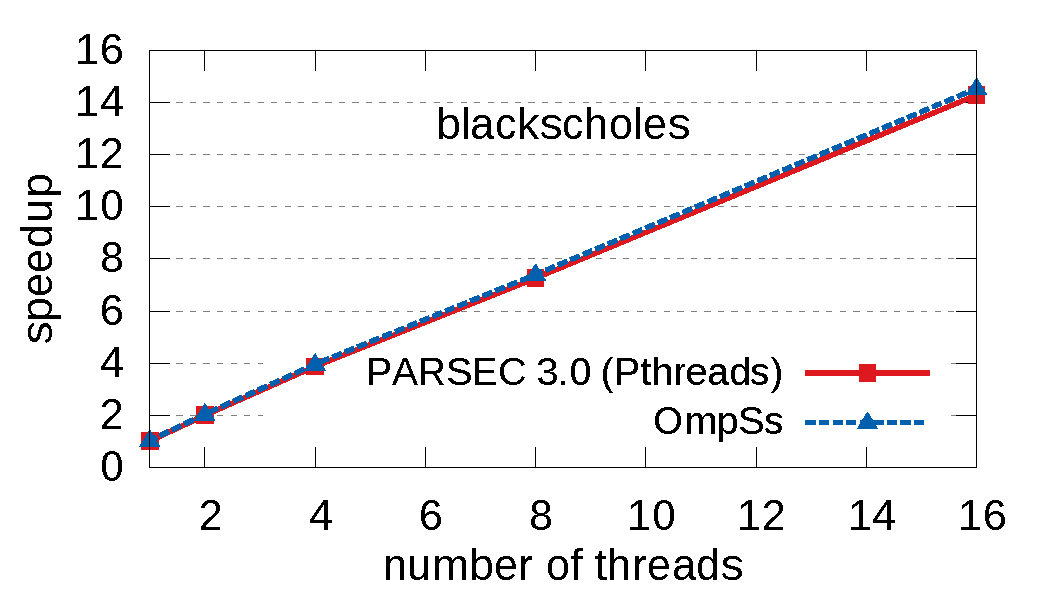
\includegraphics[width=\textwidth]{ifcg/figures/blackscholes_scale}
                \label{fig:blackscholes_scale}
        \end{subfigure}%
\hfill
        \begin{subfigure}{0.8\textwidth}
                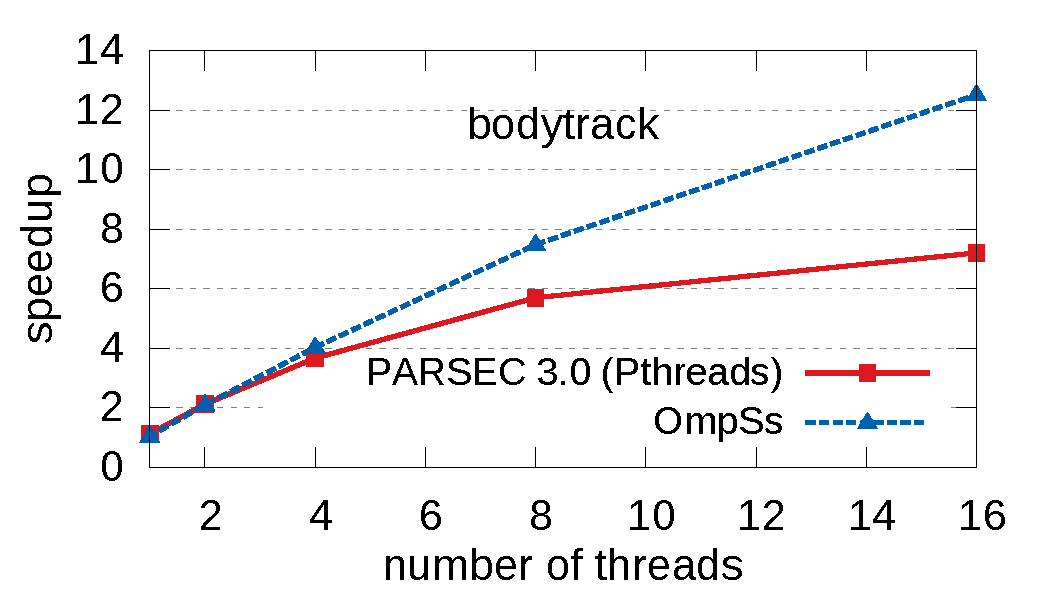
\includegraphics[width=\textwidth]{ifcg/figures/bodytrack_scale}
                \label{fig:bodytrack_scale}
        \end{subfigure}
        
				\begin{subfigure}[b]{0.8\textwidth}
                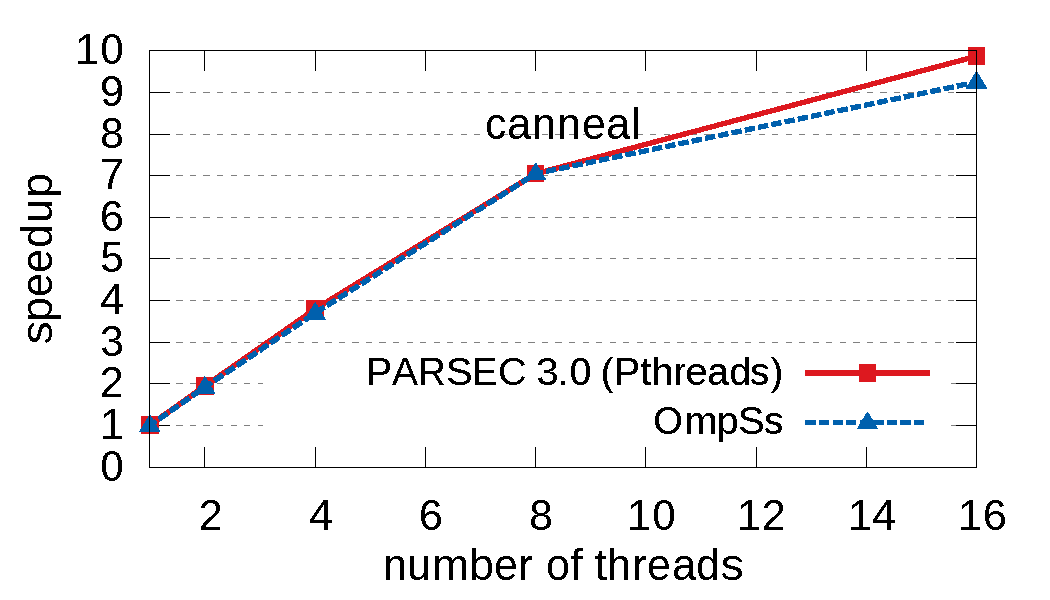
\includegraphics[width=\textwidth]{ifcg/figures/canneal_scale}
                \label{fig:canneal_scale}
        \end{subfigure}
      \caption{Comparison of scalability between the task-based implementations and the original (Pthreads/OpenMP) versions.}
			\label{fig:scalability_graphs_1}
\end{figure}

\begin{figure}[p]
				\centering
        \begin{subfigure}[b]{0.8\textwidth}
                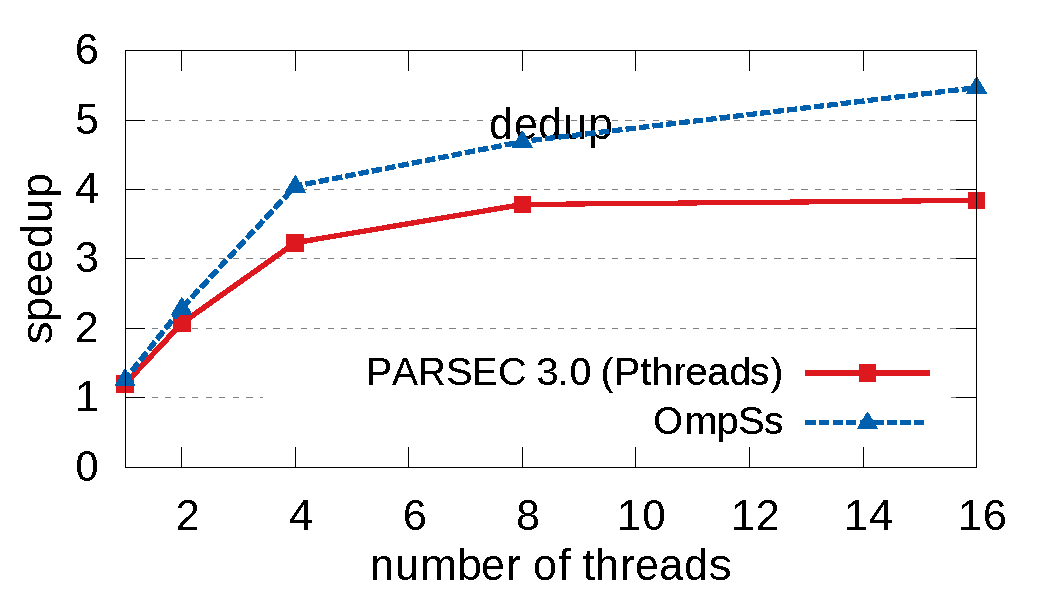
\includegraphics[width=\textwidth]{ifcg/figures/dedup_scale}
                \label{fig:dedup_scale}
        \end{subfigure}
\hfill
        \begin{subfigure}[b]{0.8\textwidth}
                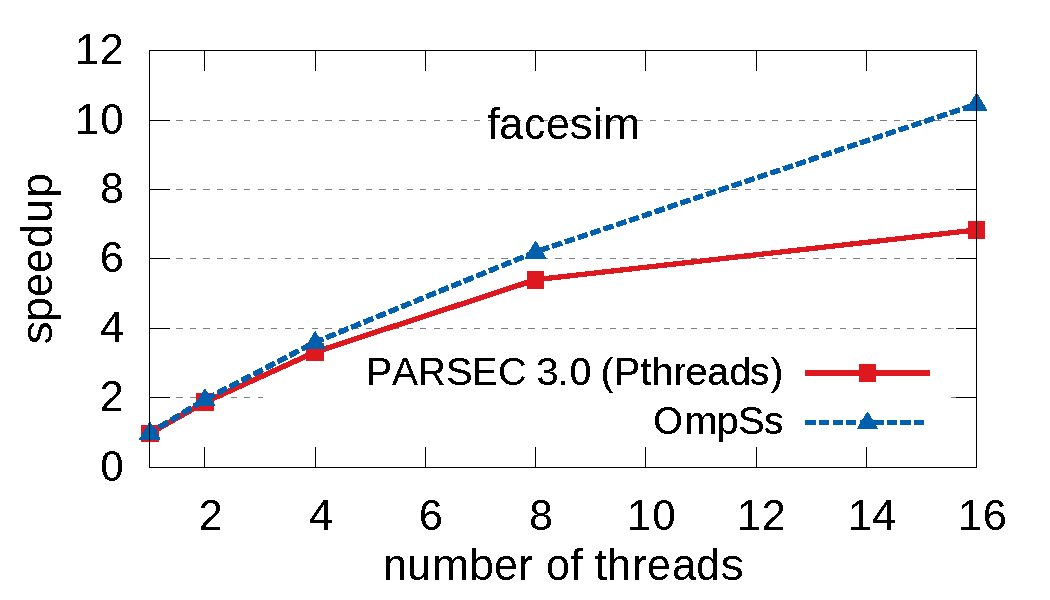
\includegraphics[width=\textwidth]{ifcg/figures/facesim_scale}
                \label{fig:facesim_scale}
        \end{subfigure}
\hfill
				\begin{subfigure}[b]{0.8\textwidth}
                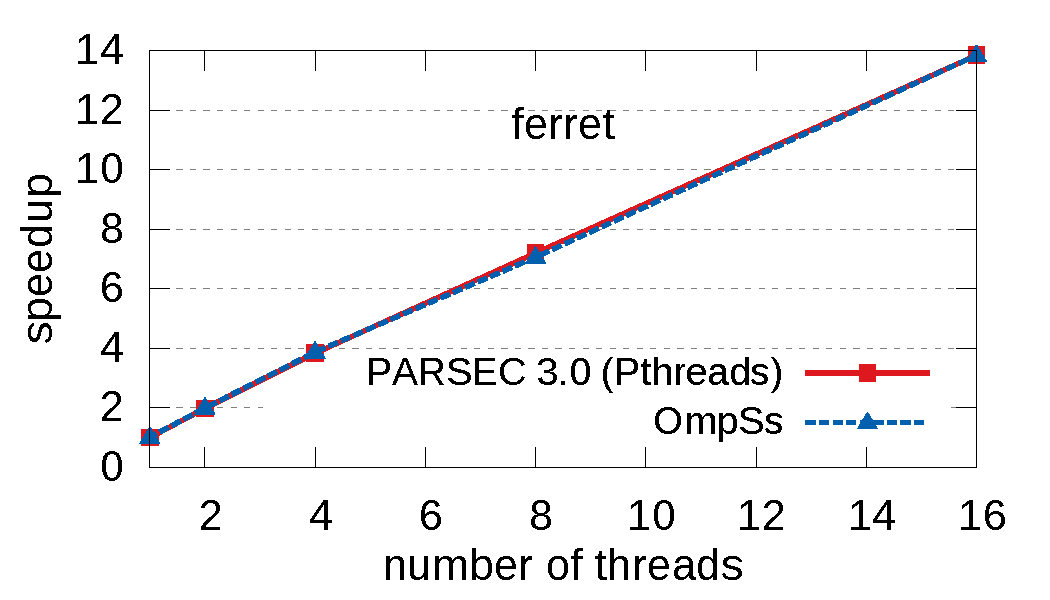
\includegraphics[width=\textwidth]{ifcg/figures/ferret_scale}
                \label{fig:ferret_scale}
        \end{subfigure}%
      \caption{Comparison of scalability between the task-based implementations and the original (Pthreads/OpenMP) versions.}
			\label{fig:scalability_graphs_2}
\end{figure}

\begin{figure}[p]
				\centering
				\begin{subfigure}[b]{0.8\textwidth}
                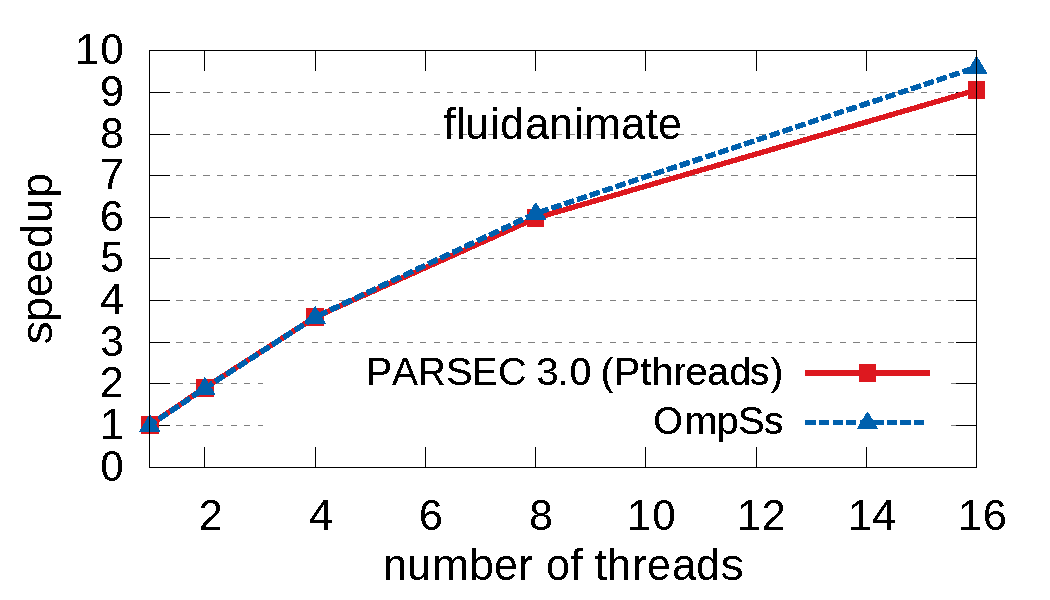
\includegraphics[width=\textwidth]{ifcg/figures/fluidanimate_scale}
                \label{fig:fluidanimate_scale}
        \end{subfigure}
\hfill
        \begin{subfigure}[b]{0.8\textwidth}
                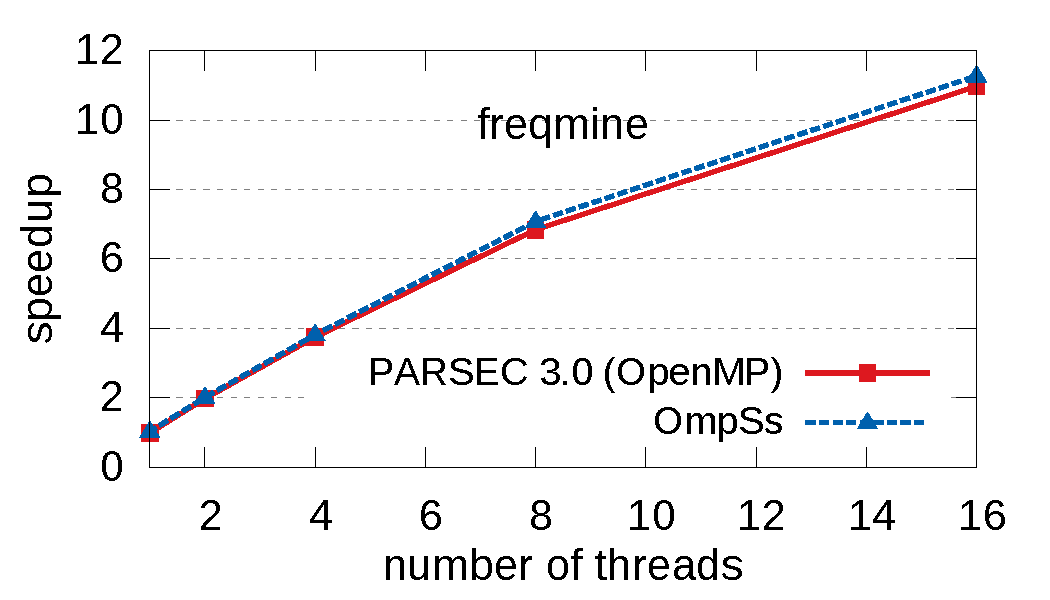
\includegraphics[width=\textwidth]{ifcg/figures/freqmine_scale}
                \label{fig:freqmine_scale}
        \end{subfigure}
\hfill        
				\begin{subfigure}[b]{0.8\textwidth}
                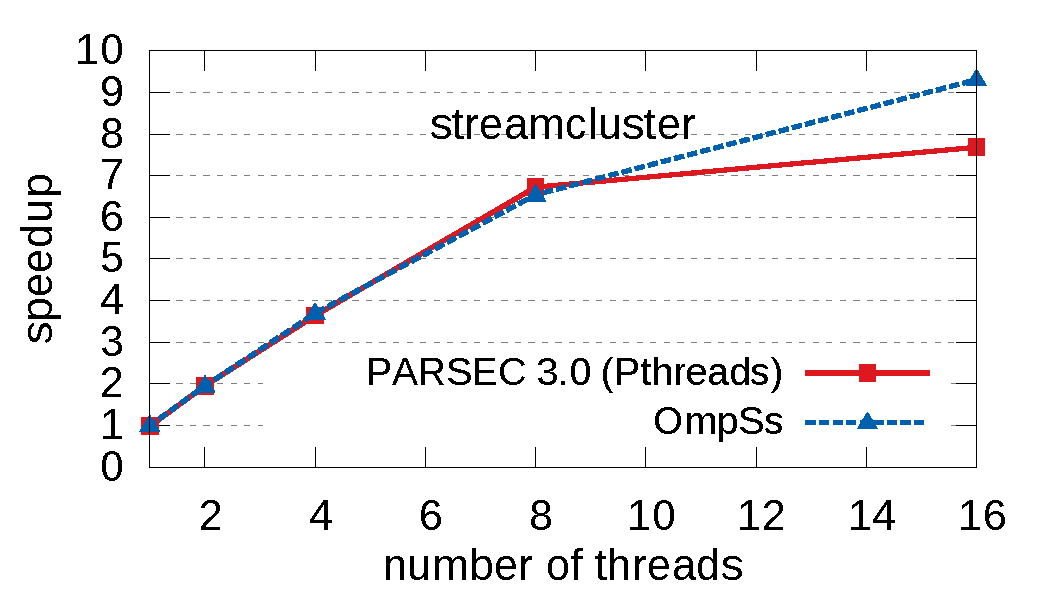
\includegraphics[width=\textwidth]{ifcg/figures/streamcluster_scale}
                \label{fig:streamcluster_scale}
        \end{subfigure}
			\caption{Comparison of scalability between the task-based implementations and the original (Pthreads/OpenMP) versions.}
			\label{fig:scalability_graphs_3}
\end{figure}

\begin{figure}[ht]
				\centering
        \begin{subfigure}[b]{0.8\textwidth}
                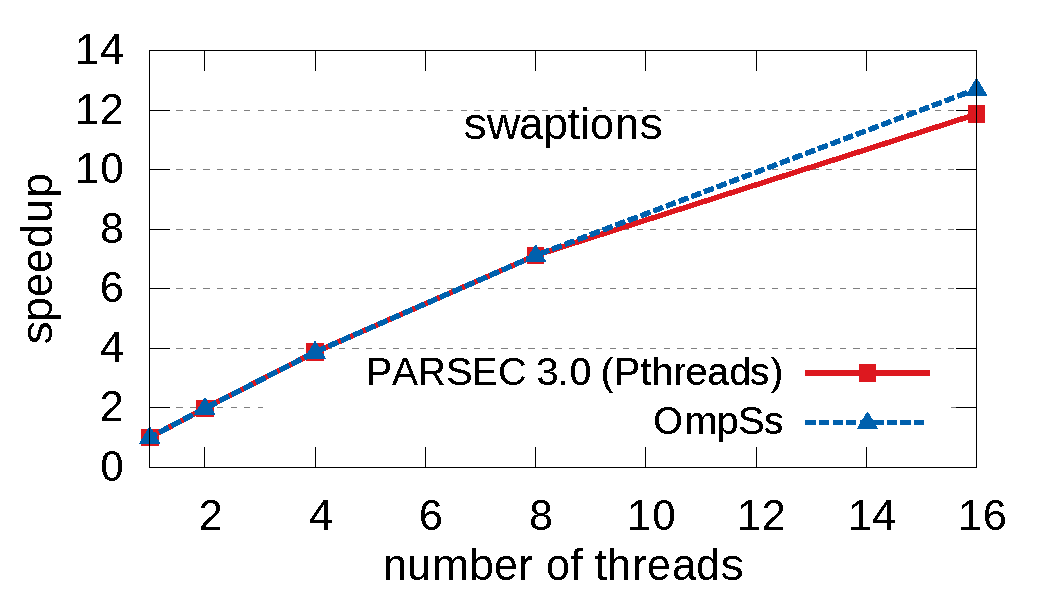
\includegraphics[width=\textwidth]{ifcg/figures/swaptions_scale}
                \label{fig:swaptions_scale}
        \end{subfigure}
      \caption{Comparison of scalability between the task-based implementations and the original (Pthreads/OpenMP) versions.}
			\label{fig:scalability_graphs_4}
			\vspace{.5cm}
\end{figure}





\section{Performance}
\label{sec:task_bench_evaluation}

%Performance is a significant factor when evaluating a parallel programming model.  
In this section we compare our task-based implementations to the original \PARSEC{} implementations in Pthreads or OpenMP.

\subsection{Scalability}
\label{subsec:scalability}
Figures~\ref{fig:scalability_graphs_1},\ref{fig:scalability_graphs_2},\ref{fig:scalability_graphs_3},\ref{fig:scalability_graphs_4} 
shows how the task-based codes scale compared to the \PARSEC{} Pthread/OpenMP versions. 
Results are shown individually per benchmark as we increase the number 
of cores assigned to the application and normalized to the execution time of the serial implementation
\footnote{The PARSEC benchmark suite provides a serial implementation for \texttt{blackscholes}, \texttt{bodytrack}, \texttt{dedup}, \texttt{ferret}, 
\texttt{freqmine} and \texttt{swaptions}. 
For the other benchmarks, the original Pthreads parallel implementation executed on a single core is considered as the baseline.}
 of the application. Nearly all applications scale linearly up to 4 cores.
%However, with 8 and 16 cores, 
%performance improvements diminish.
%reaching 30\%, 42\% and 34\% improvements, respectively.

In the case of \texttt{bodytrack}, as described in Section~\ref{sec:parsecss_implementation}, by concurrently executing different frames, there is always enough work for all threads, while by taskifying the 
output stage of each frame, we overlap this I/O bottleneck with other computation stages. The speedup when run on 16 cores is 12.1x, while the Pthreads implementation reaches a poor 6.8x speedup when run on 16 cores.
The \texttt{dedup} application has a very expensive stage that writes the compressed data to the output file. 
Our task-based implementation is very effective in overlapping this time with computation from the compression stage. Also, the task-based version does not have to reorder the data chunks, 
since the I/O execution takes place in-order as dictated by dataflow relations. This results in an impressive 30\% performance improvement of the OmpSs version with respect to Pthreads when run on 16 cores.
The Pthreads \texttt{facesim} implementation is burdened by barriers that limit available parallelism. 
By using dataflow relations 
%among 
%the different parallel loops and stages, we remove all barriers, except the barriers before starting and finishing the \texttt{CG} kernel,
%which protect the residual calculation. In Section~\ref{sec:implementation} we discuss two different 
%implementations, one only with tasks and one using also OpenMP equivalent loops. Figure\ref{fig:scalability_graphs} shows the speedup for the later version.
%Our initial implementation gave 8.7\% performance improvement compared to the Pthreads version. 
%The issue with our initial approach was that
%some tasks had very high task creation overhead, which led to unfavorable scheduling and load imbalance among threads. 
%We identified some opportunities 
%to overlap computation with task creation, hiding any runtime overheads, but this did not eliminate them completely. By using the loop construct 
%we managed to minimize the task creation overhead. 
we taskify sequential segments of significant cost we effectively
synchronize them with parallel sections preceding and following it.
The performance improvements comes from the overlap of sequential computations with parallel sections.
The task-based parallelization of \texttt{facesim} reaches a speedup of 10.2x when run on 16 cores, while the PARSEC code only reaches a 6.4x speedup.

In the cases of \texttt{blackscholes}, \texttt{canneal}, \texttt{ferret}, \texttt{fluidanimate}, \texttt{freqmine} and \texttt{swaptions}, the Pthreads/OpenMP
versions already achieve good scalability results. With the exception of \texttt{ferret}, the task-based codes have very close resemblance to their Pthreads/OpenMP counterparts, and have offered reduced 
opportunities for \OMPSS{} to dynamically exploit additional parallelism.  
The parallel implementation in these applications, with the exception of \texttt{ferret}, is limited to parallel do-all loops with 
barrier synchronization, essentially exploiting the same amount of parallelism among all versions (OmpSs/Pthreads/OpenMP). 

In the case of \texttt{ferret}, although the code is substantially different, both versions employ the same pipeline model and deliver the same level of parallelism, which is already  high in the Pthread version.  
We express 
a bit of extra parallelism by extending the pipeline with multiple stages, which write to the output file, effectively overlapping some communication with computation. 
However, the final impact in the 
total execution time is limited as the time needed to write the output file is a very small fraction of the total execution time. 
Finally, we observe performance gain (18\%) in \texttt{streamcluster}, which can be partly attributed to the more efficient 
barrier implementation of \OMPSS{}, when compared to the user implemented barriers of the Pthreads version. 
However, the most important performance drawback 
that the original Pthreads implementation suffers from, is the negative NUMA effects.
This issue is observed when we run our experiments on a two socket system.
The Pthreads code partitions the working set by the number of available cores.
We employ a different partition scheme to counter the 
NUMA effects. Through experimentation we observe that the best results can be obtained when using 80 blocks. 

%However, when we use the 
%same number of partitions as the Pthreads version, which is 16, we obtain a moderate speedup of 9\%.  We can observe how the 
%same results in figure~\ref{fig:granularity_comparison}.  Green bar represents the task-based version 
%that uses the same granularity as Pthreads, while the blue bar shows the performance of \texttt{streamcluster}, when using 80 blocks.

\begin{figure}[t]
  \centering
  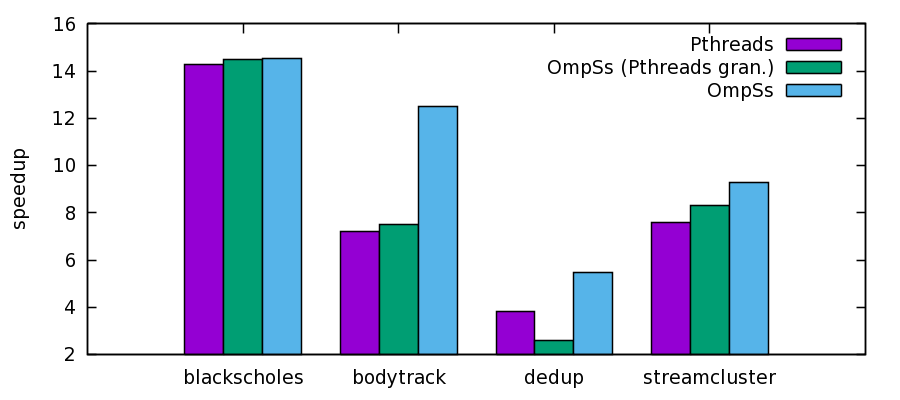
\includegraphics[width=.9\textwidth]{ifcg/figures/parsec_comparison}
  \caption{Speedup comparison for Pthreads and OmpSs with the same granularity, as well as our optimized OmpSs version, when run on 16 cores. Results are normalized to the sequential version of the original code.}
  \label{fig:granularity_comparison}
	\vspace{0.5cm}
\end{figure}

\subsection{Task Granularity Impact}
The granularity of individual tasks is an important factor that needs to be considered when parallelizing an application.
Small task granularity can reduce load imbalance  
but such performance benefits can be neglected by the overhead of the runtime system, as it has to create and schedule more tasks.
Results in Section~\ref{subsec:scalability} show how tuning the task granularity brings performance benefits in some cases (\texttt{blackscholes}, \texttt{bodytrack}, \texttt{dedup} and \texttt{streamcluster})
while in others it is better to keep the same parallel granularity as the \PARSEC{} distribution codes (\texttt{canneal}, \texttt{facesim}, \texttt{ferret}, \texttt{freqmine} and \texttt{swaptions}).
 
In order to provide a more comprehensive comparison, this section examines the performance 
of \texttt{blackscholes}, \texttt{bodytrack}, \texttt{dedup} and \texttt{streamcluster} when using exactly the same granularity as in the \PARSEC{} distribution code.
Figure~\ref{fig:granularity_comparison} shows the speedup of these benchmarks when run on 16 cores. 
The purple bar shows the speedup of the Pthreads version, the green one shows the speedup of a task-based implementation that has the same parallel granularity as its Pthreads counterpart.
Finally, the light blue bar shows the speedup of the optimal task-based implementations discussed in Sections~\ref{sec:parsecss_implementation} and~\ref{subsec:scalability}. 

For the cases of \texttt{blackscholes} and \texttt{streamcluster} the parallelization scheme followed in the three codes (Pthreads and the two OmpSs versions) is the same. 
The difference between the two OmpSs versions is the granularity of the block sizes that are processed per task.
In case of \texttt{blackscholes}, the OmpSs implementation with the same granularity as Pthreads does not perform better since the parallelism of this benchmark follows a fork-join model.
In the case of \texttt{streamcluster}, the task-based implementations always improve the Pthreads performance, even if they operate following the same parallelization scheme and granularity as the Pthreads version.
These improvements come from the NUMA effects correction that the OmpSs versions carry out.

In the case of \texttt{bodytrack} the optimal OmpSs implementation follows a quite different parallelization scheme than the original Pthreads code, as explained in Section~\ref{sec:parsecss_implementation}. 
We consider a trivial implementation in OmpSs where we follow the same parallelization strategy as in Pthreads. 
As shown in Figure~\ref{fig:granularity_comparison}, we do not observe any significant difference in performance among Pthreads and the equivalent OmpSs implementation. 
However, the new parallelization scheme is not applicable to Pthreads as it requires to synchronize the workload by explicit dependencies, which are not available in the Pthreads API.

In the case of \texttt{Dedup}, the trivial Pthreads-like implementation performs poorly, achieving a speedup of 2.6x. 
In this implementation, each pipeline stage is taskified following the Pthreads approach. 
Each large chunk is partitioned into smaller chunks, that will spawn three new tasks (\texttt{Compress}, \texttt{Deduplicate}
and \texttt{WriteOutput}). 
This level of granularity creates hundreds of thousands of tasks, increasing the runtime's overhead significantly. 
In contrast, the optimized task-based version operates at the granularity of the large chunks, creating only a few hundreds of tasks, effectively reducing the runtime overhead. 
%The number of tasks is not the only factor that can influence performance, as their duration is also important. In the fine grain task-based version, some tasks take a very short time to execute. 
%For example \texttt{Deduplication} tasks simply try to insert a single new chunk in a hashtable.

%In general, when following the exact same parallelization strategy and task granularity, Pthreads and OmpSs obtain very similar performance. However, the number of tasks and their size can negatively impact the overall performance. Consequently, users should avoid flooding the runtime system with tasks that run for very short time. Finally, the asynchronous nature of task-based programming models and their programmability allows the users to tune the parallelization strategy or implement more advanced techniques that lead to better final performance.
In some cases, OmpSs can over-perform Pthreads even if the same parallelization scheme and granularity is followed, like the \texttt{streamcluster} results demonstrate.
In some other cases (\texttt{dedup} and \texttt{bodytrack}), the performance improvements come from an optimized parallelization scheme.
Such new schemes could be hardly implemented in Pthreads since they require a direct synchronization via explicit dependencies, which is not available in the Pthreads API.
Finally, in case of simple fork-join applications (i. e. \texttt{blackscholes}) our performance benefits just come from further optimizing the parallel granularity.


\begin{figure*}[p]
  \centering
  \begin{subfigure}{0.75\textwidth}
                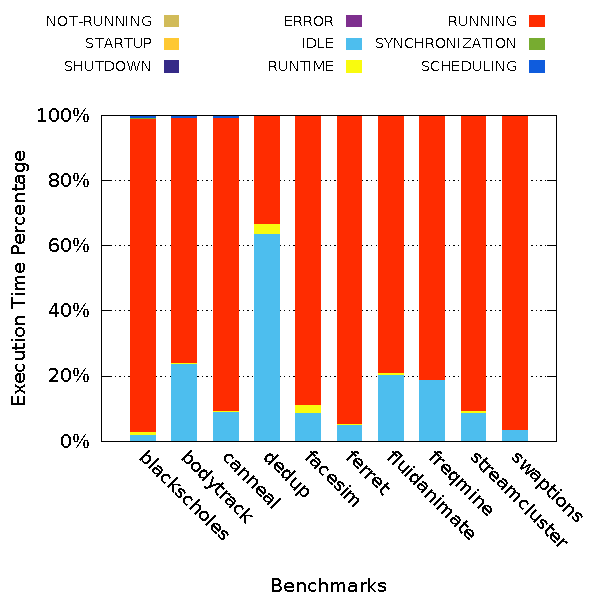
\includegraphics[width=\textwidth]{ifcg/figures/worker-runtime-breakdowns-8}
                \caption{Average time over 8 threads}
                \label{fig:runtime_breakdown_8}
  \end{subfigure}
	\hfill
  \begin{subfigure}{0.75\textwidth}
                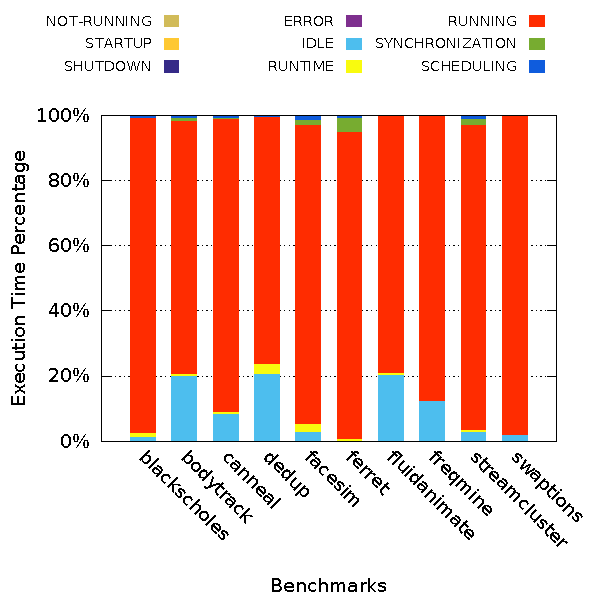
\includegraphics[width=\textwidth]{ifcg/figures/master-runtime-breakdowns-8}
                \caption{Main thread runtime breakdowns}
                \label{fig:master_runtime_breakdown_8}
  \end{subfigure}
        \caption{Runtime breakdowns when running on an 8-core configuration.}
        \label{fig:runtime_breakdown}
	\vspace{.5cm}
\end{figure*}



%\vspace{-0.8cm}
\subsection{Runtime System Overhead}
%\vspace{-0.15cm}
Task creation, scheduling and data dependencies tracking are all handled by the OmpSs runtime system. In this section, we evaluate the impact of these activities over the final parallel performance.
Figure~\ref{fig:runtime_breakdown_8} shows a breakdown of the total execution time of each application. 
Each bar shows the breakdown of one application after averaging the values over eight concurrently executing threads.
The red color represents the portion of time dedicated in running tasks, that is, in running user code. 
All applications, excluding dedup, spend more than 75\% of time doing useful work. 
The cyan bar represents idle time, 
which corresponds to the time a thread is waiting for some work to become available and is caused by load imbalance and sequential code phases. 
In most cases this time is low, except for \texttt{dedup},
where it reaches 60\% of the total execution time. 
In Figure~\ref{fig:runtime_breakdown_8} we also represent the time spent in other activities like synchronization, scheduling, etc. 
None of these activities represent more than 5\% of the total execution time.

Figure~\ref{fig:master_runtime_breakdown_8} shows the same breakdown of execution time but only for the main
thread of execution, which is the one that runs serial parts of the code besides parallel tasks.
\texttt{Dedup} has significantly lower idle time in the main thread, which indicates that there is not enough parallel work to keep all                                                        
threads busy.
This issue has been previously reported~\cite{Vandierendonck:2013:DSP:2503210.2503233}.
In general we see that the overhead of the runtime system is low, with only a few cases that show some time spent in synchronization, scheduling, 
and miscellaneous runtime overhead (in light yellow).
Synchronization time can be time spent waiting a barrier or acquiring/releasing locks. Scheduling includes time needed to resolve dependencies 
and make scheduling decisions, while other runtime overheads are related to activity that cannot be associated with task scheduling and creation.
Overall, we have seen that our implementations improve scalability considerably (by \AVERAGEPERF{} on average), while runtime overhead remains low.

\begin{table*}[!t]
        \centering
        \scriptsize
        \caption{\PARSEC{} parallelization model and properties characterization.}
				\def\arraystretch{1.5}%
				\begin{tabular}{|l|c|c|c|c|c|}
        \hline
        \textbf{Benchmark} & \multicolumn{1}{|c|}{\textbf{Parallel Model}} & \multicolumn{1}{|c|}{\textbf{I/O Heavy}} & \multicolumn{1}{|c|}{\textbf{Synchronization}} & \multicolumn{1}{|c|}{\textbf{LOC Reduction}} & \multicolumn{1}{|c|}{\textbf{Perf. Impr.}}\\
        \hline \hline
        blackscholes & data-parallel & \xmark & dataflow & 5.4\% & 0\% \\ \hline
        bodytrack & pipeline & \cmark & dataflow & 81\% & 42\% \\ \hline
        canneal & unstructured & \xmark & locks/atomics & 0\% & -6.2\% \\ \hline
        dedup & pipeline & \cmark & dataflow/locks & 38\% & 30\% \\ \hline
        facesim & pipeline & \xmark & dataflow/barrier & 31\% & 34\% \\ \hline
        ferret & pipeline & \xmark & dataflow & 46\% & 0\% \\ \hline
        fluidanimate & data-parallel & \xmark & dataflow/barrier & 21\% & 5.7\% \\ \hline
        freqmine & data-parallel & \xmark & barrier/locks & 0\% & 2.7\% \\ \hline
        streamcluster & data-parallel & \xmark & dataflow/barrier/atomics & 33\% & 18\% \\ \hline
        swaptions & data-parallel & \xmark & dataflow & 15\% & 6.6\% \\ \hline
        \end{tabular}
        \label{tab:parsec_characterization}
		\vspace{.5cm}
\end{table*}

\subsection{Characterization of the Applications}
In Table~\ref{tab:parsec_characterization} we characterize the considered applications in terms of parallelization
model, I/O intensity and synchronization scheme. The table also shows code reductions and performance
improvements achieved on a 16-core Sandy Bridge system.
This table summarizes the properties of applications that make them good candidates for adopting a task-based model.

Applications characterized as data-parallel are limited to loop parallelism, where tasks are merely emulating an OpenMP loop construct.
In these cases there is no performance gain, and the programming effort involved either with Pthreads, OpenMP or tasks, is similar. 
Pipeline
applications are better candidates since they separate the application into discrete abstract stages. 
Implementing this paradigm with
tasks implies taskifying the functionality of each stage and describing the data or control dependencies between them. 
In Pthreads, the
programmer has to implement application specific thread pools and queuing systems to achieve the same performance.
Also, task-based models offer in many cases an opportunity to easily
expand the pipeline stages of the application with sequential and I/O intensive codes (e.g. \texttt{facesim} and \texttt{bodytrack} respectively). 
Indeed, by replacing locks and
barriers, the runtime can discover additional dynamic parallelism and eliminate the cost of acquiring locks. 
Our task-based parallelization strategies successfully scale up the pipeline applications with a poorly scaling Pthread version (\texttt{bodytrack}, \texttt{dedup} and \texttt{facesim}) while
reducing the code complexity in all of them.
In case of \texttt{ferret}, the task based version does not perform better than the Pthreads counterpart since its scalability is already very good (14x on a 16-core machine). 
The reduction in terms of lines of code is however dramatic: 46\%.
In the case of
unstructured programs,  e.g. \texttt{canneal}, task based programming does not offer any advantage over threading approaches.  

Overall, we conclude that task-based parallelism can be
effectively used to reduce the effort required to implement pipeline parallelism, while there are also important performance benefits to
be gained if the application has no specific thread pooling mechanisms or I/0 intensive serial regions.
In this scenario, the pipeline can be easily expanded to include the I/0 region and overlap it with a
computation stage of the pipeline.



\section{Summary}

In this Chapter we evaluate the benefits of task-based parallelisim by applying it to the \PARSEC{} benchmark suite.
We discuss and compare our implementations to their
PARSEC Pthreads/OpenMP counterparts. 
We show how task parallelism can be applied on a wide range of applications from 
different domains.   
In fact, by comparing the lines of code between our implementations and the original versions, we make a strong case
that task-based  models are actually easier to use.
The asynchronous nature of task-based parallelism, along with data dependency tracking through dataflow annotations, allows
us to overlap computation with I/O phases.
The underlying runtime system can take care of issues like scheduling and load balancing without significant overhead. 

Our experimental results demonstrate that the task model can be easily applied on a wide range of applications beyond the HPC domain. 
Although, not all applications can benefit from a task-based approach, there are cases where 
it can greatly improve scalability. 
The programs that benefit most are those that present pipeline execution model, where different stages of the application can run concurrently.
The proposed benchmark suite is expected to be of great use in evaluating experimental software
and hardware system designs, offering a more mature testbed compared to the typically used
small kernel applications.


\chapter{Communication Reduction in Deep Neural Network Training}
\label{chap:bitpack}

%\newcommand{\MAXPERF}{42\%}
%\newcommand{\AVERAGEPERF}{13\%}
%\newcommand{\MAXLOC}{81\%}
%\newcommand{\AVERAGELOC}{28\%}

\section{Introduction}
The use of Deep Neural Networks~(DNNs) is becoming ubiquitous 
in areas like computer vision (e.g., image recognition and object detection)~\cite{alexnet, Inception}, speech recognition~\cite{Acoustic}, language translation~\cite{Language}, and many more~\cite{Ciregan2012}. 
DNNs provide very competitive pattern detection capabilities and, more specifically, Convolutional Neural Networks~(CNNs) classify very large image sets with remarkable accuracy~\cite{Krizhevsky2012}.
Indeed, DNNs already play a very significant role in the large production systems of major IT companies and research centers, which has in turn driven the development of advanced software frameworks for the deep learning area~\cite{tensorflow} as well as DNN-specific hardware accelerators~\cite{Merolla668,Jouppi2017}. 
As an example, deep learning solutions are being coupled with physical computational models  for solving pattern classification problems in the context of large-scale climate simulations~\cite{Kurth2017}.
Despite all these accomplishments, deep learning models still suffer from several fundamental problems: the neural network topology is determined through a long and iterative empirical process, the training procedure has a huge cost in terms of time and computational resources, and the inference process of large network models incurs considerable latency to produce an output, which is not acceptable in domains requiring real-time responses like autonomous driving.

The DNN training process typically relies on the backpropagation 
procedure~\cite{Werbos74}, which requires solving an optimization problem 
aimed at discovering the values of network weights that better fit the training data.
A possible way to carry out the backpropagation process is the Gradient Descent 
(GD) method~\cite{Press88}, which aims at fitting the weights to the training data by considering, at each iteration, the steepest descent direction in terms of an error function. 
A popular variant of the GD procedure is the Stochastic Gradient Descent 
(SGD) method~\cite{KieferWolfowitz1952}, which computes the gradient against several randomly chosen samples at each iteration. 
Today's common practice to train DNNs is to split the data set into several subsets, called batches, and let each iteration of SGD to compute a descent direction or gradient that contains contributions of all the samples belonging to the same batch.
SGD converges faster than GD since it updates network parameters at the end of each batch once all samples are processed.

To tackle the large amount of Floating Point computations required to train a DNN, GPUs are usually employed~\cite{You17}. 
They exploit the large amount of data-level parallelism of deep learning workloads. 
Although GPUs and other hardware accelerators have been successfully employed to 
boost the training process, data exchanges involving different accelerators may incur 
significant performance penalties. 

This chapter describes and evaluates a method to accelerate the training of DNNs by reducing the cost 
of data transfers across heterogeneous high-end architectures integrating 
multiple GPUs. By relying on DNNs 
tolerance to data representation formats smaller than the commonly used 32-bit Floating Point (FP) standard~\cite{gupta15, flexpoint17}, this chapter describes how to 
dynamically adapt the size of data sent to GPU devices without 
hurting the quality of the training process. 
Our solution is designed to efficiently use the incoming bandwidth of the GPU accelerators.
It relies on an adaptive scheme that dynamically adapts the data representation format required 
by each DNN layer and compresses network parameters before sending them over the parallel system.
This scheme enables DNNs training to progress in a similar rate as if the 32-bit FP format was used.
This chapter makes the following contributions:

\begin{itemize}

\item It proposes the {\it Adaptive Weight Precision (AWP)} algorithm, which 
dynamically adapts the numerical representation of DNN weights during training. 
AWP relies on DNNs' tolerance for reduced data representation formats.  
It defines the appropriated data representation format per each network layer during  
training without hurting network accuracy.

\item It proposes a new {\it Approximate Data Transfer (ADT)} procedure to compress 
DNN's weights according to the decisions made by the AWP algorithm. 
ADT relies on both thread- and SIMD-level parallelism  
and is compatible with architectures like IBM's POWER 
or x86. ADT is able to compress large 
sets of weights with minimal overhead, which enables the large performance benefits of our approach.

\item It evaluates ADT and AWP on 
two high-end systems: The first is composed of two x86 Haswell multicore 
devices plus four Tesla GK210 GPU accelerators and the second system integrates two POWER9 chips and four NVIDIA Volta V100 GPUs. 
Our evaluation considers the Alexnet~\cite{alexnet}, the VGG~\cite{vgg} and the Resnet~\cite{resnet} network models applied to 
the ImageNet ILSVRC-2012 dataset~\cite{imagenet}.
Our experiments report average performance benefits of 6.18\% and 11.91\% on the x86 and the POWER systems, respectively.
Our solution does not reduce the quality of the training process since networks final accuracy is the same as if they had been trained with the 32-bit Floating Point format.
\end{itemize}

Many proposals describe how data representation formats smaller than the 32-bit Floating Point IEEE standard can be applied to deep learning workloads without harming their accuracy~\cite{bottou08, gupta15, Micikevicius2018}.
This chapter presents the first approach that uses reduced data formats to minimize data movement during DNN training.
This chapter is particularly relevant from the high-performance computing perspective since it proposes
a methodology to accelerate DNNs training in heterogeneous high-end systems, which are extensively used to run deep learning workloads~\cite{You17}. 

This chapter is structured as follows:
%Section~\ref{sec:bitpack_background} motivates our proposals. 
Section~\ref{sec:bitpack_adaptive} describes our first contribution, the Adaptive Weight 
Precision algorithm (AWP). 
Section~\ref{sec:bitpack_approx} details the Approximate Data Transfer (ADT) procedure. 
%Section~\ref{sec:bitpack_setup} explains the experimental setup of this chapter. 
Section~\ref{sec:bitpack_evaluation} describes the  
experiments we conduct to evaluate AWP and ADT on three state-of-the-art neural networks. 
%Section~\ref{sec:Relatedworks} describes the most relevant related work.  
Finally, Section~\ref{sec:bitpack_conclusion} summarizes the main conclusions of this chapter.

\section{The Adaptive Weight Precision (AWP) Algorithm}
\label{sec:bitpack_adaptive}
The Adaptive Weight Precision (AWP) algorithm relies on the tolerance of DNNs to data representation formats smaller than the 32-bit Floating Point standard.
Indeed, previous work indicates that,
unlike scientific codes focused on solving partial differential equations or large linear systems,
neural networks do not always require 32-bit representation during training~\cite{bottou08, gupta15}. 
Even more, adding stochastic noise to certain variables during the learning phase
improves DNNs accuracy~\cite{murray94, bishop95, aud13}.
Nevertheless, when facing unknown scenarios in terms of new workloads or parameter settings,
the data representation requirements of DNNs 
are non-trivial to be determined and, to make things more complicated, they may change as the training phase progresses.

\begin{algorithm}%[H]%algorithm* occupies full page
\caption{Adaptive Weight Precision (AWP) Algorithm}
\label{alg:norm}
{\fontsize{9}{9}\selectfont
\begin{algorithmic}[1]
    \State BitsPerLayer := [$B_0, B_1, \hdots, B_{NumLayers}$]
    \Comment List storing the number of bits corresponding to the data representation of each layer
    \State IntervalCounter := [0, 0, $\hdots$, 0]
    \Comment List storing the number of times the relative change rate
             fails to meet the threshold per layer
    \For {batch := 0 \ldots NumBatches}
        \State Apply backpropagation to batch
        \For {layer := 0 \ldots NumLayers}
            %\State $\text{norm}_{batch, layer} := |\text{W}_{batch, layer}|$
            \State $\delta := \frac{(|\text{W}_{batch, layer}| - |\text{W}_{batch-1, layer}|)}{|\text{W}_{batch-1, layer}|}$
            \If {$\delta$ < T}
                \State $\text{IntervalCounter}_{layer}$ +=  1
            \EndIf
            \If {$\text{IntervalCounter}_{layer}$ == INTERVAL}
                \State $\text{BitsPerLayer}_{layer}$ += N
                %\Comment N is the number of bits to increase
                \State $\text{IntervalCounter}_{layer}$ := 0
            \EndIf
        \EndFor
        \EndFor
\end{algorithmic}
}
\end{algorithm}

The AWP algorithm dynamically  
determines data representation requirements per each network layer by monitoring the 
evolution of the $l^2$-norm of the weights.
AWP identifies the number of bits that are needed to represent 
DNNs weights and guarantees the progress of the training process.
AWP assigns the same data representation format to all weights 
belonging to a certain network layer.
The training starts with a relatively small data representation that is independently 
increased for each layer. 
%In other words, the adjustment of the data format 
%monotonically increases the number of bits to store weights.
%In our context, for the set of $n$ weights $\{ w_1 \hdots w_n \}$ belonging to a certain layer, 
%the $l^2$-norm is used in the following way:
%
%\begin{equation*}
%    |W|=\sqrt{\sum_{k=1}^{n} |w_k|^2}, 
%    \quad \mathrm{whereas} \quad 
%    W = 
%    \begin{pmatrix}
%        w_1 \\
%        w_2 \\
%        \vdots \\
%        w_n
%    \end{pmatrix}, \quad k=1,...,n.
%\end{equation*}

Algorithm~\ref{alg:norm} displays a pseudo-code description of AWP.
Once the backpropagation process has been applied to a given batch, AWP iterates over all network layers.
%Per each layer, AWp computes the change rate~$\delta$ and compares it with a threshold~$T$.
%To do so, 
The algorithm computes per each batch and network layer the $l^2$-norm of all its weights' values 
and derives the relative change rate~$\delta$ of the $l^2$-norm 
with regard to the previously processed batch. 
For the batch $i$, the change rate is defined as  
$\delta_i=(|W_i| - |W_{i-1}|)/|W_{i-1}|$, where $W_i$ is the vector of weights 
of a certain layer while batch $i$ is processed. 
Every time the change rate is below a given threshold \textit{T} for a certain 
layer, the algorithm accounts for it by increasing the $IntervalCounter$ parameter.
The algorithm increases $N$~bits of precision if the change 
rate is below \textit{T} during a certain number of batches defined by the parameter
\textit{INTERVAL} 
and sets the $IntervalCounter$ parameter of the corresponding layer to zero.
Section~\ref{sec:evaluation1} describes how we determine the values of parameters \textit{T}, \textit{INTERVAL}, and \textit{N}.
%Once this counter reaches a certain value \textit{INTERVAL} for a certain layer, the algorithm 
%decides to increase the number of bits representing this layer's weights and 
%sets the $IntervalCounter$ variable of the corresponding layer to zero.

\section{The Approximate Data Transfer (ADT) Procedure}
\label{sec:bitpack_approx}
The Approximate Data Transfer (ADT) procedure compresses network's weights
before they are transferred to the GPUs.
In the context of DNNs training on heterogeneous multi-GPU nodes, CPU multicore devices 
are typically responsible for orchestrating the parallel run and updating DNN parameters.
%It also updates the weights as the training process progresses. 
Once the process of a batch starts, the updated parameters including the weights $W$ are sent to each GPU.
%so that all of them contain the current state of the training process.
If the set of parameters does not fit in GPUs' main memory, they are sent on several phases as the different GPUs need them.
The different samples of each batch are evenly distributed across all GPUs.
Therefore, each GPU computes its contribution to the gradient $\Delta W$ by processing its corresponding set of samples.
The CPU multicore device subsequently gathers all contributions to the gradient and 
combines them to update the weights 
$W \gets W - \mu (\frac{1}{n} \sum_{i}^{n} \Delta W_{i})$, where $\mu$ is 
the learning rate.

Data movement involving different GPU devices increases as the network topology becomes more complex or the number of training samples grows, which can saturate the system bandwidth and become a major performance bottleneck.
This paper mitigates this issue by compressing network weights before they are sent to the GPU devices.
The AWP algorithm described in Section~\ref{sec:bitpack_adaptive} determines, for all  
weights belonging to a particular network layer, the number of bits to send.
%AWP keeps the training quality by changing weights' data representation. 
In this context, to efficiently compress and decompress network weights, ADT uses of two procedures that constitute its fundamental building blocks. 
These procedures are complementary and applied either before or after data transfers to GPU devices.
\begin{itemize}
    \item \textbf{Bitpack} compresses the weights discarding the less significant bits on the CPU side;
    \item \textbf{Bitunpack} converts the weights back to the IEEE-754 32-bit Floating Point format on the GPUs. 
\end{itemize}

Figure~\ref{bitpack_mgpu} provides an example including a multicore CPU and two GPU devices to describe the way both Bitpack and Bitunpack procedures operate.
All neural network parameters (weights and biases) are updated at the CPU level, which is where the Bitpack procedure takes place. 
We do not apply the Bitpack procedure to the network biases since we do not observe any significant performance benefit from compressing them.
Since each output neuron requires just one bias parameter, the total number of them is significantly smaller than the total number of weights.
At the beginning of each SGD iteration the compressed weights are sent to each GPU together with the biases and the corresponding training samples.
Each GPU uncompresses the weights, builds the neural network model  
and, finally, computes its specific contribution to the gradient.
These contributions are sent to the CPU, which gathers all of them, computes the gradient and updates network parameters.

\begin{figure}%[bhtp]
    \centerline{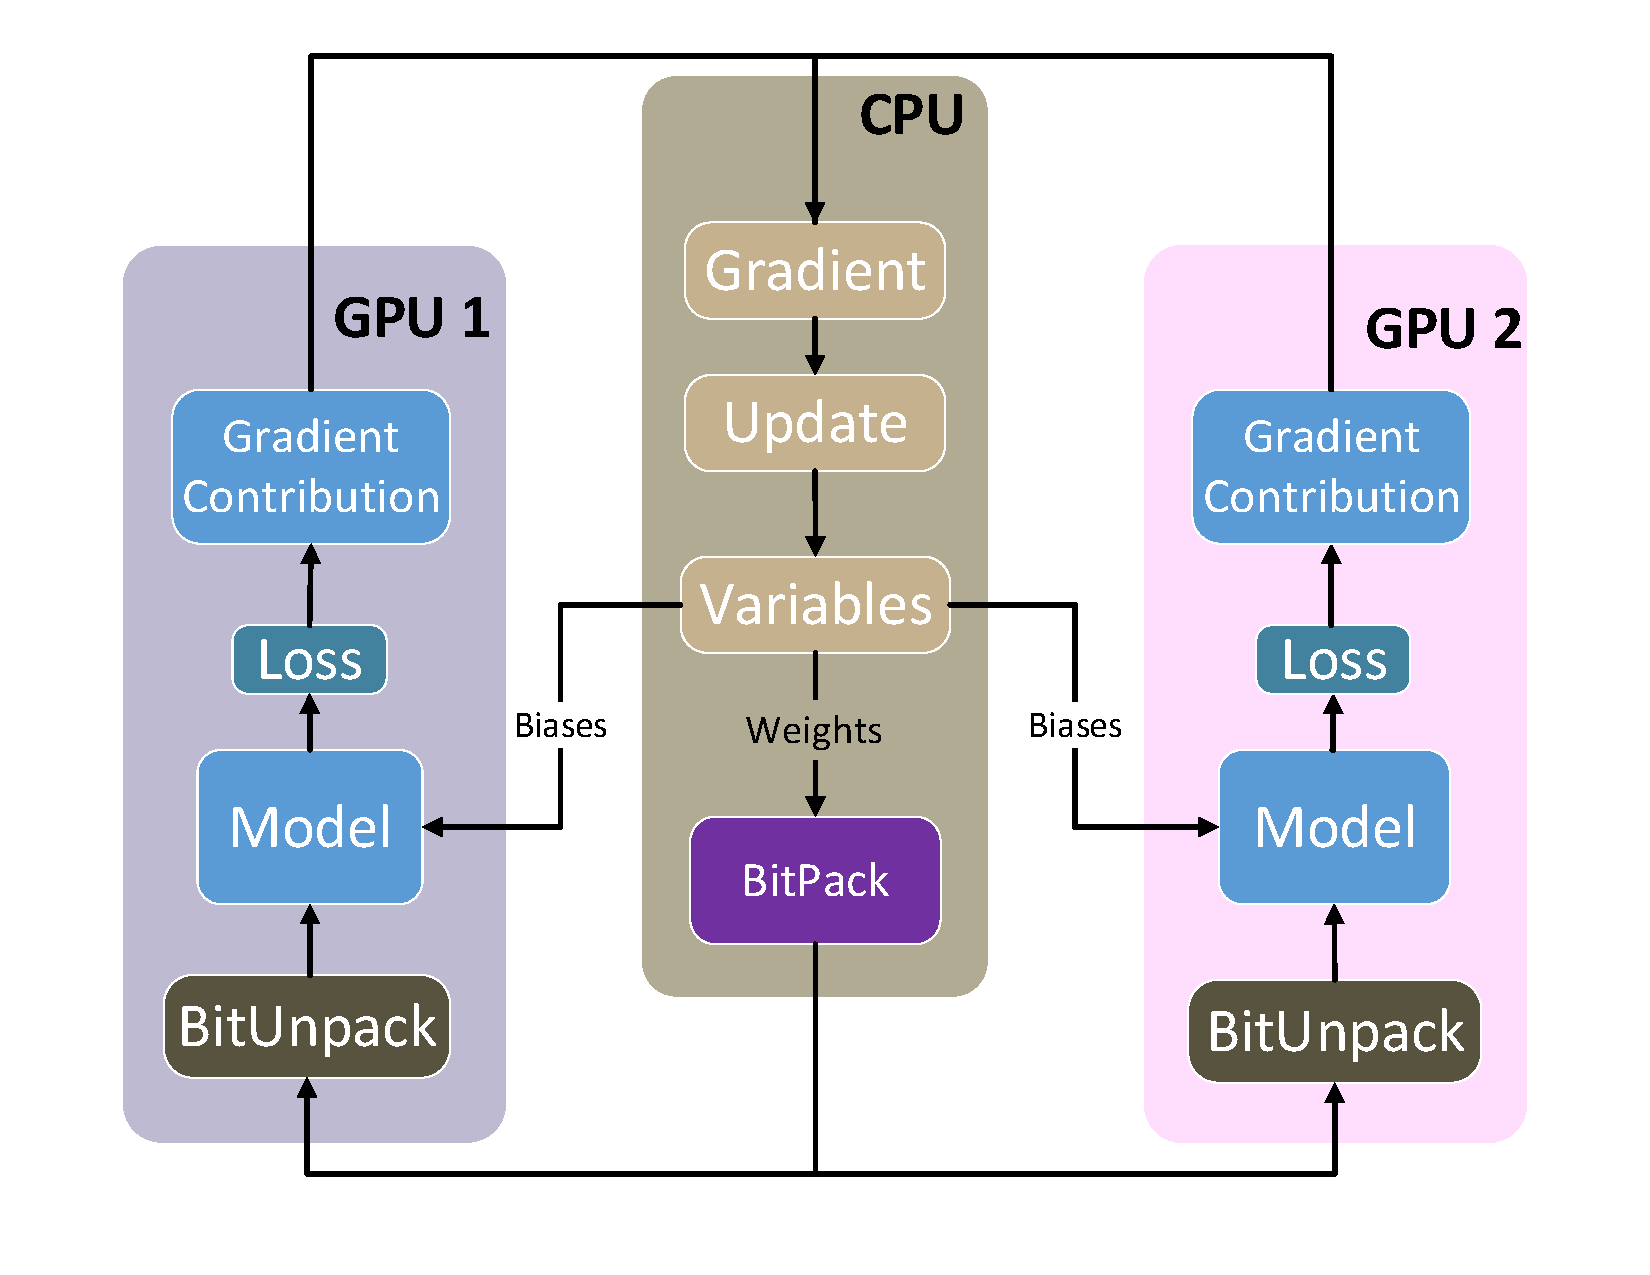
\includegraphics[scale=0.50]{bitpack/figs/drawing6.pdf}}
    %\centerline{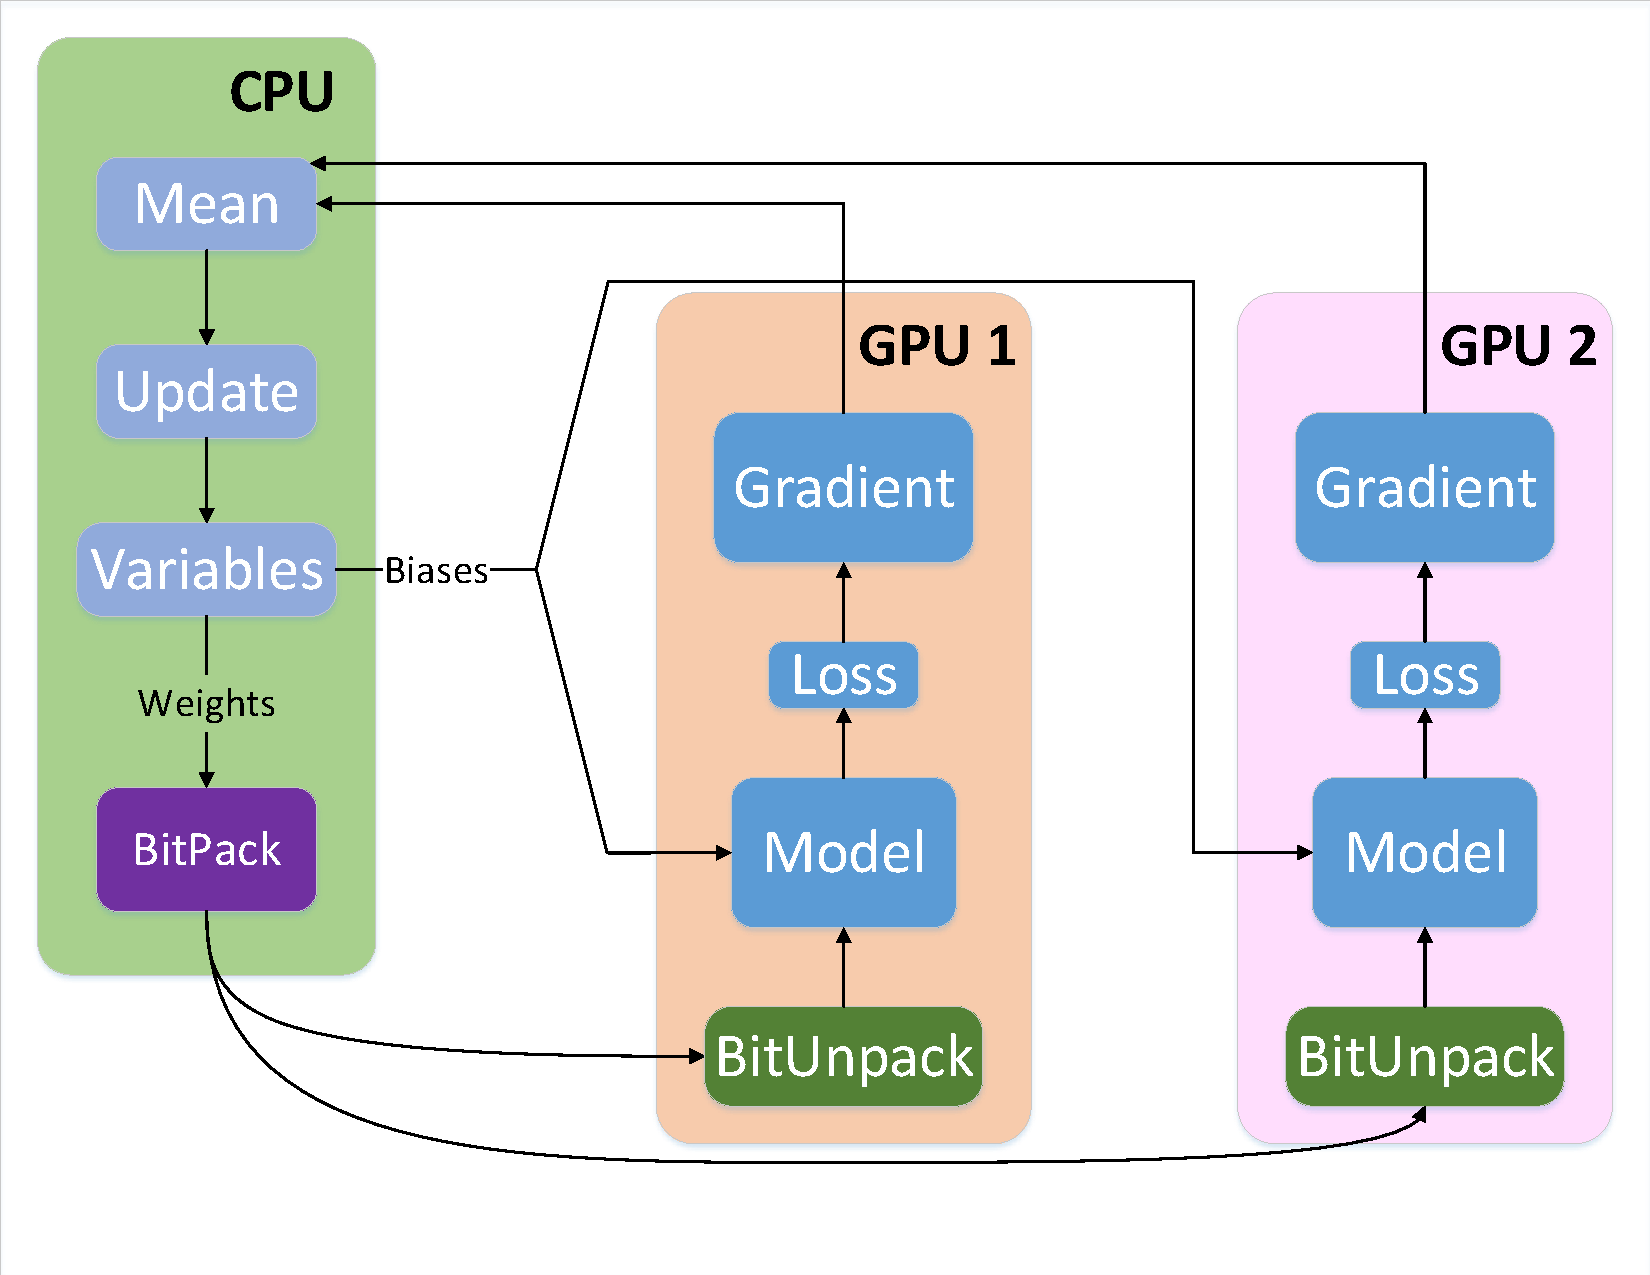
\includegraphics[scale=0.30]{bitpack/figs/tensorflow_multigpu.pdf}}
        \caption{The ADt on a 2-GPU system. Variables include: weights which go through
    the ADt procedure and biases which are sent directly to the GPUs to build the
    network model together with the unpacked weights.}
        \label{bitpack_mgpu}
\end{figure}

The Bitpack operation runs on CPU multicore devices.
To boost Bitpack  
we use OpenMP~\cite{openmp} and 
Single-Instruction Multiple Data (SIMD) intrinsics.
OpenMP is used to run Bitpack on several threads.
The use of SIMD instructions allows Bitpack to operate at the SIMD register level, which
avoids incurring large performance penalties in the process of producing the reduced-size weights.
We implement two versions of Bitpack.
One version uses Intel's AVX2~\cite{avx} instruction set and the other one relies on AltiVec~\cite{Altivec}. 
Bitpack can be implemented on top of any SIMD instruction set architecture supporting simple byte shuffling instructions at the register level.
The Bitunpack procedure runs on the GPUs.

It can be trivially parallelized since each weight is mapped
to a single 32-bit FP variable, which means that GPUs can process a
large amount of weights simultaneously and efficiently build the DNN model.
In fact, Bitunpack incurs negligible overhead as Section~\ref{sec:bitpack_performance} shows.

ADT manipulates the internal representation of network weights by discarding some bits.
We use the standard 32-bit IEEE-754 single-precision Floating Point format
~\cite{ieee754} (1 bit sign, 8 bits exponent and 23 bits mantissa) for all the computation routines.
The Bitpack method considers network weights as 32-bit 
words where rounding to $N$ bits means discarding the lowest $32-N$ bits.

\begin{algorithm}%[H]%algorithm* occupies full page
\caption{High Level Pseudo-code Version of Bitpack}
\label{alg:bitpack_na\"{i}ve}
{\fontsize{11}{11}\selectfont
\begin{algorithmic}[1]
    \State W
    \Comment Array of 32-bit Floating Point values containing weights
    \State Pw
    \Comment Array containing the reduced precision weights
    \State RoundTo
    \Comment Number of bytes to keep per weight
    \State POffset := 0
    \Comment Indicates the current size (in bytes) of Pw
    \For {weight \textbf{in} W}
        \State Pw[POffset : POffset+RoundTo] := weight[0 : RoundTo]
        \Comment Copy most significant RoundTo bytes to Pw
        \State POffset := POffset + RoundTo
    \EndFor
\end{algorithmic}
}
\end{algorithm}


\subsection{Bitpack}
\label{subsec:bitpack}
A high-level version of the Bitpack procedure in terms of pseudo-code is illustrated by 
Algorithm~\ref{alg:bitpack_na\"{i}ve}.
The algorithm requires a couple of arrays: the input array $W$, which contains all the weights of a certain network layer, and an 
output array $Pw$, which stores the compressed versions of these weights. 
The algorithm goes through 
the entire $W$ input array, per each weight, copies the most 
significant $RoundTo$ bytes to the output array $Pw$.
Our Bitpack implementation manipulates data at the byte granularity.
We do not observe significant performance benefits when operating at finer granularity in the experiments we run.
The AWP algorithm described in Section~\ref{sec:bitpack_adaptive} determines the data representation format per each network layer.  
The number of bits of the chosen format is rounded to the nearest number of bytes
that retains all of its information (E.g., if AWP provides the value 14, $RoundTo$ will be set to 2 bytes).
The $Pw$ array is sent to the GPUs once the Bitpack procedure finishes compressing network weights.
%Currently, the host (CPU) and device (GPU) transfer byte stream so a packing
%algorithm with a granularity beyond one byte (8-bit) incurs more complexity and
%has little impact on the communication footprint. Hence, all the bitpack
%algorithm variants we are going to introduce below have a granularity of one byte.

Deep networks usually contain tens or even hundreds of millions of 
weights~\cite{alexnet, alexnet2, vgg}, which makes any trivial implementation 
of Algorithm~\ref{alg:bitpack_na\"{i}ve} not applicable in practice.
We mitigate compression costs by observing that Algorithm~\ref{alg:bitpack_na\"{i}ve} is trivially parallel since processing one weight just requires the $RoundTo$ parameter.
Algorithm~\ref{alg:bitpack_omp} shows how to parallelize the Bitpack procedure by using OpenMP threads.
Each thread takes care of a certain portion of the array storing network weights.

\begin{algorithm}%[H]%algorithm* occupies full page
\caption{Bitpack with OpenMP}
\label{alg:bitpack_omp}
{\fontsize{11}{11}\selectfont
\begin{algorithmic}[1]
    \State W 
    \Comment Array of 32-bit Floating Point values containing weights
    \State Pw
    \Comment Array containing the reduced precision weights
    \State RoundTo 
    \Comment Number of bytes to keep per weight 
    \State NumThreads
    \Comment Number of OpenMP threads
    \State \textcolor{orange} {\#pragma omp parallel for} %public(Weights, Pweights, RoundTo, workload) 
%    \Comment Distribute a portion of weights W and Pw across OpenMP processes
      \For {weight \textbf{in} W}
            \State POffset := Corresponding position in Pw
            \State Pw[POffset : POffset+RoundTo] := weight[0 : RoundTo]
            \Comment Copy the most significant RoundTo bytes to Pw
      \EndFor
\end{algorithmic}
}
\end{algorithm}

\subsection{Single Instruction Multiple Data Bitpack}
Since all weights within one layer are processed in the same way by the Bitpack procedure, we can leverage Single Instruction Multiple Data (SIMD) instructions to vectorize it.
Most state-of-the-art architectures implement SIMD instruction set: IBM's 
AltiVec~\cite{Altivec}, Intel's Advanced Vector Extensions (AVX)~\cite{avx}, and ARM's Neon~\cite{neon}.
In our experiments we use
Intel's AVX2~\cite{avx}, which implements a set of SIMD 
instructions operating over 256-bit registers, and IBM's AltiVec instruction 
set~\cite{Altivec}, which has SIMD instructions operating over 128-bit registers.
Section~\ref{sec:bitpack_setup} describes the specific details of our evaluation considering both x86 and POWER architectures.
%There are also a set of intrinsic C/C++ that expose the AVX2 instructions to the software stack.  
%Intel provides a set of intrinsics for programming using the 
%SIMD instructions in C/C++, we henceforth will refer to the intrinsics rather than the 
%actual instructions.

Figure~\ref{bitpack_avx2} shows the byte-level operations of SIMD-based Bitpack applied to eight 32-bit weights and implemented with AVX2. 
The \textit{RoundTo} parameter is set to 3, which implies discarding the last 8 bits of 
each weight since the target data representation is 24-bit long. 
First, eight 32-bit Floating Point weights are loaded to a 256-bit register.
%of the 16 
%256-bit AVX2 registers. 
In the next step, we use \textit{\_mm256\_shuffle\_epi8} to shuffle the least significant
eight bits of each weight to the least significant bits of their respective 128-bit lane 
(see the grey area of Figure~\ref{bitpack_avx2} Step 2) and pack the rest of the bits 
together. 
Afterwards we use \textit{\_mm256\_permutevar8x32\_epi32} to do the same operation 
across the two 128-bit lanes. 
Finally, we use \textit{\_mm256\_maskstore\_epi32} to just store  
the resulting 192 bits to the target array.
Not all AVX2 instructions operate over the entire 256-bit register.
Instead, many of
them conceive the register as two 128-bit lanes and operate on them separately.
This is the reason way we can not carry out Steps 2 and 3 by using a single AVX2 instruction.


\definecolor{lightgray}{gray}{0.5}
\begin{figure}[H]%[bhtp]
    \centering
    \begin{bytefield}[bitwidth=1.15em, bitformatting={\tiny},endianness=big]{32}
        \wordbox{2}{\textit{\fontsize{11}{11} \selectfont 
            Step 1: Load 8 32-bit weights into a 256-bit AVX2 register. 
            \textcolor{cyan}{(\_mm256\_loadu\_si256)}}} \\ 
        \bitboxes{4}{{\tiny $H_{3..0}$}&{\tiny $G_{3..0}$}&{\tiny $F_{3..0}$}&
                    {\tiny $E_{3..0}$}&{\tiny $D_{3..0}$}&
                    {\tiny $C_{3..0}$}&{\tiny $B_{3..0}$}&{\tiny $A_{3..0}$}} \\
        \bitheader{0,3,7,11,15,19,23,27,31} \\
        \wordbox{2}{\textit{\fontsize{11}{11} \selectfont
            Step 2: Pack weights on the 2 128-bit lanes.
            \textcolor{cyan}{(\_mm256\_shuffle\_epi8)}}} \\
        \bitboxes{3}{{\tiny $H_{3..1}$}} & 
        \bitboxes{3}{{\tiny $G_{3..1}$}} & 
        \bitboxes{3}{{\tiny $F_{3..1}$}} & 
        \bitboxes{3}{{\tiny $E_{3..1}$}} & 
        \bitbox{4}{\color{lightgray}\rule{\width}{\height}} &
        \bitboxes{3}{{\tiny $D_{3..1}$}} &
        \bitboxes{3}{{\tiny $C_{3..1}$}} &
        \bitboxes{3}{{\tiny $B_{3..1}$}} &
        \bitboxes{3}{{\tiny $A_{3..1}$}} &
        \bitbox{4}{\color{lightgray}\rule{\width}{\height}} \\
        \bitheader{0,3,6,9,12,15,19,22,25,28,31} \\
        \wordbox{2}{\textit{\fontsize{11}{11} \selectfont
            Step 3: Pack the 8 weights together by rearranging 32-bit across 
            128-lanes.
            \textcolor{cyan}{(\_mm256\_permutevar8x32\_epi32)}}} \\
        \bitboxes{3}{{\tiny $H_{3..1}$}} & 
        \bitboxes{3}{{\tiny $G_{3..1}$}} & 
        \bitboxes{3}{{\tiny $F_{3..1}$}} & 
        \bitboxes{3}{{\tiny $E_{3..1}$}} & 
        \bitboxes{3}{{\tiny $D_{3..1}$}} &
        \bitboxes{3}{{\tiny $C_{3..1}$}} &
        \bitboxes{3}{{\tiny $B_{3..1}$}} &
        \bitboxes{3}{{\tiny $A_{3..1}$}} &
        \bitbox{8}{\color{lightgray}\rule{\width}{\height}} \\
        \bitheader{0, 7, 10, 13, 16, 19, 22, 25, 28, 31} \\
        \wordbox{2}{\textit{\fontsize{11}{11} \selectfont
            Step 4: Store the most significant 24 bytes (192 bits) of data into 
            the target array. \textcolor{cyan}{(\_mm256\_maskstore\_epi32)}}} \\
    \end{bytefield}
	\vspace{-0.5cm}
	\caption{Bitpack implemented with AVX2, RoundTo=3}
	\label{bitpack_avx2}
\end{figure}

%Algorithm~\ref{alg:bitpack_omp_avx} summarizes our implementation of the Bitpack procedure with AVX2.
%It exploits two-level parallelism: first, the input array of weights is distributed across several threads.
%Second, within each thread, the compression of each eight 32-bit weights subset is performed at the register level by means of byte shuffling instructions.  
%This sophisticated procedure exploiting parallelism at both thread and SIMD register levels uses all the available hardware at the multicore level and avoids costly memory accesses.

\begin{algorithm}%[H]%algorithm* occupies full page
\caption{Bitpack with OpenMP + AVX2}
\label{alg:bitpack_omp_avx}
{\fontsize{11}{11}\selectfont
\begin{algorithmic}[1]
    \State W
    \Comment Array of 32-bit Floating Point values containing weights
    \State Pw
    \Comment Array containing the reduced precision weights
    \State RoundTo
    \Comment Number of bytes to keep per weight
    \State \textcolor{orange} {\#pragma omp parallel for} %public(Weights, Pweights, RoundTo, workload) 
%    \For {process := 0 \ldots NumProcesses}
%        \State Distribute a portion of weights W and Pw across OpenMP processes
    \For {weights \textbf{in} W}
        \State \textcolor{cyan}{\_mm256\_loadu\_si256}
        \Comment Load 8 32-bit weights 
        \State \textcolor{cyan}{\_mm256\_shuffle\_epi8}
        \Comment Compress at each 128-bit lane
        \State \textcolor{cyan}{\_mm256\_permutevar8x32\_epi32}
        \Comment Shuffle the compressed weights into the most significant bits
        \State \textcolor{cyan}{\_mm256\_maskstore\_epi32}
        \Comment Store compressed weights to the target array
    \EndFor
\end{algorithmic}
}
\end{algorithm}

\begin{algorithm}%[H]%algorithm* occupies full page
\caption{Bitunpack on GPU}
\label{alg:bitunpack}
{\fontsize{11}{11}\selectfont
\begin{algorithmic}[1]
    \State Pw
    \Comment Array containing compressed weights
    \State W
    \Comment Array of 32-bit Floating Point values containing weights
    \State RoundTo
    \Comment The number of bytes that are going to be kept
    \For{UnitId := 0 \ldots NumUnit}
    \State Distribute W and Pw across all the computation units in the GPU
        \State POffset := 0
        \For{weight in W}
            \State weight := Pw[POffset : POffset+RoundTo] $\ll$ (4 - RoundTo) * 8
            \State POffset := POffset + RoundTo
        \EndFor
    \EndFor
\end{algorithmic}
}
\end{algorithm}

Algorithm~\ref{alg:bitpack_omp_avx} summarizes our implementation of the Bitpack procedure with AVX2.
It exploits two-level parallelism: first, the input array of weights is distributed across several threads.
Second, within each thread, the compression of each eight 32-bit weights subset is performed at the register level by means of byte shuffling instructions.
This sophisticated procedure exploiting parallelism at both thread and SIMD register levels uses all the available hardware and avoids costly memory accesses.

\subsection{Bitunpack}
Once data in reduced-size format reaches the target GPU, the Bitunpack procedure immediately 
restores them into their original IEEE-754 32-bit Floating Point format. 
We display pseudo-code describing this process in Algorithm~\ref{alg:bitunpack}.
Bitunpack reads the reduced-sized weights from array $Pw$ and assigns additional bits to them. 
Bitunpack gives zero values to these additional bits.
We distribute the Bitunpack process across the whole GPU, which enables an extremely parallel scheme exploiting GPUs manycore architecture. 

The Bitunpack routine is developed using CUDA~\cite{cuda}. 
Our code  
runs in parallel on $N$ CUDA threads and the CUDA runtime handles the dynamic mapping between threads and the underlying GPU compute units.
Since each thread involved in the parallel run targets a different portion of the $Pw$ array, our Bitunpack procedure exposes a large amount of parallelism able to exploit the large number of compute units integrated into high-end GPU devices.


\section{Experimental Setup}
\label{sec:bitpack_setup}
The experimental setup considers a large image dataset, three state-of-the-art 
neural network models and two high-end platforms.
The following sections describe all theses elements in detail.

\subsection{Image Dataset}
We consider the ImageNet ILSVRC-2012 dataset~\cite{imagenet}.
The original ImageNet dataset includes three sets of images of 1000 classes 
each:
training set (1.3 million images), validation set (50,000 images) and
testing set (100,000 images).
Considering 1000 classes makes the training process around 170 hours long, which 
is prohibitively expensive since our large experimental campaign considers 
different network models, batch sizes and hardware platforms.
To reduce the execution time of our experiments we consider a subset of 200 
classes for both the training and the validation dataset, which keeps the 
training time under manageable margins.
%  To speedup our experiments without hampering
%the quality of the results, we select a same set of 200 classes for both the
%training set and the validation set as our dataset.
For the rest of this paper, we refer to the 200 classes dataset as ImageNet200.
Since it is a common practice~\cite{vgg}, we evaluate the ability of a certain 
network in properly dealing with the ImageNet200 dataset in terms of the top-5 
validation error computed over the validation set.

\subsection{DNN Models and Training Parameters}
We apply the AWP algorithm along with the ADT procedure on three 
state-of-the-art DNN models: a modified version of Alexnet~\cite{alexnet} with 
an extra fully-connected layer of size 4096, the configuration A of the VGG 
model~\cite{vgg} and the Resnet network~\cite{resnet}.  All hidden layers are 
equipped with a Rectified Linear Units (ReLU)~\cite{alexnet}.
The exact configurations of the three neural networks are shown in 
Table~\ref{table:bitpack_config}.  The Alexnet model is composed of 5 convolutional 
layers and 4 fully-connected ones, VGG contains 8 convolutional layers and 3 
fully-connected ones and Resnet is composed of 33 convolutional layers and a 
single fully-connected one.

% Please add the following required packages to your document preamble:
% \usepackage{multirow}
\begin{table}[]
\caption{Neural network configurations: The convolutional layer parameters are 
    denoted as ``conv<receptive field size>-<number of channels>''. The ReLU 
    activation function is not shown for brevity. The building blocks of Resnet
    and the number of times they are applied are shown in a single cell.}
    \centering
    \begin{tabular}{|P{3.5cm}|P{3.5cm}|P{3.5cm}|}
\hline
    \textbf{Alexnet} & \textbf{VGG}  & \textbf{Resnet-34}  \\ \hline
\multicolumn{3}{|c|}{input(224x224 RGB image)}                                                                                                                                                 
        \\ \hline
conv11-64                                                  & conv3-64                                                      
        & conv7-64                                                           \\ 
        \hline
\multicolumn{3}{|c|}{maxpool}                                                                                                                                                                  
        \\ \hline
conv5-192                                                 & conv3-128                                                     
        & \begin{tabular}[c]{@{}c@{}}conv3-64\\ conv3-64\\ x3\end{tabular}   \\ 
            \hline
\multicolumn{2}{|c|}{maxpool}                                                                                             
        &                                                                    \\ 
        \hline
conv3-384                                                 & 
        \begin{tabular}[c]{@{}c@{}}conv3-256\\ conv3-256\end{tabular} & 
            \begin{tabular}[c]{@{}c@{}}conv3-128\\ conv3-128\\ x4\end{tabular} 
                \\ \hline
\multicolumn{2}{|c|}{maxpool}                                                                                             
        &                                                                    \\ 
        \hline
conv3-384                                                  & 
        \begin{tabular}[c]{@{}c@{}}conv3-512\\ conv3-512\end{tabular} & 
            \begin{tabular}[c]{@{}c@{}}conv3-256\\ conv3-256\\ x6\end{tabular} 
                \\ \hline
\multicolumn{2}{|c|}{maxpool}                                                                                             
        &                                                                    \\ 
        \hline
conv3-256                                                 & 
        \begin{tabular}[c]{@{}c@{}}conv3-512\\ conv3-512\end{tabular} & 
            \begin{tabular}[c]{@{}c@{}}conv3-512\\ conv3-512\\ x3\end{tabular} 
                \\ \hline
\multicolumn{2}{|c|}{maxpool}                                                                                             
        & avgpool                                                            \\ 
        \hline
\multicolumn{2}{|c|}{FC-4096}                                                                                             
        & \multicolumn{1}{l|}{\multirow{2}{*}{}}                             \\ 
        \cline{1-2}
\begin{tabular}[c]{@{}c@{}}FC-4096\\ FC-4096\end{tabular} & 
    \multicolumn{1}{c|}{FC-4096}                                  & 
        \multicolumn{1}{l|}{}                                              \\ 
        \hline
\multicolumn{3}{|c|}{FC-200}                                                                                                                                                                   
        \\ \hline
\multicolumn{3}{|c|}{softmax}                                                                                                                                                                  
        \\ \hline
\end{tabular}
\label{table:bitpack_config}
\end{table}

We use momentum SGD~\cite{momentum} to guide the training process with momentum 
set to 0.9.  The training process is regularized by weight decay and  the 
$L_{2}$ penalty multiplier is set to $5\times10^{-4}$.  We apply a dropout 
regularization value of 0.5 to fully-connected layers.
We initialize the weights using a zero-mean normal distribution with variance 
$10^{-2}$.  The biases are initialized to $0.1$ for Alexnet and $0$ for both VGG 
and Resnet networks.
For the Alexnet and VGG models we consider training batch sizes of 64, 32 and 
16.
To train the largest network we consider, Resnet, we consider batch sizes of 
128, 64 and 32.
The 16 batch size incurs in a prohibitively expensive training process for 
Resnet and, therefore, we do not use it in our experimental campaign. 
%
%There are several factors to take into consideration that affect the
%benefits provided by this papers' proposals.
%Among the most important ones we have the number of weights of the considered 
%neural network, which define the size of the data transfers over which our 
%solution is deployed, or the batch size, which defines the number of samples 
%each batch is composed of.  Since the network weights are updated every time a 
%batch is processed, the smaller the batch size is, the more frequent are the 
%weight updates and, thus, the larger is the potential of our solution for 
%improving performance.
%In order to cover these factors,
%we train both neural networks using a set of three batch sizes: 64, 32 and 16.
%

For Alexnet we set the initial learning rate to $10^{-2}$ for the 64 batch size 
and decrease it by factors of 2 and 4 for the 32 and 16 batch sizes, 
respectively.
In the case of VGG we set the initial learning rate to $10^{-2}$ for the 64, 32 
and 16 batch sizes, as in the state-of-the-art~\cite{vgg}.  In the case of 
Resnet the learning rate is $10^{-2}$ for the batch size of 32 and 0.1 for the 
rest.  For all network models we apply exponential decay to the learning rate 
throughout the whole training process in a way the learning rate decays every 30 
batches by a factor of 0.16, as previous work suggests~\cite{alexnet2}.
For Resnet we obtain better results by adapting precision at the Resnet building 
blocks level~\cite{resnet} instead of doing so in a per-layer basis.
%\textcolor{cyan}{Our preliminary experiments suggest that by applying our 
%approach to all of the layers separately on Resnet does not provide any 
%benefit. Instead, we group the layer in terms of the resnet building 
%blocks~\cite{resnet} and apply our approach on that level.}

\subsection{Implementation}
Our code is written in Python on top of Google Tensorflow~\cite{tensorflow}.
Tensorflow is a data-flow and graph-based numerical library where the actual 
computation is carried out according to a computational graph constructed 
beforehand.
The computational graph defines the order and the type of computations that are 
going to take place. It supports NVIDIA's NCCL library.

To enable the use of both Bitpack and Bitunpack routines, we integrate them into 
Tensorflow using its C++ API.
Tensorflow executes the two routines before sending the weights from the CPU to 
the GPU and right after receiving the weights on the GPU side, respectively.
The Bitpack routine is implemented using the OpenMP 4.0 programming model.  
There are two versions of this routine using either Intel's AVX2 or AltiVec 
instructions, as explained in Section~\ref{sec:bitpack_approx}.
Bitunpack is implemented using CUDA 8.0 and CUDA 10.0 respectively on the two 
platforms~\cite{cuda}.

\subsection{Hardware Platforms}
\label{sec:platform}
We conduct our experiments on two clusters featuring the x86 and POWER 
architectures.
The x86 machine is composed of two 8-core Intel Xeon
\textregistered E5-2630 v3 (Haswell) at 2.4 GHz and a 20 MB L3 shared cache 
memory each.  It is also equipped with two Nvidia Tesla K80 accelerators, each 
of which hosts two Tesla GK210 GPUs.
It has 128 GB of main memory, distributed in 8 DIMMs of 16 GB DDR4 @ 2133 MHz.
The 16-core CPU and the four GPUs are connected via a PCIe 3.0 x8 8GT/s.
The operating system is RedHat Linux 6.7.
Overall, the peak performance of the two 8-core sockets plus the four Tesla 
GK210 GPUs is 6.44 TFlop/s.

The POWER machine is composed of two 20-core IBM POWER9 8335-GTG at 3.00 GHz.  
It contains four NVIDIA Volta V100 GPUs.  Each node has 512 GB of main memory, 
distributed in 16 DIMMS of 32 GB @ 2666 MHz.
The GPUs are connected to the CPU devices via a NVIDIA NVLink 2.0 
interconnection~\cite{nvlink}.
The operating system is RedHat Linux 7.4.
The peak performance of the two 20-core sockets plus the four V100 GPUs is 28.85 
TFlop/s.

\section{Evalutation}
\label{sec:bitpack_evaluation}
In this section we evaluate the capacity of the AWP algorithm and the ADT procedure to accelerate DNNs training. 
We show how our proposals are able to accelerate the training phase of relevant DNN models without reducing the accuracy of the network. 

\subsection{Methodology}
\label{sec:evaluation1}

\begin{figure*}[!bhtp]
    \hbox{%\hspace{7.0mm}
        \centerline{
            \includegraphics[scale=0.450]{bitpack/figs/vgg/small_3/vgg_validation_top5_64-$A^2$DtWp.pdf}
            \includegraphics[scale=0.450]{bitpack/figs/vgg/small_3/vgg_validation_top5_32-$A^2$DtWp.pdf}
        }
    }
    \hbox{%\hspace{7.0mm}
        \centerline{
            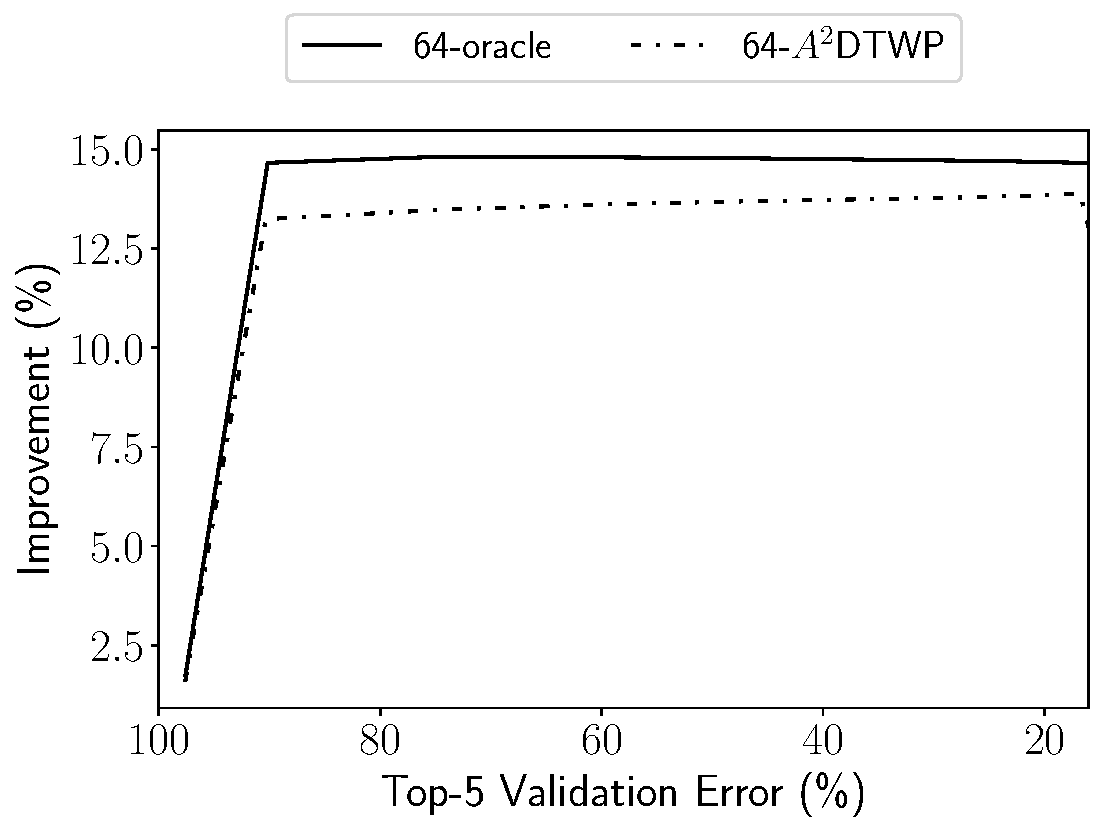
\includegraphics[scale=0.450]{bitpack/figs/vgg/small_3/vgg_train_improvement_agg_top5_64-baseline.pdf}
            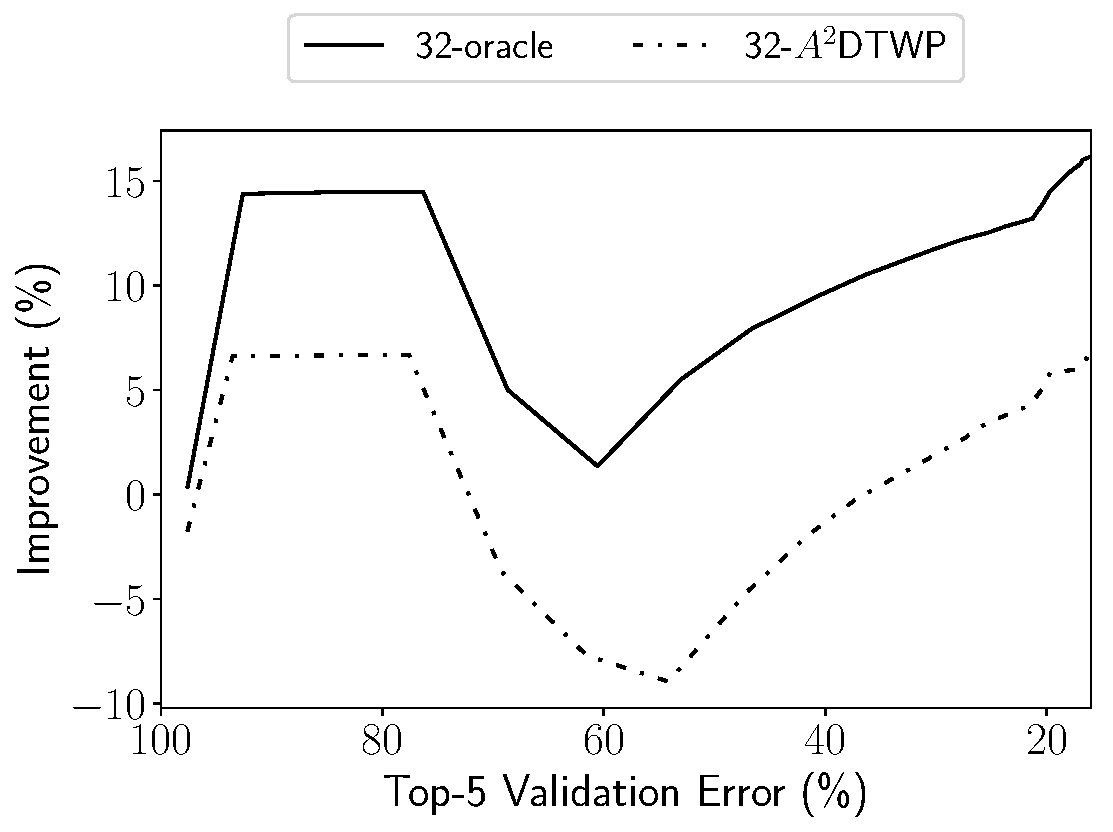
\includegraphics[scale=0.450]{bitpack/figs/vgg/small_3/vgg_train_improvement_agg_top5_32-baseline.pdf}
        }
    }
    \caption{VGG training considering 64 and 32 batch sizes. The 
    two upper plots show the top-5 validation error evolution of
    \textit{baseline}, \textit{oracle} and \textit{$A^2$DTWP}.
    The two bottom figures provide information on the performance improvement of
    \textit{oracle} and \textit{$A^2$DTWP} against \textit{baseline} during the
    training process. Experiments run on the x86 system.
    %\rephrased{Figures upgraded from using continuous lines to using points}
    }
    \label{vgg_improv}
    %\vspace{-0.5cm}
\end{figure*}

%We conduct a set of experiments on several batch sizes (16, 32, 64) for both Alexnet and VGG. 
Our experimental campaign considers batch sizes of 64, 32 and 16 for the Alexnet and VGG models and 128, 64 and 32 for the Resnet network.
For each model and batch size, the \emph{baseline} run uses the 32-bit Floating Point precision for the whole training. 
The data represention formats we consider to transfer weights from the CPU to the GPU are:
8-bit (1 bit for sign, 7 bits for exponent), 16-bit (1 bit for sign, 8 for exponent, 7 for mantissa), 24-bit (1 bit for sign, 8-bits for exponent and 15 bits for mantissa) and 32-bits (1 bit for sign, 8 bits for exponent and 23 bits for mantissa).
We train the network models with dynamic data representation by applying the AWP algorithm along with the ADT procedure.
We denote this approach combining ADT and AWP as \textit{$A^2$DTWP}.  
For each DNN and batch size, we select the data representation format that first 
reaches the 35\%, 25\% and 15\% accuracy thresholds for Resnet, Alexnet and VGG, respectively, and we 
denote this approach as \emph{oracle}.
For the case of the \emph{oracle} approach, data compression is done via ADT.
The closer \textit{$A^2$DTWP} is to \emph{oracle}, the better is the AWP algorithm in identifying the best data representation format.

During training we sample data in terms of elapse time and validation error every 4000 batches. 
The total number of training batches corresponding to the whole ImageNet200 dataset are 16020, 8010, 4005 and 2002 for batch sizes 16, 32, 64 and 128, respectively.
The values of $AWP$ parameters $T$, $INTERVAL$, and $N$ are determined in the following way:
In the case of $T$ we monitor the execution of several epochs until we observe a drop in the validation error. 
We then measure the average change, considering all layers, of weights' $l^2$-norm during this short monitoring period.
The obtained values of $T$ are $-5\times10^{-2}$, $-2\times10^{-3}$ and $-2\times10^{-5}$ for Alexnet, VGG and Resnet, respectively.
We set the $INTERVAL$ parameter to $4000$ for both AlexNet and VGG and $2000$ for Resnet. 
These values correspond to a single batch (for the ImageNet200 dataset and batch sizes 64 and 128) and avoid premature precision switching due to numerical fluctuations.  
We set $N$ to $8$ since the smallest granularity of our approach is 1 byte.
AWP initially applies 8-bit precision to all layers.
We use ImageNet200 in Sections~\ref{sec:alexnet}, ~\ref{sec:VGG}, ~\ref{sec:Resnet}, ~\ref{sec:Average}, and ~\ref{sec:performance}.
Section~\ref{sec:ImageNet1000} uses ImageNet1000.

\subsection{Evaluation on Alexnet}
\label{sec:alexnet}
The evaluation considering the Alexnet model on the x86 system is shown in  
Figure~\ref{alex_improv}, which plots detailed results considering batch sizes of 
32 and 16, and Figure~\ref{fig:all}, which shows the total execution time of the 
\textit{oracle} and \textit{$A^2$DTWP} policies normalized to the \textit{baseline} 
for the 64, 32 and 16 batch sizes on both the x86 and the POWER systems.
The two top plots of Figure~\ref{alex_improv} depict how the validation error of the 
\textit{baseline}, \textit{oracle}, and \textit{$A^2$DTWP} policies evolves 
over time for the 32 and the 16 batch sizes until the 25\% accuracy is reached.
The two bottom plots provide information regarding the performance 
improvement of both \textit{oracle} and \textit{$A^2$DTWP} over the 
32-bit \textit{baseline} with regard to a certain validation error. 
Such performance improvement is computed by looking at the time required by the 
\textit{oracle} and \textit{$A^2$DTWP} techniques to reach a certain validation error with respect to the \textit{baseline}.

It can be observed in the upper left-hand side plot of Figure~\ref{alex_improv} how 
the \textit{oracle} and the \textit{$A^2$DTWP} approaches are 10.82\% and 6.61\% faster than the baseline, respectively, to reach the 25\% top-5 validation error when using a 32 batch size.
The upper right-hand side plot shows results considering a 16 batch size. 
The improvements achieved by the 
\textit{oracle} and \textit{$A^2$DTWP} approaches are 11.52\% and 10.66\%, respectively.
This demonstrates 
the efficiency of the ADT procedure in compressing and decompressing the network weights without undermining the performance benefits obtained from sending less data
from the CPU device to the GPU.
It also demonstrates the capacity of AWP to quickly identify the best data representation format per layer.

The two bottom plots of Figure~\ref{alex_improv} provide information on 
performance improvement of \textit{oracle} and \textit{$A^2$DTWP} over the \textit{baseline} during the training process.
%One of the right-hand side plots of Figure~\ref{alex_improv} shows results when considering the 32 batch size.
For the 32 batch size, \textit{oracle} reaches a peak improvement of 24.11\% when the 90\%  
validation error is reached and steadily declines from that point although it keeps a significant 
improvement of 10.82\% over the \textit{baseline} once the 25\% top-5 validation error is reached. 
\textit{$A^2$DTWP} falls in-between the \textit{baseline} and the \textit{oracle}  
and keeps its improvement above 7.03\% until it reaches the 27\% top-5 validation error.
Once it reaches the 25\% validation error \textit{$A^2$DTWP} is 6.51\% faster than the \textit{baseline}.
In conclusion, the \textit{$A^2$DTWP} policy is able to provide performance 
improvements that are close to the ones achieved by the best possible accuracy.
%while the \textit{best} reaches 9.39\% at 25\% validation error.
For the 16 batch size, the performance benefits of the 
\textit{oracle} policy reach a 41.64\% peak at the 94\% validation error point.
The \textit{$A^2$DTWP} policy reaches its maximum performance benefit, 34.21\%, when the validation error is 97\%.
At the 25\% validation error point, the \textit{oracle} and the 
\textit{$A^2$DTWP} policies reach 13.00\% and 10.75\% performance improvement, respectively.
Overall, results considering the Alexnet network for batch sizes 
32 and 16 confirm that \textit{$A^2$DTWP}, which combines both the 
AWP algorithm and the ADT procedure, successfully delivers very similar 
performance benefits to the best possible accuracy.

Figure~\ref{fig:all} shows the normalized execution time of the \textit{oracle} 
and \textit{$A^2$DTWP} policies with respect to the 32-bit FP \textit{baseline} on the x86 and the POWER systems. 
The top chart reports performance improvements of 10.75\%, 6.51\%, and 0.59\% for batch sizes 16, 32 and 64 in
the case of Alexnet runnig on the x86 system.  
For the 64 batch size, the marginal gains of \textit{$A^2$DTWP} over the \textit{baseline} are due the poor performance of the 8-bits format employed by \textit{$A^2$DTWP} at the beginning of the training process.
This format does not contribute to reduce the validation error for the 64 batch case, which makes the \textit{$A^2$DTWP} policy to fall behind the \textit{baseline} at the very beginning of the training process.  
Although \textit{$A^2$DTWP} eventually increases its accuracy and surpases the \textit{baseline}, it does not provide the same significant performance gains for Alexnet as the ones observed for batch sizes 16 and 32.

\textit{$A^2$DTWP} performance improvements on the POWER system in the case of 
Alexnet are 18.61\%, 14.25\% and 10.01\% with respect to the \textit{baseline} for batch sizes 16, 32 and 64, respectively.  
The POWER system achieves larger performance improvements than x86 since the 
Bitpack procedure can be further parallelized over the 40 cores of the POWER9 
multicore chips than the 16 cores available in the Haswell multicore devices of the x86 system. 
This mitigates the costs of weigths' compression and thus provides larger performance improvements. 

\subsection{Evaluation on VGG}
\label{sec:VGG}

Figure~\ref{vgg_improv} shows results for batch sizes 64 and 32 when using the 
VGG architecture on the x86 system. 
The upper figures display the temporal evolution of the validation error until the 15\% top-5 validation error is reached.
Like in Alexnet, both the \textit{$A^2$DTWP} and the \textit{oracle} policies outperform the \textit{baseline}.
In the case of batch size 64, both \textit{oracle} and \textit{$A^2$DTWP} 
display a similar evolution in terms of validation error, which translates to 
very close performance improvement over the baseline. 
They maintain an overall improvement of over 13.00\% against the \textit{baseline} 
during most of their training. The \textit{$A^2$DTWP} technique outperforms the baseline by 
12.88\% when reaches 15\% of top-5 validation error while the 
\textit{oracle} policy achieves the same improvement.
For batch size 32 the final improvement achieved by \textit{$A^2$DTWP} over the baseline is 5.02\%.
This improvement is not as large as the one achived for the 64 batch size since the AWP algorithm does not identify a numerical precision able to beat the \textit{baseline} until the 57\% validation error is reached, as it can be seen in the bottom right hand side plot of Figure~\ref{vgg_improv}. 
%Despite this issue, \textit{$A^2$DTWP} still achieves a remarkable performance improvement of {\bf XX\%} over the baseline.

Figure~\ref{fig:all} shows the normalized execution time of \textit{$A^2$DTWP} 
and \textit{oracle} with respect to the \textit{baseline} for VGG considering 
batch sizes of 16, 32 and 64 on the x86 and POWER systems.
When applied to the VGG model on the x86 system, \textit{$A^2$DTWP} outperforms the 32-bit Floating Point \textit{baseline} by 12.88\%, 5.02\% and 7.31\% for batch sizes 64, 32 and 16, respectively.
Despite the already described issues suffered by the \textit{$A^2$DTWP} technique when applied to the 32 batch size, this approach achieves very remarkable performance improvements over the baseline in all considered scenarios. 

The performance improvements observed when trying VGG on the POWER system are even higher.
\textit{$A^2$DTWP} outperforms the \textit{baseline} by 28.21\%, 20.19\% and 11.13\% when using the 16, 32 and 64 batch sizes, respectively.
The performance improvement achieved on the POWER system are larger than the ones observed for x86 since the Bitpack procedure can be parallelized over 40 cores when running on the POWER system.
We observe the same behavior for Alexnet, as Section~\ref{sec:alexnet} indicates.

\subsection{Evaluation on Resnet}
\label{sec:Resnet}
We display the normalized execution time of the \textit{$A^2$DTWP} and the \textit{oracle} policies when applied to the Resnet model using batch sizes of 128, 64 and 32 in Figure~\ref{fig:all}.
In the case of Resnet we do not show detailed plots describing the evolution of 
the validation error during training because its behavior is very close to some previously displayed scenarios like VGG.
On the x86 system, \textit{$A^2$DTWP} beats the 32-bit Floating Point baseline by 4.94\%, 4.39\% and 3.11\% for batch sizes of 128, 64 and 32, respectively, once a top-5 validation error of 30\% is reached.
The relatively low performance improvement achieved in the case of 32 batch size is due to a late identification of a competitive numerical precision, as it happens in the case of VGG and batch size 32.

The performance gains on the POWER system display a similar trend as the ones achieved on x86. 
While they show the same low improvement for the 32 batch size, 2.12\%, \textit{$A^2$DTWP} achieves 6.92\% and 11.54\% performance gains for batch sizes 64 and 128, respectively.
\textit{$A^2$DTWP} achieves the largest performance improvement with respect to the 32-bit \textit{baseline} when run on the POWER system due to the reasons described in Sections~\ref{sec:alexnet} and~\ref{sec:VGG}.

\subsection{Average Performance Improvement}
\label{sec:Average}
The average performance improvement of \textit{$A^2$DTWP} over the 
\textit{baseline} considering the Alexnet, VGG and Resnet models reach 6.18\% and 11.91\% on the x86 and the POWER systems, respectively. 
As we explain in previous sections, \textit{$A^2$DTWP} obtains larger improvements on the POWER system than on  
x86 since the ADT procedure can be further parallelized over the 40 cores of the POWER9 multicore devices.
In contrast, the two Haswell devices of the x86 system offer just 16 cores for ADT.

The combination of the AWP algorithm and the ADT procedure properly adapts the precision of each network layer and compresses the corresponding weigths with a minimal overhead.
The large performance improvement obtained while training deep networks on two high-end computing systems demonstrate the effectiveness of \textit{$A^2$DTWP}.

\begin{figure*}%[!bhtp]
    \centerline{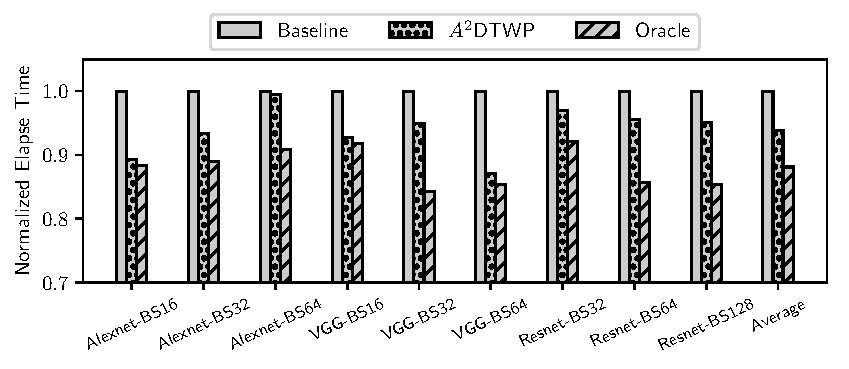
\includegraphics[scale=0.85]{bitpack/figs/all_bars.pdf}}
    %\vspace{-0.2cm}
    \centerline{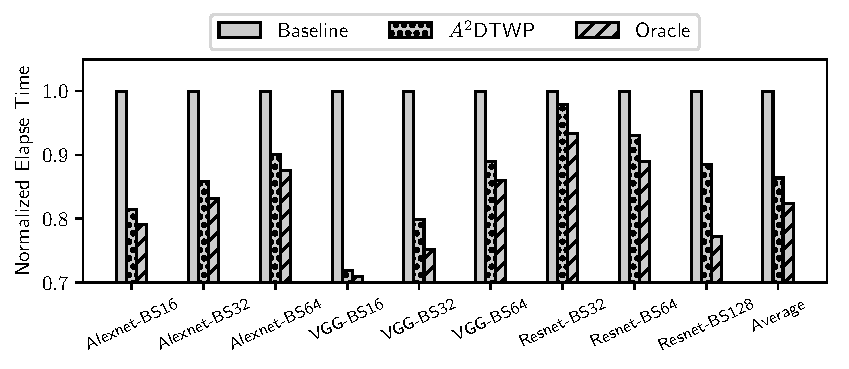
\includegraphics[scale=0.85]{bitpack/figs/all_bars_p9.pdf}}
    %\vspace{-0.5cm}
    \caption{Normalized execution times of the \textit{$A^2$DTWP} and the \textit{oracle} policies with respect to the baseline. 
Results obtained on the x86 system appear in the upper plot while the evalution on the POWER system appears at the bottom.} 
    \label{fig:all}
\end{figure*}

\subsection{$A^2DTWP$ Performance Profile}
\label{sec:performance}
This section provides a detailed performance profile describing the effects of 
applying $A^2DTWP$ when training the VGG network model with batch size 64 on the x86 and POWER systems described in section~\ref{sec:platform}.
To highlight these effects we also show a performance profile of applying 32-bit 
Floating Point format during training.
The main kernels involved in the training process and their corresponding average execution time in milliseconds are shown in Tables ~\ref{table:performance} and~\ref{table:performance_p9}.
Each kernel can be invoked multiple times by different network layers and it can be overlapped with other operations while processing a batch.
Tables~\ref{table:performance} and~\ref{table:performance_p9} display for all kernels the average execution time of their occurrences within a batch when run on the x96 and the POWER systems, respectively.

Results appearing in Table~\ref{table:performance} show how time spent transferring 
data from the CPU to the GPU accelerators when applying $A^2DTWP$ on the x86 system, 52.27 ms, 
is significantly smaller than the cost of performing the same operation when using the 32-bit configuration, 153.93 ms. 
This constitutes a 2.94x execution time reduction that compensates the cost of the operations involved in the ADT routine, Bitpack and
Bitunpack, and in the AWP algorithm, the $l^2$-norm computation.
On POWER we observe a similar reduction of 3.20x in the time spent transferring
data from the CPU to the GPUs when applying $A^2DTWP$.
These reductions in terms of CPU to GPU data transfer time are due to a close to 3x reduction in terms of weights size enabled by $A^2DTWP$.
The average execution time of operations where the $A^2DTWP$ technique plays no role remains very similar for the 32-bit Floating Point baseline and $A^2DTWP$ in both systems, as expected.
Tables~\ref{table:performance} and~\ref{table:performance_p9} indicate that performance gains achieved by $A^2DTWP$ are due to data motion reductions, which validates the usefulness of $A^2DTWP$.

Tables~\ref{table:performance} and~\ref{table:performance_p9} also display the overhead associated with AWP and ADT in terms of milliseconds.
The AWP algorithm spends most of its runtime computing the $l^2$-norm of the weights, which takes a total of 3.88 ms within a batch on the x86 system. 
On POWER, the cost of computing the $l^2$-norm of the weights is 0.93 ms.
The other operations carried out by AWP have a negligible overhead.
The two fundamental procedures of ADT are the Bitpack and Bitunpack routines, which take 19.71 and 4.51 ms to run within a single batch on the x86 system.
For the case of POWER, Bitpack and Bitunpack take 10.51 and 1.11 ms, respectively.
Overall, measurements displayed at Table~\ref{table:performance} indicate that AWP and ADT constitute 1.05\% and 6.60\% of the total batch execution time, respectively, on x86.
On the POWER system, AWP and ADT constitute 0.54\% and 6.82\% of the total batch execution time according to Table~\ref{table:performance_p9}. 
Figures ~\ref{alex_improv}, ~\ref{vgg_improv} and ~\ref{fig:all} account for this overhead in the results they display.

\begin{table}
    \caption{Performance profiles of both the $A^2DTWP$ and the 32-bit Floating 
    Point approaches expressed in milliseconds on the x86 system. 
    We consider the VGG network model with batch size 64.} 
    %\vspace{-0.35cm}
    \centering
    \begin{tabular}{|P{4.5cm}|P{2.5cm}|P{2.5cm}|}
    \hline
    %\rowcolor{LightCyan}
    & \textbf{32-bit FP} & $\mathbf{A^2DTWP}$\\
    \hline
    %\rowcolor{LightCyan}
    Data Transfer CPU$\rightarrow$GPU& 153.93 & 52.27 \\
    \hline
    %\rowcolor{LightCyan}
    Data Transfer GPU$\rightarrow$CPU& 68.51 & 73.55 \\
    \hline
    %\rowcolor{LightCyan}
    Convolution & 128.72 & 126.13\\
    \hline
    %\rowcolor{LightCyan}
    Fully-connected & 33.51 & 34.17 \\
    \hline
    %\rowcolor{LightCyan}
    Gradient update & 54.39 & 52.86\\
    \hline
    %\rowcolor{LightCyan}
    AWP ($l^2$-norm) & N/A & 3.88 \\
    \hline
    %\rowcolor{LightCyan}
    ADT (Bitpack) & N/A & 19.71 \\
    \hline
    %\rowcolor{LightCyan}
    ADT (Bitunpack) & N/A & 4.51 \\
    \hline
    \end{tabular}
    \label{table:performance}
\end{table}

\begin{table}
    \caption{Performance profiles of both the $A^2DTWP$ and the 32-bit Floating 
    Point approaches expressed in milliseconds on the POWER system. 
    We consider the VGG network model with batch size 64.} 
    %\vspace{-0.35cm}
    \centering
    \begin{tabular}{|P{4.5cm}|P{2.5cm}|P{2.5cm}|}
    \hline
    & \textbf{32-bit FP} & $\mathbf{A^2DTWP}$ \\
    \hline
    Data Transfer CPU$\rightarrow$GPU& 39.12 & 12.21 \\
    \hline
    Data Transfer GPU$\rightarrow$CPU& 17.34 & 17.87 \\
    \hline
    Convolution & 69.78 & 71.21\\
    \hline
    Fully-connected & 12.66 & 13.51 \\
    \hline
    Gradient update & 41.29 & 42.98\\
    \hline
    AWP ($l^2$-norm) & N/A & 0.93 \\
    \hline
    ADT (Bitpack) & N/A & 10.51 \\
    \hline
    ADT (Bitunpack) & N/A & 1.11 \\
    \hline
    \end{tabular}
    \label{table:performance_p9}
\end{table}

\subsection{Experiments with ImageNet1000}
\label{sec:ImageNet1000}
We run experiments considering ImageNet1000 to confirm they display the same trends as executions with ImageNet200. 
Network parameters are the same as the ones described in Section~\ref{sec:setup}.
$AWP$ parameters are the ones described in Section~\ref{sec:evaluation1}.
The experimental setup of the evaluation considering ImageNet1000 is the same as the one we use for ImageNet200.
We consider batch sizes that produce the fastest 32-bit FP training for each one of the network models: 64, 64, and 128 for Alexnet, VGG and Resnet, respectively.


Figure~\ref{fig:ImageNet1000} displays results corresponding to the experimental campaign with ImageNet1000 on the x86 system.
In the x-axis we display different epoch counts for each one of the three models: 4, 8, 12, 16, and 20 epochs for Alexnet; 2, 4, 6, and 8 for VGG; and 4, 8, 12, and 16 epochs for Resnet.
The y-axis displays the normalized elapsed time of \textit{$A^2$DTWP} with respect to the the 32-bit Floating Point \textit{baseline} per each model and epoch count.
For the case of Alexnet with batch size 64, \textit{$A^2$DTWP} is slightly faster than the \textit{baseline} as it displays a normalized execution time of 0.995, 0.992, 0.992, 0.996, and 0.990 after 4, 8, 12, 16 and 20 epochs, respectively.
Figure~\ref{fig:all} also reports small gains for the case of Alexnet with batch size 64, which confirms that experiments with ImageNet1000 show very similar trends as the evaluation with ImageNet200.
When applying \textit{$A^2$DTWP} to VGG with 64 batch size, it displays a normalized execution time of 0.907, 0.920, 0.936, and 0.932 with respect to the \textit{baseline} after running 2, 4, 6 and 8 training epochs, respectively.
For the Resnet example, we observe normalized execution times of 0.765, 0.770, 0.778, and 0.777 for \textit{$A^2$DTWP} after 4, 8, 12, and 16 training epochs, respectively,
which constitutes a significant performance improvement.

\begin{figure}%[!bhtp]
    \centerline{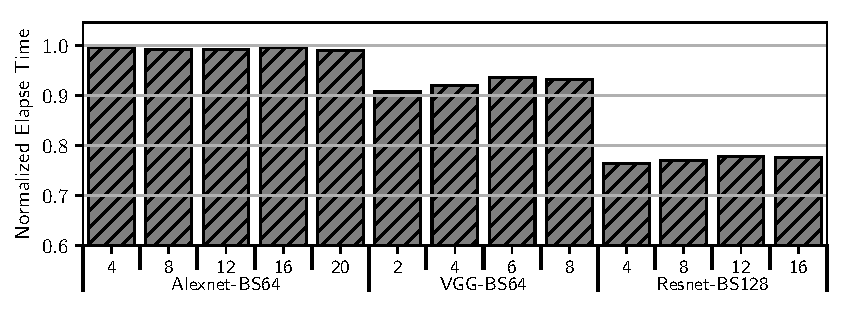
\includegraphics[scale=0.85]{bitpack/figs/imagenet-1k-3net.pdf}}
    \caption{Normalized execution time of \textit{$A^2$DTWP} with respect to \textit{baseline} considering the Imagenet1000 data set. Training for Alexnet, VGG and Resnet considers up to 20, 8, and 16 epochs, respectively.}
    \label{fig:ImageNet1000}
\end{figure}

In terms of validation error, both \textit{$A^2$DTWP} and \textit{baseline} display very similar top-5 values at the end of each epoch.
For example, for the case of VGG, the Floating Point 32-bit \textit{baseline} approach displays a validation error of 88.04\% after 2 training epochs while \textit{$A^2$DTWP} achieves a validation error of 89.97\% for the same epoch count, that is, an absolute difference of 1.93\%.
After 4, 6, and 8 training epochs absolute distances of top-5 validation errors between \textit{$A^2$DTWP} and \textit{baseline} are 3.09\%, 0.47\%, and 0.71\%, respectively.
Top-5 validation error keeps decreasing in an analogous way for both \textit{baseline} and \textit{$A^2$DTWP} as training goes over more epochs, although \textit{$A^2$DTWP} is significantly faster.
Our evaluation indicates that \textit{$A^2$DTWP} can effectively accelerate training while achieving the same validation error as the 32-bit FP \textit{baseline} when considering ImageNet1000.

\section{Conclusions}
\label{sec:bitpack_conclusion}
This chapter proposes $A^2DTWP$, which reduces data movement 
across heterogeneous environments composed of several GPUs and multicore CPU devices 
in the context of deep learning workloads.
The $A^2DTWP$ framework is composed of the AWP algorithm and the ADT procedure.
AWP is able to dynamically define the weights data representation format
during training. 
This chapter demonstrates that AWP is
effective without any deterioration on the learning capacity of
the neural network.
To transform AWP decisions into real performance gains, 
we introduce the ADT procedure, which efficiently compresses network's weights before sending them to the GPUs. 
This procedure exploits both thread- and SIMD-level parallelism. 
By combining AWP with ADT we are able to achieve a significant performance gain 
when training network models such as Alexnet, VGG or Resnet.
Our experimental campaign considers different batch sizes and two different multi-GPU high-end systems.

This chapter is the first in proposing a solution that relies on  
reduced numeric data formats to mitigate the cost of sending DNNs weights to 
different hardware devices during training.
While our evaluation targets heterogeneous high-end systems composed of several GPUs 
and CPU multicore devices, techniques presented by this chapter are easily generalizable 
to any context involving several hardware accelerators exchanging large 
amounts of data.
Taking into account the prevalence of deep learning-specific accelerators in large
production systems~\cite{Jouppi2017}, the contributions of this chapter are 
applicable to a wide range of scenarios involving different kinds of accelerators.


\chapter{Communication Reduction in Model Parallelism of Deep Neural Networks}
\label{chap:altsplit}

\section{Introduction}
Deep Neural Networks (MLPs, CNNs etc.) have seen a mass adoption into the
industry in recent years~\cite{Acoustic, Language, Ciregan2012}. DNNs provide
very competitive pattern detection capabilities and, more specifically,
Convolutional Neural Networks~(CNNs) classify very large image sets with
remarkable accuracy~\cite{Krizhevsky2012}. 

As DNNs are gaining traction in more and more fields, the needs to accelerate
the otherwise notoriously slow training has become a prominent topic in the
HPC (high performance computing) community. (\textcolor{red}{references})
Furthermore, with the ever-increasing size of the datasets and the
ever-growing complexity of the DNN architecture, nowadays it takes HPC
clusters to train DNNs to reach a competitive accuracy. A simple yet
prevalent method to accelerate the training is to use \emph{data parallelism}
~\cite{model1, pserver} in which the input data are distributed onto various
available computational units (CPUs, GPUs, FPGAs etc.) and the training on
different portion of the data are being carried out simultaneously.
Nevertheless, it does not tackle the problem of the architectural complexity
of the DNNs where the memory capacity of a computational unit is not
sufficient to hold the parameters of the entire network. It is then natural
to develop ways to distribute the network onto multiple computational units.
\emph{Model parallelism} is thus the parallelism paradigm to this
end~\cite{model0,model1}.

Unlike \emph{data parallelism} where the trainings on portions of data have
no inter-dependencies, \emph{model parallelism} inevitably introduces
dependencies among the computational units. As a consequence, communication
will have to occur so that each computational unit is updated with the contribution
from the rest of the units. 
\section{Communication Reduction in Model Parallelism of DNN}
\label{sec:altsplit_arch}
\subsection{State-of-the-Art Approach}
We consider model parallelism to accelerate the training of DNN on a
distributed-memory system using MPI. Figure~\ref{fig:altsplit_baseline}
illustrates the state-of-the-art approach to it which also serves as the baseline of
this chapter. It depicts a 5-hidden-layer all-connected DNN split on two MPI
processes and the 4 neurons per layer are evenly assigned to each MPI
process. The input and output layer are omitted and we assume they are
replicated in every MPI process. The black arrows in the figure indicate
all-to-all communications between the two MPI processes. During both the
forward- and backward-propagation, each neuron from the current layer needs
the outputs of the entire neurons from the preceding layer. All-to-all
communication must be performed across all the MPI processes. In the figure,
prior to the computation of each layer 4 all-to-all communication need to
occur so that the output information from the preceding layer can get to be
fully propagated to the respective portions of the current layer to all the
MPI processes. Albeit some numerical rounding errors introduced due to the
non-deterministic nature of the all-to-all communication, this approach
guarantees that the output information from the preceding layer is consistent
and identical to all the MPI processes prior to the computation of their
respective portions of the current layer.
\begin{figure}[H]
    \centerline{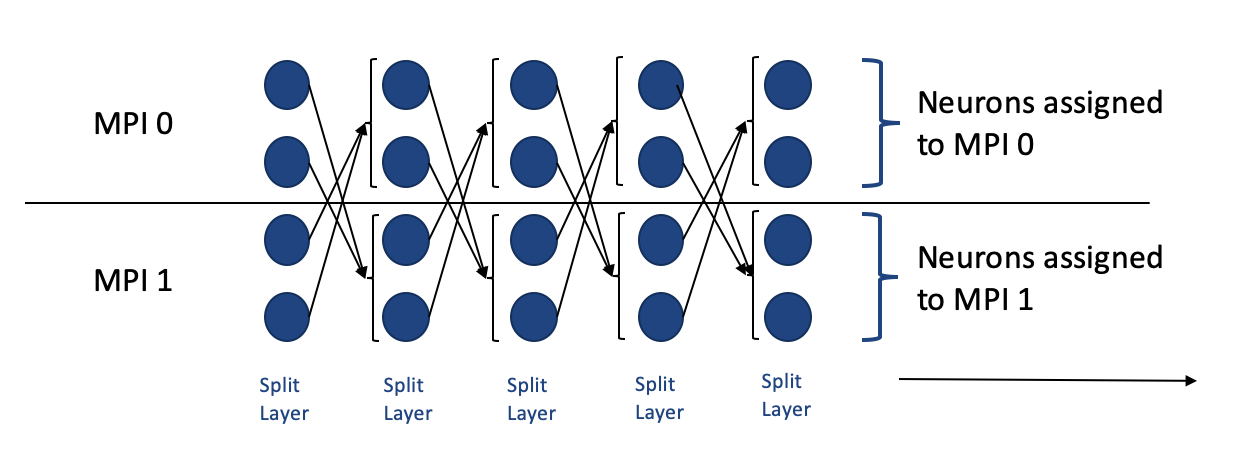
\includegraphics[scale=0.60]{altsplit/figs/baseline.png}}
    \caption{State-of-the-art model parallelism scheme}
    \label{fig:altsplit_baseline}
\end{figure}

We first show the sequential training of a DNN using matrix operations in 
Algorithm~\ref{alg:altsplit_sequential}. We denote $bs$ as the batch size, $L$ 
as the number of layers and $N_l$ as the number of neurons in layer $l$. Matrix 
of layer $l$ is denoted as $\pmb{A}_l[m,n]$ whereas $m$ and $n$ stand for the 
number of rows and columns respectively of the matrix and $(\pmb{A}_l)^T[m,n]$ 
denotes the transpose of the matrix $\pmb{A}_l$ and [m,n] represents the 
dimension of the transposed matrix.  $\nabla \pmb{A}_l[m,n]$ represents the 
gradients of matrix $\pmb{A}_l$. $\phi$ is an element-wise non-linear function 
(tanh, relu etc.). Only the operations on the forward- and backward-propagation 
phases for the hidden layers are shown in detail since they are the regions of 
interest with regard to the subsequent parallel versions of the algorithm.
\begin{algorithm}[H]%algorithm* occupies full page
\caption{Sequential DNN}
\label{alg:altsplit_sequential}
{\fontsize{10}{10}\selectfont
\begin{algorithmic}[1]
    \For {$l = 1 \ldots L$}
    \Comment Forward-propagation \State $\pmb{Y}_l[bs, N_l] = \pmb{O}_{l-1}[bs, N_{l-1}] * (\pmb{W}_{l})^T[N_{l-1}, N_l]$
        \State $\pmb{O}_l[bs, N_l] = \phi(\pmb{Y}[bs, N_l])$
    \EndFor
    \For {$l = L \ldots 1$}
    \Comment Backpropagation 
        \State $\nabla \pmb{W}_l[bs, N_l]  = \nabla \pmb{W}_{l+1}[bs, N_{l+1}] * \pmb{W}_{l+1}[N_{l+1}, N_l]$
        \State $\nabla \pmb{W}_l[bs, N_l] = \nabla \pmb{W}_l[bs, N_l] * (\partial \pmb{O}_l[bs, N_l] / \partial \pmb{Y}_l[bs, N_l]$)
    \EndFor
    \State Update parameters
\end{algorithmic}}
\end{algorithm}

The state-of-the-art model parallelism of a DNN is shown in 
Algorithm~\ref{alg:altsplit_baseline}. Besides the notations we introduced in 
Algorithm~\ref{alg:altsplit_sequential}, we give some additional notations due 
to the introduction of parallelism. $size$ denotes the number of MPI processes, 
$rank$ denotes the ID of the current MPI process and $N_l$ represents the number 
of neurons assigned to each MPI process which is equivalent to 
$N_{l\_total}/size$ (here we assume that $N_{l\_total}/size$ is divisible). This 
algorithm allocates some extra space for holding the information gathered across 
all the MPI threads: 
\begin{itemize}
    \item The weight matrix of each hidden layer $\pmb{W}_l$ should be of dimension 
        $[N_l, N_{l-1}*size]$.
    \item An extra matrix to store the outputs from the preceding hidden layer 
        from all the MPI threads $\pmb{O}_{l-1}[bs, N_{l-1}*size]$.
    \item An extra matrix to store the gradients of the succeeding layer from all 
        the MPI threads $\nabla \pmb{W}_l[bs, N_l*size]$.
\end{itemize}
At the beginning of the forward-propagation phase of each hidden layer an 
\textit{MPI\_Allgather} precedes the computation to gather outputs from all 
local portions from the preceding layer. Subsequently, each MPI thread needs to 
perform a MPI\_Allreduce with the $sum$ operation on $\nabla \pmb{W}_l[bs, 
N_l*size]$ and extract its respective gradients from it during the 
backpropagation phase.

\begin{algorithm}[H]
\caption{State-of-the-art approach to model parallelism of DNN}
\label{alg:altsplit_baseline}
{\fontsize{10}{10}\selectfont
\begin{algorithmic}[1]
    \ForAll {$p \in MPI\_Processes$}
    \Comment Forward-propagation 
        \For {$l = 1 \ldots L$}
            \State MPI\_Allgather on $\pmb{O}_{l-1}[bs, N_{l-1}*size]$ from all local $\pmb{O}_{l-1}[bs, N_{l-1}]$
            \State $\pmb{Y}_l[bs, N_l] = \pmb{O}_{l-1}[bs, N_{l-1}*size] * (\pmb{W}_{l})^T[N_{l-1}*size, N_l]$
            \State $\pmb{O}_l[bs, N_l] = \phi(\pmb{Y}[bs, N_l])$
        \EndFor
    \EndFor
    \ForAll {$p \in MPI\_Processes$}
    \Comment Backpropagation 
        \For {$l = L \ldots 1$}
            \State $\nabla \pmb{W}_l[bs, N_l*size]  = \nabla \pmb{W}_{l+1}[bs, N_{l+1}] * \pmb{W}_{l+1}[N_{l+1}, N_l*size]$
            \State MPI\_Allreduce\_sum on  $\nabla \pmb{W}_l[bs, N_l*size]$
            \State Extract $\nabla \pmb{W}_{l,p}[bs, N_l]$ from $\nabla \pmb{W}_l[bs, N_l*size]$ according to $rank$
            \State $\nabla \pmb{W}_{l,p}[bs, N_l] = \nabla \pmb{W}_{l,p}[bs, N_l] * (\partial \pmb{O}_{l,p}[bs, N_l] / \partial \pmb{Y}_{l,p}[bs, N_l]$)
        \EndFor
    \EndFor
    \ForAll {$p \in MPI\_Processes$}
        \State Update parameters
    \EndFor
\end{algorithmic}}
\end{algorithm}

\subsection{The Altsplit (Alternate Split) Approach}
We propose the \emph{Altsplit} approach which splits or replicates the layers 
alternately. The scheme is illustrated in Figure~\ref{fig:altsplit_scheme} with 
the same 5-hidden-layer DNN as in Figure~\ref{fig:altsplit_baseline}. The first 
hidden layer is split across MPI processes whereas the next layer is replicated 
on the MPI processes with the same initialization values. Subsequent layers are 
constructed with alternating splits and replications. Therefore, we cut the 
amount of communication by half during the entire training compared to the 
\emph{state-of-the-art} approach by triggering communication every other layer while at 
the cost of replicating layers on each MPI process. As a consequence, the floating
point computation is increased by 50\% (twice every other layer).
\begin{figure}[H]
    \centerline{\includegraphics[scale=0.60]{altsplit/figs/altsplit.png}}
    \caption{The \emph{Altsplit} scheme}
    \label{fig:altsplit_scheme}
\end{figure}

Algorithm~\ref{alg:altsplit_altsplit} illustrates the \emph{Altsplit} approach 
to model parallelism. Unlike the state-of-the-art approach, there is no need for extra 
storage in \emph{Altsplit}. If the preceding layer during the 
forward-propagation phase is a split, an MPI\_Allreduce with the \textit{sum} 
operation must be performed on $\pmb{Y}_{l-1}[bs, N_{l}]$. Similarly, the same 
routine must be called upon on $\nabla \pmb{W}_l[bs, N_l]$ while in the 
backpropagation phase if the succeeding layer is a split.

\begin{algorithm}[H]
\caption{\emph{Altsplit} approach to model parallelism of DNN}
\label{alg:altsplit_altsplit}
{\fontsize{10}{10}\selectfont
\begin{algorithmic}[1]
    \ForAll {$p \in MPI\_Processes$}
    \Comment Forward-propagation \For {$l = 1 \ldots L$}
            \State $\pmb{Y}_l[bs, N_l] = \pmb{O}_{l-1}[bs, N_{l-1}] * (\pmb{W}_{l})^T[N_{l-1}, N_l]$
            \If {$l-1 == SPLIT$}
                \State MPI\_Allreduce\_sum on $\pmb{Y}_{l-1}[bs, N_{l}]$ 
            \EndIf
            \State $\pmb{O}_l[bs, N_l] = \phi(\pmb{Y}[bs, N_l])$
        \EndFor
    \EndFor
    \ForAll {$p \in MPI\_Processes$}
    \Comment Backpropagation \For {$l = L \ldots 1$}
            \State $\nabla \pmb{W}_l[bs, N_l]  = \nabla \pmb{W}_{l+1}[bs, 
            N_{l+1}] * \pmb{W}_{l+1}[N_{l+1}, N_l]$
            \If {$l+1 == SPLIT$}
                \State MPI\_Allreduce\_sum on $\nabla \pmb{W}_l[bs, N_l]$
            \EndIf
            \State $\nabla \pmb{W}_{l,p}[bs, N_l] = \nabla \pmb{W}_{l,p}[bs, N_l] * (\partial \pmb{O}_{l,p}[bs, N_l] / \partial \pmb{Y}_{l,p}[bs, N_l]$)
        \EndFor
    \EndFor
    \ForAll {$p \in MPI\_Processes$}
        \State Update parameters
    \EndFor
\end{algorithmic}}
\end{algorithm}

\section{Experimental Setup}
\label{sec:altsplit_setup}
\subsection{Hardware Platforms}
\label{sec:platform}
We conduct our experiments on two clusters featuring the x86 and POWER 
architectures.
The x86 machine is composed of two 8-core Intel Xeon
\textregistered E5-2630 v3 (Haswell) at 2.4 GHz and a 20 MB L3 shared cache 
memory each.  It is also equipped with two Nvidia Tesla K80 accelerators, each 
of which hosts two Tesla GK210 GPUs.
It has 128 GB of main memory, distributed in 8 DIMMs of 16 GB DDR4 @ 2133 MHz.
The 16-core CPU and the four GPUs are connected via a PCIe 3.0 x8 8GT/s.
The operating system is RedHat Linux 6.7.
Overall, the peak performance of the two 8-core sockets plus the four Tesla 
GK210 GPUs is 6.44 TFlop/s.

The POWER machine is composed of two 20-core IBM POWER9 8335-GTG at 3.00 GHz.  
It contains four NVIDIA Volta V100 GPUs.  
Each node has 512 GB of main memory, distributed in 16 DIMMS of 32 GB @ 2666 
MHz.  The GPUs are connected to the CPU devices via a NVIDIA NVLink 2.0 
interconnection~\cite{nvlink}.  The operating system is RedHat Linux 7.4.  The 
peak performance of the two 20-core sockets plus the four V100 GPUs is 28.85 
TFlop/s.

\section{Evalutation}
\label{sec:altsplit_evaluation}
We conduct extensive experiments on various aspects of \emph{Altsplit}. We
demonstrate its scalability in Section~\ref{sec:altsplit_scalability} and
show that it is applicable in different machines by providing results on
two HPC clusters in Section~\ref{sec:altsplit_vers}. In Section~\ref{sec:altsplit_trace}
we visualize the \emph{Altsplit} and the \emph{baseline} approach to get more
insights.

\subsection{Parallelism Scalability}
\label{sec:altsplit_scalability}
We run \emph{Altsplit} and \emph{baseline} side-by-side on the x86 clusters
up to 16 nodes (640 MPI threads). We use a total of 4 configurations of MLP networks: 
\begin{itemize}
   \item 16,000-neuron-per-layer, 3-layer, batch size of 512, denoted as 16000.3.512
   \item 16,000-neuron-per-layer, 3-layer, batch size of 1024, denoted as 16000.3.1024
   \item 16,000-neuron-per-layer, 5-layer, batch size of 512, denoted as 16000.5.512
   \item 16,000-neuron-per-layer, 5-layer, batch size of 1024, denoted as 16000.5.1024
\end{itemize}
We measure the elapse time of runs of 50 batches (51 batches but excluding the result from
the first batch to minimize system noises). We execute them on the dataset from 
Cifar-10~\cite{cifar10}. We use 40 MPI threads per node which are mapped to 40 distinct
physical cores. Hence, the measurements are taken in a stride of 40 MPI threads.

Figure~\ref{fig:altsplit_16k_mn4} shows the results in 4 plots. Each plot 
depicts the performance of \emph{Altsplit} against \emph{baseline} in terms of 
elapse time normalized with regard to \emph{baseline} with varied number of MPI 
threads, from 80 MPI threads (2 nodes) all the way up to 640 MPI threads (16 nodes).

We can see from the top left plot (80 MPI threads) that \emph{Altsplit} goes slower than
\emph{baseline}. Nevertheless, starting from 160 MPI threads (top right) and beyond 
\emph{Altsplit} begins to gain track and consistently outperforms \emph{baseline}. 
More specifically, \emph{Altsplit} runs 18.3\%, 39.32\% and 66.11\% faster than their 
respective \emph{baseline} in average.

\begin{figure}[H]
    \centerline{
        \includegraphics[scale=0.60]{altsplit/figs/mn4/16000_avgs_80.pdf}
        \includegraphics[scale=0.60]{altsplit/figs/mn4/16000_avgs_160.pdf}
    }
    \centerline{
        \includegraphics[scale=0.60]{altsplit/figs/mn4/16000_avgs_320.pdf}
        \includegraphics[scale=0.60]{altsplit/figs/mn4/16000_avgs_640.pdf}
    }
    \caption{Performance improvements of 16k neurons on x86. Top left: 80 MPI 
    processes, Top right: 160 MPI processes, Bottom left: 320 MPI processes, 
    Bottom right: 640 MPI processes}
    \label{fig:altsplit_16k_mn4}
\end{figure}

\subsection{Network Versatility}
\label{sec:altsplit_vers}
We launch a more extensive set of experiment that covers more network
configurations. We use two neurons-per-layer numbers: 16k and 32k, two
layers: 3 and 5 along with two batch sizes: 512 and 1024 on both machines. We
find out that \emph{Altsplit} achieves the greatest performance gain on 640
MPI threads (16 nodes on both machines). Table~\ref{table:altsplit_network}
illustrates the results we obtain from of all the configurations.

We observe that \emph{Altsplit} with 16k neurons-per-layer outperforms
\emph{baseline} over 66.12\% and 55.47\% on x86 and POWER9 respectively
whereas with 32k neurons-per-layer the figures are 41.10\% and 32.64\%
respectively. A low neuron-per-layer count attributes to a better performance
with an average gain in average of 25.02\% and 24.51\% respectively on x86
and POWER9. Since we are effectively trading communication with additional
computation with the \emph{Altsplit} approach. In general \emph{Altsplit} also
performs better under smaller batch sizes. This indicates that there is a sweet 
spot where the benefit of reducing the communication is maximized.

\begin{table}[H]
\caption{Performance improvements over the \emph{baseline} on 640 MPI threads}
    \centering
    \begin{tabular}{|P{2.5cm}|P{2.5cm}|P{2.5cm}|P{2.5cm}|P{2.5cm}|}
    \hline
    \multicolumn{3}{|c}{Parameters} & \multicolumn{2}{|c|}{Machine} \\ \hline
    Neurons & Layers & BS & \textbf{x86}  & \textbf{POWER9}  \\ \hline
    \multirow{4}{*}{16k} & \multirow{2}{*}{3} & 512 & 68.12\%& 58.65\%
        \\ \cline{3-5}
     & & 1024 & 61.47\% & 56.12\%
        \\ \cline{2-5}
     & \multirow{2}{*}{5} & 512 & 68.21\%& 58.43\%
        \\ \cline{3-5}
     & & 1024 & 66.68\%& 55.47\%
        \\ \hline 
    \multicolumn{3}{|c|}{Average} & 66.12\% & 57.16\% \\ \hline
     \multirow{4}{*}{32k} & \multirow{2}{*}{3} & 512 & 45.28\% & 32.75\%
        \\ \cline{3-5}
     & & 1024 & 37.69\% & 31.58\%
        \\ \cline{2-5}
     & \multirow{2}{*}{5} & 512 & 43.87\% & 34.37\%
        \\ \cline{3-5}
     & & 1024 & 37.58\%& 31.91\%
        \\ \hline 
    \multicolumn{3}{|c|}{Average} & 41.10\% & 32.65\% \\ \hline
\end{tabular}
\label{table:altsplit_network}
\end{table}


\subsection{Traces}
\label{sec:altsplit_trace}
We run both the \emph{Altsplit} and \emph{baseline} on the x86 cluster with
80 MPI threads and generate running traces. Figure~\ref{fig:altsplit_traces}
illustrates a run with 10 batches (9 are actually shown to exclude the system
noises introduced by the first batch). The x-axis represents the elapse time
whereas each row from the y-axis is the chronological activity from one of
the 80 MPI threads. MPI calls are displayed as the short burst of colored
lines in the traces and the blank areas represents computation or other
system activities. Their length are proportional to the total elapse time.
Two types of MPI all-to-all communication involved in the \emph{baseline}
implementation, namely, MPI\_Allreduce and MPI\_Allgather which corresponds
with the trace on the top. Those marked with red are calls from
MPI\_Allgather while the pink ones are calls from MPI\_Allreduce. The
duration of the trace of the \emph{Altsplit} is the same as in the
\emph{baseline}. One batch in the trace of the \emph{baseline} is marked with
two consecutive MPI\_Allgather (red) calls followed with two MPI\_Allreduce
(pink) ones. On the other hand, in the trace of \emph{Altsplit} one batch is
marked with two MPI\_Allreduce calls with a blank area sparsely dotted with small
bursts of MPI calls. The dark blue activities displayed at the end of both
traces are MPI\_Finalize calls to mark the end of the MPI execution.

We can see that despite the similar duration of MPI\_Allreduce calls on both
approaches and the fact that it takes a longer time for the \emph{Altsplit} to 
commence the subsequent batch, the additional MPI\_Allgather incur a significant 
slow down compared to the blank area in-between the successive MPI\_Allreduce 
calls from the \emph{Altsplit} approach.

\begin{figure}[H]
    \centerline{\includegraphics[scale=0.30]{altsplit/figs/baseline_trace.png}}
    \centerline{\includegraphics[scale=0.30]{altsplit/figs/altsplit_trace.png}}
    \caption{Traces on 80 MPI processes 9 batches. Top: \emph{baseline} approach Bottom: \emph{altsplit} approach}
    \label{fig:altsplit_traces}
\end{figure}

\section{Conclusions}
\label{sec:altsplit_conclusion}
This chapter presents the \emph{Altsplit} approach that intends to provide a
model parallelism of the DNN with less communication. It achieves this by
distributing the neurons and replicating them across all the computational
units alternately in-between successive layers so that all-to-all
communication only occurs every other layers instead of in a lock-step
fashion in an \emph{na\"{i}ve} approach. Our experiments are conducted taking
multiple hyper-parameters into consideration: the number of neurons per
layer, the number of layers and batch sizes. We conduct the experiments on
two high-end multicore multinode clusters with distinct CPU architecture.

We find that the \emph{Altsplit} approach achieves significant speedups over
our baseline \emph{na\"{i}ve} approach regardless the underlying cluster.
Furthermore, we show that the speedup is retained among various
hyper-parameters and we visualize the speedup by generating traces on both
approach and shows that the trade-off between additional floating-point 
computations and reduced communication pays off.

\chapter{Conclusions}
\label{chap:conclusions}
This thesis intends to alleviate the bottlenecks brought about by all-to-all 
communication in the modern HPC systems due to the constant scaling-up of the 
system size, problem size and the appearances of emerging fields.
This proves to be a daunting task because there is not an one-size-fits-all 
approach to it. Each field possesses its own requirements and patterns on 
communication. Furthermore, the trade-offs applicable differ from field to 
field.

This thesis utilizes three trade-off techniques in concrete for the communication 
reduction purpose.
\begin{itemize}
    \item Exploiting the resilience towards accumulation of rounding errors and 
        loss of precision of the problem at hand to reduce communication.
    \item Trading with a decreased computational precision with a marginal 
        deterioration of the accuracy of the problem for reduced amount of 
        communication. 
    \item Trading at the cost of additional computation with reduce amount of 
        communication.
\end{itemize}

The thesis first takes on reducing communication in one of the Krylov iterative 
methods, CG. Compare to the various available direct methods the CG method 
displays greater tolerance towards the accumulation of rounding errors. We thus 
fuse a certain amount of iterations together which means some efforts to bring 
down the accumulated error such as the residual replacement strategy has to be 
deferred to the end of the fused phase. Nevertheless, we show that further 
incorporating a task-based parallelism approach, significant speedup can be 
achieved without much hampering to the convergence of the algorithm.

On tackling the problem of accelerating the DNN training with multiple GPUs, we 
exploited the fact that DNNs are intrinsically tolerant to a lowered precision 
of both its parameters. Guided by the L2-norm of the weights of each layer, we 
start by transferring compressed weights with low precision and dynamically 
increment the precision in a per-layer granularity if needed.
Our experiments confirms that this approach greatly reduces the amount of data
needed to be transferred from the CPU host to GPUs prior to the beginning of 
each batch and consequently outperforms the training with full 32-bit floating 
point weights in terms of the training time.

In order to remove some amount of communication from applying model parallelism 
to DNNs, we try to replicate every other layers rather than splitting each and 
every layer so that communication only occurs once every two layers. Despite the 
higher count of computation inevitably introduced by the approach, our 
experiments indicate that it is a trade-off well justified. It outperforms our 
baseline approach by a large margin on two high-end clusters with completely 
distinct CPU architectures. 

\section{Further Down The Road}
With the first exascale clusters on the horizon, the pursuit of more accurate 
models in computational sciences and the awe-inspiring speed deep learning and 
data science are taking over multiple industries, the potential benefit for a 
communication-reduction solution to a particular problem will not diminish any 
time soon. The techniques this thesis explores all come off as trade-offs of 
various sorts since communication is closely entangled with other aspects of the 
algorithm: computation, space, precision etc. A deeper understanding into their 
synergy on an per-algorithm basis is of great importance. Furthermore, we need 
some level of generalization to derive techniques that are applicable to 
multiple fields.  

%As of deep neural network, extensive research has been conducted on reduce the 

\begin{appendices}
\chapter{Publications}
\section{Publications Related With The Thesis}
\begin{itemize}
	\item \bibentry{ifcg}
	\item Sicong Zhuang, Cristiano Malossi and Marc Casas. Reducing Data Motion 
        to Accelerate the Training of Deep Neural Networks (submitted to IPDPS'20)
	\item Sicong Zhuang, Panagiotis Hadjidoukas, Cristiano Malossi and Marc 
        Casas. Altsplit: Communication Reduction In DNN Model Parallelism 
        (future submission)
\end{itemize}

\section{Other Publications}
\begin{itemize}
    \item \bibentry{ilia}
\end{itemize}

\chapter{Pragmas}
\section{Description}
The following are the list of the \textit{pragma} annotations of the routines 
used in the various CG implementations of Chapter~\ref{chap:ifcg}. The 
source code is open source and can be downloaded from
\href{git@github.com:zhuangsc/IFCG.git}{Github}. The annotations follow the 
syntax and semantics of the OmpSs programming model. The exact definitions 
of those annotations can be found at the
\href{https://pm.bsc.es/ftp/ompss/doc/spec/}{OmpSs official page}.

\section{Annotations}
\begin{lstlisting}
#pragma omp task in(X[initx:initx+bm-1], Y[inity:inity+bm-1]) concurrent(result[0:bn-1]) no_copy_deps priority(p) label(ddot) 
void __t_dot(int p, int bm, int bn, int m, int n, double *X, double *Y, int initx, int inity, double *result); 

#pragma omp task in(X1[0:bm-1], X2[0:bm-1], Anum[0:bn-1], Aden[0:bn-1], Y1[0:bm-1], Y2[0:bm-1]) out(Z1[0:bm-1], Z2[0:bm-1]) no_copy_deps priority(1) label(dcpaxpy_comb)
void __t_cpaxpy_comb(int bm, int bn, int m, int n, double alpha, double *Anum, double *Aden, double *X1, double *X2, double *Y1, double *Y2, double *Z1, double *Z2);

#pragma omp task in(X[0:bm-1], Y[0:bm-1], SAnum[0:bn-1], SAden[0:bn-1]) out(Z[0:bm-1]) no_copy_deps priority(p) label(extm_axpy)
void __t_extm_axpy(int bm, int bn, int m, int n, double *SAnum, double *SAden, double *X, double *Y, double *Z, int p);

#pragma omp task in(X[initx:initx+bm-1], Y[inity:inity+bm-1], A[inita:inita+bm-1], B[initb:initb+bm-1]) concurrent([bn]result, [bn]result2) no_copy_deps priority(p) label(cg_dot2)
void _cg_dot2(int p, int bm, int bn, int m, int n, double *X, double *Y, int initx, int inity, double *result, double *A, double *B, int inita, int initb, double *result2);

/* Computation of the coefficients */
#pragma omp task in(gamma[i], delta) out(beta[i], alpha[i]) label(centinel) 
{
    if ( k > 0 ) {
        beta[i] = gamma[i]/gamma[iprev];
        alpha[i] = gamma[i] / (delta - beta[i] * gamma[i] / alpha[iprev]);
    } else {
        beta[i] = (double) 0;
        alpha[i] = gamma[i]/delta;
    }
    gamma[iprev] = delta = 0;
}  
\end{lstlisting}
\end{appendices}






% ********************************** Back Matter *******************************
% Backmatter should be commented out, if you are using appendices after References
%\backmatter

% ********************************** Bibliography ******************************
\begin{spacing}{0.9}

% To use the conventional natbib style referencing
% Bibliography style previews: http://nodonn.tipido.net/bibstyle.php
% Reference styles: http://sites.stat.psu.edu/~surajit/present/bib.htm


%\bibliographystyle{apalike} % Use for unsorted references  
\bibliographystyle{unsrt} % Use for unsorted references  
%\bibliographystyle{plainnat} % use this to have URLs listed in References
\cleardoublepage
\bibliography{references/biblio} % Path to your References.bib file


% If you would like to use BibLaTeX for your references, pass `custombib' as
% an option in the document class. The location of 'reference.bib' should be
% specified in the preamble.tex file in the custombib section.
% Comment out the lines related to natbib above and uncomment the following line.

%\printbibliography[heading=bibintoc, title={References}]


\end{spacing}

% ********************************** Appendices ********************************

%\begin{appendices} % Using appendices environment for more functunality

%\include{Appendix1/appendix1}
%\include{Appendix2/appendix2}

%\end{appendices}

% *************************************** Index ********************************
\printthesisindex % If index is present

\listoffigures
\listoftables
\printglossary[type=\acronymtype, style=long, nonumberlist, title=List of Abbreviations]

\end{document}

